\documentclass{article}

% if you need to pass options to natbib, use, e.g.:
%     \PassOptionsToPackage{numbers, compress}{natbib}
% before loading neurips_2019

% ready for submission
\usepackage{neurips_2019}

% to compile a preprint version, e.g., for submission to arXiv, add add the
% [preprint] option:
%     \usepackage[preprint]{neurips_2019}

% to compile a camera-ready version, add the [final] option, e.g.:
     % \usepackage[final]{neurips_2019}

% to avoid loading the natbib package, add option nonatbib:
%     \usepackage[nonatbib]{neurips_2019}

\usepackage[utf8]{inputenc} % allow utf-8 input
\usepackage[T1]{fontenc}    % use 8-bit T1 fonts
\usepackage{hyperref}       % hyperlinks
\usepackage{url}            % simple URL typesetting
\usepackage{booktabs}       % professional-quality tables
\usepackage{amsfonts}       % blackboard math symbols
\usepackage{nicefrac}       % compact symbols for 1/2, etc.
\usepackage{microtype}      % microtypography
\usepackage{amsthm}     % for theorems
\usepackage{algorithm,algorithmic}
\usepackage{mathtools}
\usepackage{amsmath}
\allowdisplaybreaks
\usepackage{amssymb}
\DeclarePairedDelimiter{\norm}{\lVert}{\rVert}
\usepackage{balance}
\usepackage{comment}
\newcommand{\eq}[1]{{Eq~(#1)}}
\newcommand{\figref}[1]{Figure~\ref{#1}}
\newtheorem{theorem}{Theorem}
\newtheorem{thm}{Theorem}
\newtheorem{lemma}[theorem]{Lemma}
\newtheorem{remark}{Remark}
\newcommand{\lkxcom}[1]{{\color{red}{#1}}}

\newcommand{\ov}[1]{{\overline{\mathbf{#1}}}}
%% common packages
\usepackage{amsbsy}
\usepackage{amsmath}
\usepackage{graphicx}
\usepackage{subfigure}
\usepackage{color}
\usepackage{booktabs}

%% to allow citation as footnote
\usepackage{natbib}
% and to reduce footnote font size
\usepackage{etoolbox}
\makeatletter
\patchcmd{\@makefntext}{\insertfootnotetext{#1}}{\insertfootnotetext{\scriptsize#1}}{}{}
\makeatother


%% macros for commenting
\usepackage[normalem]{ulem} % to use \sout
\newcommand{\remove}[1]{{\color{Gray}\sout{#1}}}
\newcommand{\revise}[1]{{\color{blue}#1}}
\newcommand{\commwy}[1]{{\color{red}(wy: #1)}} % Wotao Yin

%% template for beamer

%\mode<presentation>
%{
%  % page number
%  %\setbeamertemplate{footline}{\insertframenumber/\inserttotalframenumber}
%  \setbeamertemplate{footline}[frame number]
%
%  % background and theme
%  \setbeamertemplate{background canvas}[vertical shading][bottom=white!10,top=white!10]
%  \usetheme{default}
%
%  % section in table of contents has numbers
%  \setbeamertemplate{sections/subsections in toc}[sections numbered]
%
%  % no navigation bottoms
%  \setbeamertemplate{navigation symbols}{}
%
%  % itemize, black bullet, %150 spacing between items using "witemize"
%  \setbeamertemplate{itemize items}[circle]
%  \setbeamercolor{itemize item}{fg=black}
%  \setbeamercolor{enumerate item}{fg=black}
%  \setbeamercolor{itemize subitem}{fg=black}
%  \setbeamercolor{enumerate subitem}{fg=black}
%  \newenvironment{witemize}{\itemize\addtolength{\itemsep}{0.0\baselineskip}}{\enditemize}
%
%  % block, black over gray with no shadow
%  \setbeamertemplate{blocks}[rounded][shadow=false]
%  \setbeamercolor{block title}{fg=black,bg=gray!40}
%  \setbeamercolor{block body}{fg=black,bg=gray!10}
%
%  % frametitle, bold, black, centered
%  \setbeamertemplate{frametitle}[default][center]
%  \setbeamercolor{frametitle}{fg=black}
%  \setbeamerfont{frametitle}{shape=\bfseries}
%
%  % line spacing
%  \linespread{1.2}
%
%  \setlength{\parskip}{\smallskipamount}
%}

%% macros for letters

\newcommand{\va}{{\mathbf{a}}}
\newcommand{\vb}{{\mathbf{b}}}
\newcommand{\vc}{{\mathbf{c}}}
\newcommand{\vd}{{\mathbf{d}}}
\newcommand{\ve}{{\mathbf{e}}}
\newcommand{\vf}{{\mathbf{f}}}
\newcommand{\vg}{{\mathbf{g}}}
\newcommand{\vh}{{\mathbf{h}}}
\newcommand{\vi}{{\mathbf{i}}}
\newcommand{\vj}{{\mathbf{j}}}
\newcommand{\vk}{{\mathbf{k}}}
\newcommand{\vl}{{\mathbf{l}}}
\newcommand{\vm}{{\mathbf{m}}}
\newcommand{\vn}{{\mathbf{n}}}
\newcommand{\vo}{{\mathbf{o}}}
\newcommand{\vp}{{\mathbf{p}}}
\newcommand{\vq}{{\mathbf{q}}}
\newcommand{\vr}{{\mathbf{r}}}
\newcommand{\vs}{{\mathbf{s}}}
\newcommand{\vt}{{\mathbf{t}}}
\newcommand{\vu}{{\mathbf{u}}}
\newcommand{\vv}{{\mathbf{v}}}
\newcommand{\vw}{{\mathbf{w}}}
\newcommand{\vx}{{\mathbf{x}}}
\newcommand{\vy}{{\mathbf{y}}}
\newcommand{\vz}{{\mathbf{z}}}

\newcommand{\vA}{{\mathbf{A}}}
\newcommand{\vB}{{\mathbf{B}}}
\newcommand{\vC}{{\mathbf{C}}}
\newcommand{\vD}{{\mathbf{D}}}
\newcommand{\vE}{{\mathbf{E}}}
\newcommand{\vF}{{\mathbf{F}}}
\newcommand{\vG}{{\mathbf{G}}}
\newcommand{\vH}{{\mathbf{H}}}
\newcommand{\vI}{{\mathbf{I}}}
\newcommand{\vJ}{{\mathbf{J}}}
\newcommand{\vK}{{\mathbf{K}}}
\newcommand{\vL}{{\mathbf{L}}}
\newcommand{\vM}{{\mathbf{M}}}
\newcommand{\vN}{{\mathbf{N}}}
\newcommand{\vO}{{\mathbf{O}}}
\newcommand{\vP}{{\mathbf{P}}}
\newcommand{\vQ}{{\mathbf{Q}}}
\newcommand{\vR}{{\mathbf{R}}}
\newcommand{\vS}{{\mathbf{S}}}
\newcommand{\vT}{{\mathbf{T}}}
\newcommand{\vU}{{\mathbf{U}}}
\newcommand{\vV}{{\mathbf{V}}}
\newcommand{\vW}{{\mathbf{W}}}
\newcommand{\vX}{{\mathbf{X}}}
\newcommand{\vY}{{\mathbf{Y}}}
\newcommand{\vZ}{{\mathbf{Z}}}

\newcommand{\cA}{{\mathcal{A}}}
\newcommand{\cB}{{\mathcal{B}}}
\newcommand{\cC}{{\mathcal{C}}}
\newcommand{\cD}{{\mathcal{D}}}
\newcommand{\cE}{{\mathcal{E}}}
\newcommand{\cF}{{\mathcal{F}}}
\newcommand{\cG}{{\mathcal{G}}}
\newcommand{\cH}{{\mathcal{H}}}
\newcommand{\cI}{{\mathcal{I}}}
\newcommand{\cJ}{{\mathcal{J}}}
\newcommand{\cK}{{\mathcal{K}}}
\newcommand{\cL}{{\mathcal{L}}}
\newcommand{\cM}{{\mathcal{M}}}
\newcommand{\cN}{{\mathcal{N}}}
\newcommand{\cO}{{\mathcal{O}}}
\newcommand{\cP}{{\mathcal{P}}}
\newcommand{\cQ}{{\mathcal{Q}}}
\newcommand{\cR}{{\mathcal{R}}}
\newcommand{\cS}{{\mathcal{S}}}
\newcommand{\cT}{{\mathcal{T}}}
\newcommand{\cU}{{\mathcal{U}}}
\newcommand{\cV}{{\mathcal{V}}}
\newcommand{\cW}{{\mathcal{W}}}
\newcommand{\cX}{{\mathcal{X}}}
\newcommand{\cY}{{\mathcal{Y}}}
\newcommand{\cZ}{{\mathcal{Z}}}

\newcommand{\ri}{{\mathrm{i}}}
\newcommand{\rr}{{\mathrm{r}}}


%% macros for math notions and operators

\newcommand{\RR}{\mathbb{R}}
\newcommand{\EE}{\mathbb{E}}
\newcommand{\CC}{\mathbb{C}}
\newcommand{\ZZ}{\mathbb{Z}}
\renewcommand{\SS}{{\mathbb{S}}}
\newcommand{\SSp}{\mathbb{S}_{+}}
\newcommand{\SSpp}{\mathbb{S}_{++}}
\newcommand{\sign}{\mathrm{sign}}
\newcommand{\Sign}{\mathrm{Sign}}
\newcommand{\vzero}{\mathbf{0}}
\newcommand{\vone}{{\mathbf{1}}}
\newcommand{\Null}{{\mathrm{Null}}}
\newcommand{\dist}{{\mathrm{dist}}}
\newcommand{\Co}{{\mathbf{Co}}}

\newcommand{\op}{{\mathrm{op}}} % subscript for operator norm
\newcommand{\opt}{{\mathrm{opt}}} % subscript for optimal solution
\newcommand{\supp}{{\mathrm{supp}}} % support
\newcommand{\Prob}{{\mathrm{Prob}}} % probability
\newcommand{\Diag}{{\mathrm{Diag}}} % vector -> diagonal matrix
\newcommand{\diag}{{\mathrm{diag}}} % matrix diagonal -> vector
\newcommand{\dom}{{\mathrm{dom}}} % domain
\newcommand{\grad}{{\nabla}}    % gradient
\newcommand{\tr}{{\mathrm{tr}}} % trace
\newcommand{\TV}{{\mathrm{TV}}} % total variation
\newcommand{\Proj}{{\mathrm{Proj}}}
\DeclareMathOperator{\shrink}{shrink} % shrinkage
\DeclareMathOperator*{\argmin}{arg\,min}
\DeclareMathOperator*{\argmax}{arg\,max}
\DeclareMathOperator*{\mini}{minimize}
\DeclareMathOperator*{\maxi}{maximize}
\DeclareMathOperator*{\Min}{minimize}
\DeclareMathOperator*{\Max}{maximize}
\newcommand{\prox}{{\mathbf{prox}}}
\newcommand{\st}{{\quad\text{s.t.}~}}

%% macros for environments math equations

\newcommand{\MyFigure}[1]{../fig/#1}

\newcommand{\bc}{\begin{center}}
\newcommand{\ec}{\end{center}}

\newcommand{\bdm}{\begin{displaymath}}
\newcommand{\edm}{\end{displaymath}}

\newcommand{\beq}{\begin{equation}}
\newcommand{\eeq}{\end{equation}}

\newcommand{\bfl}{\begin{flushleft}}
\newcommand{\efl}{\end{flushleft}}

\newcommand{\bt}{\begin{tabbing}}
\newcommand{\et}{\end{tabbing}}

\newcommand{\beqn}{\begin{eqnarray}}
\newcommand{\eeqn}{\end{eqnarray}}

\newcommand{\beqs}{\begin{align*}} % no equation numbers
\newcommand{\eeqs}{\end{align*}}  % no equation numbers

%% macros for theorem-like environments

% \newtheorem{theorem}{Theorem}
% \newtheorem{condition}{Condition}
\newtheorem{assumption}{Assumption}
\newtheorem{definition}{Definition}
% \newtheorem{corollary}{Corollary}
% \newtheorem{remark}{Remark}
% \newtheorem{lemma}{Lemma}
% \newtheorem{proof}{Proof}
% \newtheorem{proof*}{Proof}
% \newtheorem{proposition}{Proposition}
%\newtheorem{example}{Example}

% \newtheorem{example}[remark]{Example}



\newtheorem*{assumption*}{Assumption}

\title{Unified Convergence Analysis of FedAve on Non-IID Data}

\author{}

\begin{document}

\maketitle

% \tableofcontents
% \begin{abstract}
% \end{abstract}


% converge proof
% Introduction.

% accelerated 
% convex strongly 
% smooth non-smooth. 
% !TEX ROOT=./main.tex


\section{Problem Setting}

\begin{align}
	\min _{\mathbf{w}}\left\{F(\mathbf{w}) \triangleq \sum_{k=1}^{N} p_{k} F_{k}(\mathbf{w})\right\}
	\label{eq:problem}
\end{align}
where $N$ is the number of devices, and $p_k$ is the weight of the k-th device
such that $p_k \geq 0$ and $\sum_{k=1}^N p_k = 1$. Suppose the k-th device
holds the nk training data: $x_{k,1}, x_{k,2}, \dots, x_{k,n_k}$ . The local
$k \in S_t^K$ objective $F_k(\cdot)$ is defined by

\begin{align}
F_{k}(\mathbf{w}) \triangleq \frac{1}{n_{k}} \sum_{j=1}^{n_{k}} \ell\left(\mathbf{w} ; x_{k, j}\right)	
\label{eq:localloss}
\end{align}

% The summary of all assumptions:

% \begin{assumption}
% $F_{1}, \cdots, F_{N}$ are all $L$-smooth: for all  $\mathbf{v}$  and $\mathbf{w}$, $F_{k}(\mathbf{v}) \leq F_{k}(\mathbf{w})+(\mathbf{v}- \\ \mathbf{w})^{T} \nabla F_{k}(\mathbf{w})+\frac{L}{2}\|\mathbf{v}-\mathbf{w}\|_{2}^{2}$.
% \end{assumption}

% \begin{assumption}
% $F_1,\dots, F_N$ are all convex: for all $\vv$ and $\vw$, 
% $F_k(\vv) \geq F_k(\vw)+(\vv -\vw)^T \grad F_k(\vw)$. \label{ass:cvx}
% \end{assumption}
% \begin{assumption}
% $	F_{1}, \cdots, F_{N} \text { are all } \mu \text { -strongly convex: for all v and } \mathbf{w}, F_{k}(\mathbf{v}) \geq F_{k}(\mathbf{w})+(\mathbf{v}- \\ \mathbf{w})^{T} \nabla F_{k}(\mathbf{w})+\frac{\mu}{2}\|\mathbf{v}-\mathbf{w}\|_{2}^{2}$
% \end{assumption}

% \begin{assumption}
% Let $\xi_{t}^{k}$ be sampled from the k-th device's local data uniformly at random. The variance of stochastic gradients in each device is bounded:
% $\mathbb{E}\left\|\nabla F_{k}\left(\mathbf{w}_{t}^{k}, \xi_{t}^{k}\right)-\nabla F_{k}\left(\mathbf{w}_{t}^{k}\right)\right\|^{2} \leq \sigma_{k}^{2}$, for $k = 1,..., N$.
% \end{assumption}

% \begin{assumption}
% The expected squared norm of stochastic gradients is uniformly bounded. i.e.,
% $\mathbb{E}\left\|\nabla F_{k}\left(\mathbf{w}_{t}^{k}, \xi_{t}^{k}\right)\right\|^{2} \leq G^{2}$, for all $k = 1,..., N$ and $t=0, \dots, T-1$.
% \end{assumption}

\section{Notations}


Let $\vw_t^k$ be the model parameter maintained in the k-th device at the t-th step. $\cI_E$ is a set of global synchronization steps, i.e., $\cI_E = \{n E|n = 1, 2, 3,\dots \}$. If $t+1 \in \cI_E$, which means we communicate the server with (all) clients at time step $t+1$. $\vv^k_{t+1}$ is the immediate result of one step SGD update from $\vw^k_{t}$.
$\xi_{t}^{k}$ denotes the data sampled from k-th device’s local data uniformly at random.
Follow the common practice, we define two virtual sequences $\overline{\mathbf{v}}_{t}$ and $\overline{\mathbf{w}}_{t}$. For full device participation and $t \notin \cI_E$,
$\ov{v}_t = \ov{w}_t =\sum_{k=1}^{N} p_{k} \mathbf{v}_{t}^{k}$. In partial participation, $t \in \cI_E$, $\ov{w}_t \neq \ov{v}_t$ since $\ov{v}_t=\sum_{k=1}^{N} p_{k} \mathbf{v}_{t}^{k}$ while $\sum_{k\in \cS_t}\mathbf{w}_{t}^{k}$. However, we can
set unbiased sampling strategy such that $ \EE_{\cS_t} \ov{w}_t = \ov{v}_t$.
$\overline{\mathbf{v}}_{t+1}$ is one-step SGD from $\overline{\mathbf{w}}_{t}$. 
\begin{align}
\overline{\mathbf{v}}_{t+1}=\overline{\mathbf{w}}_{t}-\eta_{t} \mathbf{g}_{t}	\label{eq:vbar}
\end{align}
% $t+1 \in \cI_E$, we can fetch $\overline{\vw}_{t+1}$, we can communicate $\overline{\vw}_{t+1}$ to all devices.
where $\vg_{t} = \sum_{k=1}^{N} p_{k} \vg_{t,k} $ is one-step stochastic gradient, averaged over all devices. 
\begin{align}
\vg_{t,k} \left\{\begin{array}{ll} 
 = \nabla F_{k}\left(\mathbf{w}_{t}^{k},\xi_{t}^{k} \right)  &  \text{smooth}\\
 \in \partial F_{k}\left(w_{t}^{k}, \xi_{t}^{k}\right)  & \text{non-smooth}
 \end{array}\right.
\end{align}
Similarly, we denote the expected one-step gradient $\ov{g}_{t}= \EE_{\xi_t}[\vg_t] = \sum_{k=1}^{N} p_{k} \EE_{\xi_{t}^{k}} \vg_{t,k}$, where
\begin{align}
\EE_{\xi_{t}^{k}} \vg_{t,k}  \left\{\begin{array}{ll} 
 = \nabla F_{k}\left(\mathbf{w}_{t}^{k}\right)  &  \text{smooth}\\
 \in \partial F_{k}\left(w_{t}^{k}\right)  & \text{non-smooth}
 \end{array}\right.
\end{align}
and we use $\xi_t = \{\xi_t^k\}_{k=1}^N$ denotes samples at all devices at time step $t$. 

The updates of FedAve with partial device activation is given by: 
\begin{align} 
\mathbf{v}_{t+1}^{k} &=\mathbf{w}_{t}^{k}-\eta_{t} \nabla F_{k}\left(\mathbf{w}_{t}^{k}, \xi_{t}^{k}\right) \\ \mathbf{w}_{t+1}^{k} &=\left\{\begin{array}{ll}\mathbf{v}_{t+1}^{k} & \text { if } t+1 \notin \mathcal{I}_{E}, \\ 
\sum_{k \in \cS_{t+1}} \mathbf{v}_{t+1}^{k} & \text { if } t+1 \in \mathcal{I}_{E}\end{array}\right.
\end{align}

In~\cite{li2019convergence}, two types of unbiased sampling strategies are considered in Lemma 5. 
The sampling scheme I establishes $\cS_{t+1}$ by i.i.d. sampling the devices with replacement,
in this case the upper bound of expected square norm of $\ov{w}_{t+1} - \ov{v}_{t+1}$ is given by:
\begin{align}
\EE_{\cS_{t+1}}\left\|\ov{w}_{t+1} - \ov{v}_{t+1}\right\|^2	\leq \frac{4}{K} \eta_t^2 E^2G^2
\end{align}
The sampling scheme II establishes $\cS_{t+1}$ by uniformly sampling all devices without
replacement, in which we have the 
\begin{align}
\EE_{\cS_{t+1}}\left\|\ov{w}_{t+1} - \ov{v}_{t+1}\right\|^2	\leq \frac{4(N - K)}{K(N-1)} \eta_t^2 E^2G^2
\end{align}
We denote this upper bound as follows for concise presentation. 
\begin{align}
	\EE_{\cS_{t+1}}\left\|\ov{w}_{t+1} - \ov{v}_{t+1}\right\|^2 \leq  \eta_t^2 C
	\label{eq:partialsample}
\end{align}


\lkxcom{Questions and next steps}
\begin{itemize}
	\item Consider heterogeneity of data: with strongly convex and smooth, we can use optimality gap. with non-smooth, we can use weighted gradient diversity. 
	\item Nonconvex imply strongly convex: KDD~\cite{zhuo2019federated} has constant learning rate, in our case, we have a diminishing learning rate. 
	\item Quantify biased sampling scheme?
	\item Constant learning rate in other non-strongly convex case. 
\end{itemize}



% !TEX ROOT=./main.tex



\section{Convergence Results}
This section summarizes the current results and assumptions.
\begin{table}[h!]
\centering
\small
	\begin{tabular}{|c|c|c|c|c|}\hline
		paper         &  Cvx Non-smth & Cvx L-smth & Strongly Cvx Non-smth& Strongly Cvx L-smth \\ \hline
	Accelerated	SGD   &   $\cO(\frac{1}{\sqrt{T}})$     & $\cO(\frac{1}{\sqrt{T}})$   &    $\cO(\frac{1}{T})$   &  $\cO(\frac{1}{T})$    \\\hline
	SGD    &    $\cO(\frac{1}{\sqrt{T}})$  &   $\cO(\frac{1}{\sqrt{NT}})$  &  $\cO(\frac{1}{T})$  & $\cO(\frac{1}{T})$\cite{li2019convergence,haddadpour2019convergence}, $\cO(\frac{1}{NT})$ ours    \\\hline
	\end{tabular}
	\caption{Summarize of related work on federated learning, heterogeneous data.}
\end{table}

Acceleration of MaSS for linear regression, partial participation
also $O((1+\frac{4}{K}\cdot(\frac{t}{E}-1))\exp(-\frac{t}{\sqrt{\kappa_{m}\tilde{\kappa}_{m}}}))$
over $O((1+\frac{4}{K}\cdot(\frac{t}{E}-1))\exp(-\frac{t}{\kappa_{m}}))$. 

Linear speedup of SGD and Nesterov SGD for strongly convex and smooth
objectives: full participation $O(\frac{\nu_{max}^{2}\sigma^{2}}{NT}+\frac{E^{2}LG^{2}}{T^{2}})$
with $\nu_{max}=N\cdot\max_{k}p_{k}$; partial participation $O(\frac{\nu_{max}^{2}\sigma^{2}+4E^{2}G^{2}L}{KT})$.
In particular, this implies full participation allows $E=O(\sqrt{\frac{T}{N}})$
to achieve $O(1/NT)$, whereas partial participation only allows $E=O(1)$
to achieve $O(1/KT)$. 

Other accelerations likely not possible. 


\begin{assumption}[Bounded local variance]
Let $\xi_{t}^{k}$ be sampled from the $k$ -th device's local data uniformly at random. The variance of stochastic gradients in each device is bounded: $\mathbb{E}\left\|\nabla F_{k}\left(\mathbf{w}_{t}^{k}, \xi_{t}^{k}\right)-\nabla F_{k}\left(\mathbf{w}_{t}^{k}\right)\right\|^{2} \leq \sigma_{k}^{2}$,
for $k=1, \cdots, N$.	
\end{assumption}



% \begin{assumption}
% The expected squared norm of stochastic subgradients is uniformly bounded. i.e.,
% $\mathbb{E}\|\vg_{t,k}\|^2  \leq G_k^{2}$, for all $k = 1,..., N$ and $t=0, \dots, T-1$.  This also implies $\left\| \mathbb{E}\vg_{t,k}\right\|^2  \leq \mathbb{E}\|\vg_{t,k}\|^2 \leq G_k^2$. Denote $G^2 = \sum_{k=1}^N p_k G_k^2$
% \label{ass:subgrad2}
% \end{assumption}


\begin{assumption}[Expected square norm of gradient]
The expected squared norm of stochastic gradients is uniformly bounded. i.e.,
$\mathbb{E}\left\|\nabla F_{k}\left(\mathbf{w}_{t}^{k}, \xi_{t}^{k}\right)\right\|^{2} \leq G^{2}$, for all $k = 1,..., N$ and $t=0, \dots, T-1$. This also implies $\left\| \mathbb{E}\vg_{t,k}\right\|^2  \leq \mathbb{E}\|\vg_{t,k}\|^2 \leq G_k^2$.
\label{ass:subgrad2}
\end{assumption}

\begin{assumption}[L-smooth]
$F_{1}, \cdots, F_{N}$ are all $L$-smooth: for all  $\mathbf{v}$  and $\mathbf{w}$, $F_{k}(\mathbf{v}) \leq F_{k}(\mathbf{w})+(\mathbf{v}- \\ \mathbf{w})^{T} \nabla F_{k}(\mathbf{w})+\frac{L}{2}\|\mathbf{v}-\mathbf{w}\|_{2}^{2}$.
\label{ass:lsmooth}
\end{assumption}
\begin{assumption}[Strongly-convex]
$	F_{1}, \cdots, F_{N} \text { are all } \mu \text { -strongly convex: for all v and } \mathbf{w}, F_{k}(\mathbf{v}) \geq F_{k}(\mathbf{w})+(\mathbf{v}-\mathbf{w})^{T} \nabla F_{k}(\mathbf{w})+\frac{\mu}{2}\|\mathbf{v}-\mathbf{w}\|_{2}^{2}$
\label{ass:stroncvx}
\end{assumption}

\begin{definition}[Squared Weighted Gradient Diversity]
	We indicate the following quantity as weighted gradient diversity among the local 
	objectives:
	\begin{align*}
		\frac{\sum_{k=1}^K p_k  \mathbb{E}\left\|\nabla F_{k}\left(\mathbf{w}, \xi^{k}\right)\right\|^{2} }{\mathbb{E}\left\| \sum_{k=1}^K p_k   \nabla F_{k}\left(\mathbf{w}, \xi^{k}\right)\right\|^{2} } \leq \lambda 
	\end{align*}
\end{definition}
This definition is similar to the weighted gradient diversity defined in~\cite{haddadpour2019convergence}.

\begin{definition}[Gradient Dissimilarity~\cite{li2018federated}]
	We indicate the following quantity as gradient diversity among the local 
	objectives:
	\begin{align*}
		\frac{\sum_{k=1}^K p_k \left\|\nabla F_{k}\left(\mathbf{w}\right)\right\|^{2} }{\left\|   \nabla F\left(\mathbf{w}\right)\right\|^{2} } \leq \lambda 
	\end{align*}
	For some $\epsilon>0$, for all the points $\vw \in \mathcal{S}_{\epsilon}^{c}=\left\{\vw |\|\nabla F(\vw)\|^{2}>\epsilon\right\}$
\end{definition}

\section{The Convergence of FedAve for General Convex Functions}
This section summarizes the convergence of FedAve.
The updates of FedAve with partial device activation is given by: 
\begin{align} 
\mathbf{v}_{t+1}^{k} &=\mathbf{w}_{t}^{k}-\eta_{t} \nabla F_{k}\left(\mathbf{w}_{t}^{k}, \xi_{t}^{k}\right) \\ \mathbf{w}_{t+1}^{k} &=\left\{\begin{array}{ll}\mathbf{v}_{t+1}^{k} & \text { if } t+1 \notin \mathcal{I}_{E}, \\ 
\sum_{k \in \cS_{t+1}} \mathbf{v}_{t+1}^{k} & \text { if } t+1 \in \mathcal{I}_{E}\end{array}\right.
\end{align}

\subsection{The Convergence of FedAve for Convex Functions}
In this subsection, we discuss the convergence of FedAve for convex functions,
we consider both smooth (Theorem~\ref{th:sgdcvxsmth}) and non-smooth (Theorem~\ref{th:sgdcvxnonsmoth})
functions. 

\begin{theorem}
Let Assumption~\ref{ass:subgrad2} and Assumption~\ref{ass:lsmooth} hold, suppose we have a bound 
on our starting distance, i.e., $\|\vw_{0} - \vw^*\|^2 \leq \Delta_0$, set learning rate $\eta_t =  \left(\frac{\Delta_0}{ T A}\right)^{1/2}$, we have,
$$\EE[ F_T^*] - F^*  \leq \left(\frac{ \Delta_0 A }{T}\right)^{1/2},$$
where we denote $F^*_T = \min_{t \in [0, T-1]} F(\ov{w}_t)$, $A = G^2( 4L(E-1)^2 + 1)) + C$.
\label{th:sgdcvxsmth}
\end{theorem}

\begin{theorem}
If we remove the smoothness assumption in Theorem~\ref{th:sgdcvxsmth}, i.e., 
	Let Assumption~\ref{ass:subgrad2} hold, replacing the constant $A$ with $A=G^2 \left(4(E-1)^2 + 3\right) + C$, then the same convergence rate in Theorem~\ref{th:sgdcvxsmth}.
	\label{th:sgdcvxnonsmoth}
\end{theorem}
The proof is deferred to Section~\ref{sec:convexsmoothsgd} in the Appendix. 

\subsection{The Convergence of FedAve for Strongly Convex Functions}

\subsection{Smooth}
We improve on the result of \cite{li2019convergence} and show the linear speedup of FedAvg with the number of devices. 

\begin{theorem}
	(Full device participation) Suppose $F_{k}$ is $L$-smooth and $\mu$-strongly
	convex for all $k$. Let $\kappa=\frac{L}{\mu}$, $\gamma=\max\{8\kappa-1,E\}$
	where $E$ is the communication interval, and learning rates 
	\begin{align*}
	\alpha_{t} & =\frac{c}{\mu(\gamma+t)}
	\end{align*}
	so that $\alpha_{t}\leq2\alpha_{t+E}$, and where $0\leq c\leq1$
	is small enough such that the following hold: 
	\begin{align*}
	\alpha_{t} & \leq\frac{1}{4L}\\
	\alpha_{t} & \leq\frac{1}{N}
	\end{align*}
	for all $t\geq0$. 
	
	Then with full device participation,
	\begin{align*}
	\mathbb{E}F(w_{T})-F^{\ast} & \leq C\frac{\kappa}{N(\gamma+t)}\\
	C & =4E^{2}LG^{2}+\nu_{max}^{2}\sigma^{2}+LG^{2}
	\end{align*}
	
\end{theorem}

\subsection{Non-smooth}
\begin{theorem}
	Let assumption~\ref{ass:stroncvx} and assumption~\ref{ass:subgrad2} hold, choose learning rate $\eta_t = \frac{2}{\mu(t+1)} $.Then,
	\begin{align}
		\EE[F(\hat{\vw}_T)] - F^* \leq \frac{2(B + C)}{\mu(T+1)}.
	\end{align}
	where $B =  G^2 (3  + 8 (E-1)^2)$, for sampling scheme I $C =\frac{4(N - K)}{K(N-1)} \eta_t^2 E^2G^2 $ or
sampling scheme II $C = \frac{4}{K} \eta_t^2 E^2G^2$, for full device participation $C= 0$.
\end{theorem}


\section{Accelerated methods}
\subsection{stochastic gradient descent}
\subsubsection{Convex}
\begin{theorem}
	Let Assumption~\ref{ass:lsmooth} and Assumption~\ref{ass:subgrad2} hold,  choose the learning rate $\eta = \frac{\alpha}{1 - \beta} = \sqrt{\frac{\Delta_0}{(D+C)T}}$, $\beta \in (0, 1)$ and $\beta \leq \min\{1, \frac{1}{1 + \sqrt{\frac{\Delta_0}{(D+C)T}}}\}$, then the FedNestrovAve with partial device participation satisfies
	\begin{align}
		 \EE F(\hat{\vw}_T) - F^* &\leq \sqrt{\frac{\Delta_0(D + C)}{T}} + \frac{\Delta_0^{3/2}}{2\sqrt{D+C}}\frac{1}{T^{3/2}} 
	\end{align}
	where $\hat{\vw}_T = \frac{1}{T}\sum_{t=0}^{T-1} \ov{w}_t$, $C$ is defined in \eq{\ref{eq:partialsample}},
$D$ is given by $D =  G^2[6 + (4(E-1)^2+1)L]$.
\end{theorem}

\subsubsection{Strongly Convex}
\begin{theorem}
	(Partial device participation) Suppose $F_{k}$ is $L$-smooth and
	$\mu$-strongly convex for all $k$. Let $\kappa=\frac{L}{\mu}$,
	$\gamma=\max\{8\kappa-1,E\}$ where $E$ is the communication interval,
	and learning rates 
	\begin{align*}
	\alpha_{t} & =\frac{c}{\mu(\gamma+t)}\\
	\beta_{t} & \leq\alpha_{t}
	\end{align*}
	so that $\alpha_{t}\leq2\alpha_{t+E}$, and where $0\leq c\leq1$
	is small enough such that the following hold: 
	\begin{align*}
	\alpha_{t}^{2}+\beta_{t-1}^{2} & \leq\frac{1}{2}\\
	\alpha_{t} & \leq\frac{1}{4L}\\
	4\alpha_{t-1}^{2} & \leq\alpha_{t}
	\end{align*}
	for all $t\geq0$. Suppose also that $G$ is a constant satisfying
	$\mathbb{E}\|w_{0}-\alpha_{0}g_{0,k}\|^{2}=\mathbb{E}\|w_{0}-\alpha_{0}\nabla F_{k}(w_{0},\xi_{0}^{k})\|^{2}\leq G^{2}$
	for all $k$, and $\mathbb{E}\|g_{t,k}\|^{2}\leq G^{2}$ for all $t,k$. 
	
	Then with the partial device participation scheme described above,
	\begin{align*}
	\mathbb{E}F(w_{T})-F^{\ast} & \leq\frac{\kappa}{\gamma+T}(\frac{B'+C}{\mu}+4L(\|w_{0}-w^{\ast}\|^{2})\\
	B' & =8L\Gamma+32(E-1)^{2}G^{2}+3G^{2}+2K^{2}\\
	C & =\frac{16}{S}E^{2}G^{2}
	\end{align*}
	and $K$ is such that 
	\begin{align*}
	\alpha_{0}B+2K\cdot G & \leq\mu K^{2}\\
	B & =8L\Gamma+32(E-1)^{2}G^{2}+3G^{2}
	\end{align*}
	and
	\begin{align*}
	K & \geq\max\{\|w_{0}-w^{\ast}\|^{2},\frac{G}{2\alpha_{0}}\}
	\end{align*}
\end{theorem}

\subsection{Stochastic Subgradient methods}

\subsubsection{Convex}
\begin{theorem}
	Let Assumption~\ref{ass:subgrad2} hold, choose the learning rate $\eta = \frac{\alpha}{1 - \beta} = \sqrt{\frac{\Delta_0}{(D+C)T}}$, $\beta \in (0, 1)$ and $\beta \leq \min\{1, \frac{1}{1 + \sqrt{\frac{\Delta_0}{(D+C)T}}}\}$, then the FedNestrovAve with partial device participation satisfies
	\begin{align}
		 \EE F(\hat{\vw}_T) - F^* &\leq \sqrt{\frac{\Delta_0(D + C)}{T}} + \frac{\Delta_0^{3/2}}{2\sqrt{D+C}}\frac{1}{T^{3/2}} 
	\end{align}
	where $\hat{\vw}_T = \frac{1}{T}\sum_{t=0}^{T-1} \ov{w}_t$, $C$ is defined in \eq{\ref{eq:partialsample}},
$D$ is given by $D = (8 + 8(E-1)^2)G^2$.
	\label{th:nasgcvxnonsmoth}
\end{theorem}

\subsubsection{Strongly Convex}
% We show that FedAvg with Accelerated SGD has $O(1/T)$ rate under
$\mu$-strong convexity. The FedAv algorithm with Nesterov Accelerated
SGD (NASGD) follows the updates
\begin{align*}
y_{t+1}^{k} & =w_{t}^{k}-\alpha_{t}g_{t,k}\\
w_{t+1}^{k} & =\begin{cases}
y_{t+1}^{k}+\beta_{t}(y_{t+1}^{k}-y_{t}^{k}) & \text{if }t+1\notin\mathcal{I}_{E}\\
\sum_{k=1}^{N}p_{k}\left[y_{t+1}^{k}+\beta_{t}(y_{t+1}^{k}-y_{t}^{k})\right] & \text{if }t+1\in\mathcal{I}_{E}
\end{cases}
\end{align*}
where 
\begin{align*}
g_{t,k} & :=\nabla F_{k}(w_{t}^{k},\xi_{t}^{k})
\end{align*}
is the stochastic gradient. 

Define the virtual sequences $\overline{y}_{t}=\sum_{k=1}^{N}p_{k}y_{t}^{k}$,
$\overline{w}_{t}=\sum_{k=1}^{N}p_{k}w_{t}^{k}$, and $\overline{g}_{t}=\sum_{k=1}^{N}p_{k}\mathbb{E}g_{t,k}$.
We have $\mathbb{E}g_{t}=\overline{g}_{t}$ and $\overline{y}_{t+1}=\overline{w}_{t}-\alpha_{t}g_{t}$,
and $\overline{w}_{t+1}=\overline{y}_{t+1}+\beta_{t}(\overline{y}_{t+1}-\overline{y}_{t})$. 
\begin{remark}
	The difference between the smooth and non-smooth cases under strong
	convexity lies in the following key properties: with $L$-smoothness,
	we have
	\begin{align*}
	F(w)-F^{\ast} & \leq\frac{L}{2}\|w-w^{\ast}\|^{2}
	\end{align*}
	so that we may show the decay of optimality gap by the convergence
	of parameters. This is not available in the non-smooth case, and in
	order to apply the decay result of $\|\overline{w}_{t}-w^{\ast}\|^{2}$,
	we need to make use of the averaging trick found for example in CITE.
	The more important difference is that the lower bound $\|\nabla F(w)\|^{2}\leq2L(F(w)-F^{\ast})$
	under $L$-smoothness allows us to bound the terms $\|\nabla F_{k}(\overline{w}_{t})\|\leq2L(F_{k}(\overline{w}_{t}))$
	which combined with convexity gives an upper bound on $-2\alpha_{t}\sum_{k=1}^{N}(F_{k}(w_{t}^{k})-F^{\ast})$,
	acrucial quantity in the proof under strong convexity, and this allows
	us to separate out the heterogeneity term $\Gamma$. When we do not
	have $L$-smoothness, in order to upper bound $-2\alpha_{t}\sum_{k=1}^{N}(F_{k}(w_{t}^{k})-F^{\ast})$,
	we must resort to bounding $\mathbb{E}(\|\nabla F_{k}(\overline{w}_{t})\|^{2})$,
	which is different from the assumption $\mathbb{E}(\|g_{t,k}\|^{2})=\mathbb{E}(\|\nabla F_{k}(w_{t}^{k})\|^{2})\leq G^{2}$,
	and requires a possibly stronger assumption. A different approach
	is the following 
	\begin{align*}
	-2\alpha_{t}\sum_{k=1}^{N}(F_{k}(w_{t}^{k})-F^{\ast}) & =-2\alpha_{t}\sum_{k=1}^{N}(F_{k}(w_{t}^{k})-F_{k}^{\ast}+F_{k}^{\ast}-F^{\ast})\\
	& =-2\alpha_{t}\sum_{k=1}^{N}(F_{k}(w_{t}^{k})-F_{k}^{\ast})+2\alpha_{t}\Gamma\\
	& \leq\sum_{k=1}^{N}p_{k}\alpha_{t}^{2}\|\nabla F_{k}(w_{t}^{k})\|^{2}+\|w_{t}^{k}-w^{k,\ast}\|^{2}+2\alpha_{t}\Gamma
	\end{align*}
	and resort to bounding $\mathbb{E}\|w_{t}^{k}-w^{k,\ast}\|^{2}$.
	The problem is that $2\alpha_{t}\Gamma$ is not $O(\alpha_{t}^{2})$,
	and it is unclear how to show $\|w_{t}^{k}-w^{k,\ast}\|^{2}$ converges. 
\end{remark}
\begin{theorem}
	(Full device participation) Suppose $F_{k}$ is $\mu$-strongly convex
	for all $k$. Let $E$ be the communication interval, and learning
	rates 
	\begin{align*}
	\alpha_{t} & =\frac{c}{\mu(E+t)}\\
	\beta_{t} & \leq\alpha_{t}
	\end{align*}
	so that $\alpha_{t}\leq2\alpha_{t+E}$, and where $c$ is small enough
	such that the following hold: 
	\begin{align*}
	\alpha_{t}^{2}+\beta_{t-1}^{2} & \leq\frac{1}{2}\\
	4\alpha_{t-1}^{2} & \leq\alpha_{t}
	\end{align*}
	for all $t\geq0$. Suppose also that $G$ is a constant satisfying
	$\mathbb{E}\|w_{0}-\alpha_{0}g_{0,k}\|^{2}=\mathbb{E}\|w_{0}-\alpha_{0}\nabla F_{k}(w_{0},\xi_{0}^{k})\|^{2}\leq G^{2}$
	for all $k$, and $\mathbb{E}\|\nabla F_{k}(w,\xi_{t}^{k})\|^{2}\leq G^{2}$
	for $w=\overline{w}_{t}$ or $w=w_{t}^{k}$ and all $t,k$.
	
	Then with full device participation, \textbf{
		\begin{align*}
		F(\sum_{t=1}^{T}\frac{2t}{T(T+1)}\overline{w}_{t})-F^{\ast} & \leq\frac{2B'}{\mu(T+1)}
		\end{align*}
	} where
	\begin{align*}
	B' & =6G^{2}+32(E-1)^{2}G^{2}+2K^{2}
	\end{align*}
	and $K$ is such that 
	\begin{align*}
	\alpha_{0}B+2K\cdot G & \leq\mu K^{2}\\
	B & =6G^{2}+32(E-1)^{2}G^{2}
	\end{align*}
	and
	\begin{align*}
	K & \geq\max\{\|w_{0}-w^{\ast}\|^{2},\frac{G}{2\alpha_{0}}\}
	\end{align*}
\end{theorem}
\begin{proof}
	The bounds 
	\begin{align*}
	\mathbb{E}\|y_{t}^{k}-y_{t-1}^{k}\|^{2} & \leq G^{2}\\
	\mathbb{E}\|\overline{y}_{t}-\overline{y}_{t-1}\|^{2} & \leq G^{2}
	\end{align*}
	hold as before. However, we no longer have the upper bound
	\begin{align*}
	\mathbb{E}(F(\overline{w}_{t}))-F^{\ast} & =\mathbb{E}(F(\overline{w}_{t})-F(w^{\ast}))\\
	& \leq\frac{L}{2}\mathbb{E}\|\overline{w}_{t}-w^{\ast}\|^{2}
	\end{align*}
	
	Fortunately we can still use an averaging trick to convert the decay
	of $\mathbb{E}\|\overline{w}_{t}-w^{\ast}\|^{2}$ into that of $\mathbb{E}(F(\overline{w}_{t}))-F^{\ast}$,
	but this time replacing $\overline{w}_{t}$ with the time-averaged
	version $\sum_{t=1}^{T}\frac{2t}{T(T+1)}\overline{w}_{t}$.
	
	Our main step is to prove the bound 
	\begin{align*}
	\mathbb{E}\|\overline{w}_{t+1}-w^{\ast}\|^{2} & \leq(1-\mu\alpha_{t})\mathbb{E}\|\overline{w}_{t}-w^{\ast}\|^{2}+\alpha_{t}^{2}B'
	\end{align*}
	where $B'$ is define in the statement of the theorem. We have 
	\begin{align*}
	\|\overline{w}_{t+1}-w^{\ast}\|^{2} & =\|\overline{w}_{t}-w^{\ast}-\alpha_{t}g_{t}+\beta_{t}(\overline{y}_{t+1}-\overline{y}_{t})\|^{2}\\
	& =\|\overline{w}_{t}-w^{\ast}\|^{2}+2\langle\overline{w}_{t}-w^{\ast},\beta_{t}(\overline{y}_{t+1}-\overline{y}_{t})-\alpha_{t}g_{t}\rangle+\|\beta_{t}(\overline{y}_{t+1}-\overline{y}_{t})-\alpha_{t}g_{t}\|^{2}\\
	& \leq\|\overline{w}_{t}-w^{\ast}\|^{2}+2\langle\overline{w}_{t}-w^{\ast},\beta_{t}(\overline{y}_{t+1}-\overline{y}_{t})-\alpha_{t}g_{t}\rangle+2\|\beta_{t}(\overline{y}_{t+1}-\overline{y}_{t})\|^{2}+2\|\alpha_{t}g_{t}\|^{2}
	\end{align*}
	and the last two terms satisfy 
	\begin{align*}
	\mathbb{E}\left(2\|\beta_{t}(\overline{y}_{t+1}-\overline{y}_{t})\|^{2}+2\|\alpha_{t}g_{t}\|^{2}\right) & \leq4\alpha_{t}^{2}G^{2}
	\end{align*}
	sicne $\beta_{t}\leq\alpha_{t}$, $\|(\overline{y}_{t+1}-\overline{y}_{t})\|^{2}\leq G^{2}$,
	and $\mathbb{E}\|g_{t}\|^{2}=\mathbb{E}\|\sum_{k=1}^{N}p_{k}g_{t,k}\|^{2}\leq\mathbb{E}\sum_{k=1}^{N}p_{k}\|g_{t,k}\|^{2}\leq G^{2}$. 
	
	Now 
	\begin{align*}
	2\mathbb{E}\langle\overline{w}_{t}-w^{\ast},\beta_{t}(\overline{y}_{t+1}-\overline{y}_{t})-\alpha_{t}g_{t}\rangle & =2\beta_{t}\mathbb{E}\langle\overline{w}_{t}-w^{\ast},(\overline{y}_{t+1}-\overline{y}_{t})\rangle-2\alpha_{t}\mathbb{E}\langle\overline{w}_{t}-w^{\ast},g_{t}\rangle
	\end{align*}
	and we first bound $-2\alpha_{t}\mathbb{E}\langle\overline{w}_{t}-w^{\ast},g_{t}\rangle$.
	We have
	\begin{align*}
	-2\alpha_{t}\langle\overline{w}_{t}-w^{\ast},g_{t}\rangle & =-2\alpha_{t}\sum_{k=1}^{N}p_{k}\langle\overline{w}_{t}-w^{\ast},g_{t,k}\rangle\\
	& =-2\alpha_{t}\sum_{k=1}^{N}p_{k}\langle\overline{w}_{t}-w_{t}^{k},g_{t,k}\rangle-2\alpha_{t}\sum_{k=1}^{N}p_{k}\langle w_{t}^{k}-w^{\ast},g_{t,k}\rangle
	\end{align*}
	and again we bound the two terms separately. Using $\|\frac{1}{\sqrt{\alpha_{t}}}(\overline{w}_{t}-w_{t}^{k})-\sqrt{\alpha_{t}}g_{t,k}\|^{2}\geq0$,
	we have
	\begin{align*}
	-2\langle\overline{w}_{t}-w_{t}^{k},g_{t,k}\rangle & \leq\frac{1}{\alpha_{t}}\|\overline{w}_{t}-w_{t}^{k}\|^{2}+\alpha_{t}\|g_{t,k}\|^{2}
	\end{align*}
	
	Letting $\mathbb{E}_{t}$ denote the conditional expectation $\mathbb{E}\left[\cdot\mid\{w_{t}^{k}\}_{k=1}^{N}\right]$,
	i.e. the expectation with respect to the randomness of $\xi_{t}^{k}$s
	in the stochastic gradients, the $\mu$-strong convexity of $F_{k}$
	implies 
	\begin{align*}
	-\mathbb{E}_{t}\langle w_{t}^{k}-w^{\ast},g_{t,k}\rangle & =-\mathbb{E}_{t}\langle w_{t}^{k}-w^{\ast},g_{t}\rangle=-\mathbb{E}_{t}\langle w_{t}^{k}-w^{\ast},\nabla F_{k}(w_{t}^{k},\xi_{t}^{k})\rangle=-\langle w_{t}^{k}-w^{\ast},\nabla F_{k}(w_{t}^{k})\rangle\\
	& \leq-(F_{k}(w_{t}^{k})-F_{k}(w^{\ast}))-\frac{\mu}{2}\|w_{t}^{k}-w^{\ast}\|^{2}
	\end{align*}
	
	Combining the above, it follows that 
	\begin{align*}
	-2\alpha_{t}\mathbb{E}\langle\overline{w}_{t}-w^{\ast},g_{t}\rangle & \le\alpha_{t}\mathbb{E}\sum_{k=1}^{N}p_{k}\left[(\frac{1}{\alpha_{t}}\|\overline{w}_{t}-w_{t}^{k}\|^{2}+\alpha_{t}\|g_{t,k}\|^{2})-2(F_{k}(w_{t}^{k})-F_{k}(w^{\ast}))-\mu\|w_{t}^{k}-w^{\ast}\|^{2}\right]\\
	& =\mathbb{E}\sum_{k=1}^{N}p_{k}\|\overline{w}_{t}-w_{t}^{k}\|^{2}-\mu\alpha_{t}\mathbb{E}\sum_{k=1}^{N}p_{k}\|w_{t}^{k}-w^{\ast}\|^{2}+\alpha_{t}^{2}\mathbb{E}\sum_{k=1}^{N}p_{k}\|g_{t,k}\|^{2}\\
	& -2\alpha_{t}\mathbb{E}\sum_{k=1}^{N}p_{k}(F_{k}(w_{t}^{k})-F_{k}(w^{\ast}))\\
	& \leq\mathbb{E}\sum_{k=1}^{N}p_{k}\|\overline{w}_{t}-w_{t}^{k}\|^{2}-\mu\alpha_{t}\mathbb{E}\|\overline{w}_{t}-w^{\ast}\|^{2}+\alpha_{t}^{2}G^{2}-2\alpha_{t}\mathbb{E}\sum_{k=1}^{N}p_{k}(F_{k}(w_{t}^{k})-F_{k}(w^{\ast}))
	\end{align*}
	where we have again used Jensen's inequality on $\sum_{k=1}^{N}p_{k}\|w_{t}^{k}-w^{\ast}\|^{2}$. 
	
	Thus 
	\begin{align*}
	\mathbb{E}\|\overline{w}_{t+1}-w^{\ast}\|^{2} & \leq(1-\mu\alpha_{t})\mathbb{E}\|\overline{w}_{t}-w^{\ast}\|^{2}+\mathbb{E}\sum_{k=1}^{N}p_{k}\|\overline{w}_{t}-w_{k}^{t}\|^{2}-2\alpha_{t}\mathbb{E}\sum_{k=1}^{N}p_{k}(F_{k}(w_{t}^{k})-F_{k}(w^{\ast}))\\
	& +5\alpha_{t}^{2}G^{2}+2\beta_{t}\mathbb{E}\langle\overline{w}_{t}-w^{\ast},(\overline{y}_{t+1}-\overline{y}_{t})\rangle
	\end{align*}
	We note that 
	\begin{align*}
	\mathbb{E}\sum_{k=1}^{N}p_{k}\|\overline{w}_{t}-w_{k}^{t}\|^{2} & \leq16(E-1)^{2}\alpha_{t}^{2}G^{2}
	\end{align*}
	by the same argument as in the proof for the strongly convex and
	smooth case. Now we bound 
	\begin{align*}
	-2\alpha_{t}\mathbb{E}\sum_{k=1}^{N}p_{k}(F_{k}(w_{t}^{k})-F_{k}(w^{\ast})) & \leq-2\alpha_{t}\mathbb{E}\sum_{k=1}^{N}p_{k}(F_{k}(w_{t}^{k})-F_{k}(w^{\ast}))\\
	& =-2\alpha_{t}\mathbb{E}\sum_{k=1}^{N}p_{k}(F_{k}(w_{t}^{k})-F_{k}(\overline{w}_{t})+F(\overline{w}_{t})-F_{k}(w^{\ast}))\\
	& \leq-2\alpha_{t}\mathbb{E}\sum_{k=1}^{N}p_{k}(\langle w_{t}^{k}-\overline{w}_{t},\nabla F_{k}(\overline{w}_{t})\rangle+F(\overline{w}_{t})-F_{k}(w^{\ast}))\\
	& \leq\mathbb{E}\sum_{k=1}^{N}p_{k}\left[\alpha_{t}^{2}\|\nabla F_{k}(\overline{w}_{t})\|^{2}+\|w_{t}^{k}-\overline{w}_{t}^{k}\|^{2}\right]-2\alpha_{t}(F(\overline{w}_{t})-F^{\ast})\\
	& \leq\alpha_{t}^{2}G^{2}+\mathbb{E}\sum_{k=1}^{N}p_{k}\|\overline{w}_{t}-w_{k}^{t}\|^{2}-2\alpha_{t}\mathbb{E}(F(\overline{w}_{t})-F^{\ast})
	\end{align*}
	using convexity of $F_{k}$, the assumption that $\mathbb{E}\|\nabla F_{k}(\overline{w}_{t})\|^{2}\leq G^{2}$.
	This is where the proof differs from the smooth case, where we bounded
	$\|\nabla F_{k}(\overline{w}_{t})\|^{2}\leq2L(F(\overline{w}_{t})-F^{\ast})$. 
	
	Thus 
	\begin{align*}
	\mathbb{E}\|\overline{w}_{t+1}-w^{\ast}\|^{2} & \leq(1-\mu\alpha_{t})\mathbb{E}\|\overline{w}_{t}-w^{\ast}\|^{2}+2\mathbb{E}\sum_{k=1}^{N}p_{k}\|\overline{w}_{t}-w_{k}^{t}\|^{2}-2\alpha_{t}\mathbb{E}(F(\overline{w}_{t})-F^{\ast})\\
	& +6\alpha_{t}^{2}G^{2}+2\beta_{t}\mathbb{E}\langle\overline{w}_{t}-w^{\ast},(\overline{y}_{t+1}-\overline{y}_{t})\rangle\\
	& \leq(1-\mu\alpha_{t})\mathbb{E}\|\overline{w}_{t}-w^{\ast}\|^{2}+\alpha_{t}^{2}B-2\alpha_{t}\mathbb{E}(F(\overline{w}_{t})-F^{\ast})+2\beta_{t}\mathbb{E}\langle\overline{w}_{t}-w^{\ast},(\overline{y}_{t+1}-\overline{y}_{t})\rangle
	\end{align*}
	where 
	\begin{align*}
	B & =6G^{2}+32(E-1)^{2}G^{2}
	\end{align*}
	
	Now we bound $|2\beta_{t}\mathbb{E}\langle\overline{w}_{t}-w^{\ast},(\overline{y}_{t+1}-\overline{y}_{t})\rangle|$.
	As in the proof for the strongly convex and smooth case, with appropriate
	choice of constant $K$ depending on the other constants, we first
	show that 
	\begin{align*}
	\mathbb{E}\|\overline{w}_{t+1}-w^{\ast}\|^{2} & \leq K^{2}
	\end{align*}
	for all $t$, i.e. the updates always stay in a large ball around
	the optimum during the Nesterov accelerated gradient descent. Note
	that $(F(\overline{w}_{t})-F^{\ast})\geq0$ and 
	\begin{align*}
	\beta_{t}\mathbb{E}\langle\overline{w}_{t}-w^{\ast},(\overline{y}_{t+1}-\overline{y}_{t})\rangle & \leq\beta_{t}\sqrt{\mathbb{E}\|\overline{w}_{t}-w^{\ast}\|^{2}}\cdot\sqrt{\mathbb{E}\|\overline{y}_{t+1}-\overline{y}_{t}\|^{2}}
	\end{align*}
	so that 
	\begin{align*}
	\mathbb{E}\|\overline{w}_{t+1}-w^{\ast}\|^{2} & \leq(1-\alpha_{t}\mu)\mathbb{E}\|\overline{w}_{t}-w^{\ast}\|^{2}+\alpha_{t}^{2}B+2\beta_{t}\sqrt{\mathbb{E}\|\overline{w}_{t}-w^{\ast}\|^{2}}\cdot\sqrt{\mathbb{E}\|\overline{y}_{t+1}-\overline{y}_{t}\|^{2}}\\
	& \leq(1-\alpha_{t}\mu)\mathbb{E}\|\overline{w}_{t}-w^{\ast}\|^{2}+\alpha_{t}^{2}B+2\beta_{t}\sqrt{\mathbb{E}\|\overline{w}_{t}-w^{\ast}\|^{2}}\cdot G
	\end{align*}
	and again we can conclude that $\mathbb{E}\|\overline{w}_{t}-w^{\ast}\|^{2}\leq K^{2}$
	for $t\geq0$, for $K$ satisfying 
	\begin{align*}
	\alpha_{0}B+2K\cdot G & \leq\mu K^{2}
	\end{align*}
	and
	\begin{align*}
	\|w_{0}-w^{\ast}\|^{2} & \leq K^{2}
	\end{align*}
	
	Finally, the bound on $\beta_{t}\mathbb{E}\langle\overline{w}_{t}-w^{\ast},(\overline{y}_{t+1}-\overline{y}_{t})\rangle$
	is exactly the same as in the proof for the strongly convex and smooth
	case, and we may conclude that 
	\begin{align*}
	\mathbb{E}\|\overline{w}_{t+1}-w^{\ast}\|^{2} & \leq(1-\mu\alpha_{t})\mathbb{E}\|\overline{w}_{t}-w^{\ast}\|^{2}+\alpha_{t}^{2}B'-2\alpha_{t}\mathbb{E}(F(\overline{w}_{t})-F^{\ast})
	\end{align*}
	where 
	\begin{align*}
	B' & =B+2K^{2}\\
	& =6G^{2}+32(E-1)^{2}G^{2}+2K^{2}
	\end{align*}
	
	To conclude the proof, we apply the averaging trick of \textbf{TODO:CITE
		LACOSTE }to get \textbf{
		\begin{align*}
		F(\sum_{t=1}^{T}\frac{2t}{T(T+1)}\overline{w}_{t})-F^{\ast} & \leq\frac{2B'}{\mu(T+1)}
		\end{align*}
	}
\end{proof}
%
We now move on to prove the result in the case of partial participation.
Now the FedAvg algorithm with Nesterov Accelerated SGD (NASGD) follows
the updates
\begin{align*}
y_{t+1}^{k} & =w_{t}^{k}-\alpha_{t}g_{t,k}\\
w_{t+1}^{k} & =\begin{cases}
y_{t+1}^{k}+\beta_{t}(y_{t+1}^{k}-y_{t}^{k}) & \text{if }t+1\notin\mathcal{I}_{E}\\
\sum_{k\in\mathcal{S}_{t+1}}\left(y_{t+1}^{k}+\beta_{t}(y_{t+1}^{k}-y_{t}^{k})\right) & \text{if }t+1\in\mathcal{I}_{E}
\end{cases}
\end{align*}
where $\mathcal{S}_{t+1}$ is the multiset obtained by sampling from
$[N]$ according to $p_{k}$, \emph{with replacement, }a total of
$S=|\mathcal{S}_{t+1}|$ times. 

As before we define the virtual sequences $\overline{y}_{t}=\sum_{k=1}^{N}p_{k}y_{t}^{k}$,
$\overline{w}_{t}=\sum_{k=1}^{N}p_{k}w_{t}^{k}$, and $\overline{g}_{t}=\sum_{k=1}^{N}p_{k}\mathbb{E}g_{t,k}$.
We have $\mathbb{E}g_{t}=\overline{g}_{t}$ and $\overline{y}_{t+1}=\overline{w}_{t}-\alpha_{t}g_{t}$,
and as in the full participation case, $\overline{w}_{t+1}=\overline{y}_{t+1}+\beta_{t}(\overline{y}_{t+1}-\overline{y}_{t})$
for $t+1\notin\mathcal{I}_{E}$. When $t+1$ is a communication round,
because of the sampling step, this identity is no longer true, but
is true when we take expectation with respect to the sampling distribution
$\mathbb{P}_{\mathcal{S}_{t+1}}$. 
\begin{theorem}
	(Partial device participation) Suppose $F_{k}$ is $\mu$-strongly
	convex for all $k$. Let $E$ be the communication interval, and learning
	rates 
	\begin{align*}
	\alpha_{t} & =\frac{c}{\mu(E+t)}\\
	\beta_{t} & \leq\alpha_{t}
	\end{align*}
	so that $\alpha_{t}\leq2\alpha_{t+E}$, and where $c$ is small enough
	such that the following hold: 
	\begin{align*}
	\alpha_{t}^{2}+\beta_{t-1}^{2} & \leq\frac{1}{2}\\
	4\alpha_{t-1}^{2} & \leq\alpha_{t}
	\end{align*}
	for all $t\geq0$. Suppose also that $G$ is a constant satisfying
	$\mathbb{E}\|w_{0}-\alpha_{0}g_{0,k}\|^{2}=\mathbb{E}\|w_{0}-\alpha_{0}\nabla F_{k}(w_{0},\xi_{0}^{k})\|^{2}\leq G^{2}$
	for all $k$, and $\mathbb{E}\|\nabla F_{k}(w,\xi_{t}^{k})\|^{2}\leq G^{2}$
	for $w=\overline{w}_{t}$ or $w=w_{t}^{k}$ and all $t,k$.
	
	Then with partial device participation, \textbf{
		\begin{align*}
		F(\sum_{t=1}^{T}\frac{2t}{T(T+1)}\overline{w}_{t})-F^{\ast} & \leq\frac{2(B'+C)}{\mu(T+1)}
		\end{align*}
	} where
	\begin{align*}
	B' & =6G^{2}+32(E-1)^{2}G^{2}+2K^{2}\\
	C & =\frac{16}{S}E^{2}G^{2}
	\end{align*}
	and $K$ is such that 
	\begin{align*}
	\alpha_{0}B+2K\cdot G & \leq\mu K^{2}\\
	B & =6G^{2}+32(E-1)^{2}G^{2}
	\end{align*}
	and
	\begin{align*}
	K & \geq\max\{\|w_{0}-w^{\ast}\|^{2},\frac{G}{2\alpha_{0}}\}
	\end{align*}
\end{theorem}
%
\begin{proof}
	We have
	\begin{align*}
	\|\overline{w}_{t+1}-w^{\ast}\|^{2} & =\|\overline{w}_{t+1}-(\overline{y}_{t+1}+\beta_{t}(\overline{y}_{t+1}-\overline{y}_{t}))+(\overline{y}_{t+1}+\beta_{t}(\overline{y}_{t+1}-\overline{y}_{t}))-w^{\ast}\|^{2}\\
	& =\|\overline{w}_{t+1}-(\overline{y}_{t+1}+\beta_{t}(\overline{y}_{t+1}-\overline{y}_{t}))\|^{2}+\|(\overline{y}_{t+1}+\beta_{t}(\overline{y}_{t+1}-\overline{y}_{t}))-w^{\ast}\|^{2}\\
	& +2\langle\overline{w}_{t+1}-(\overline{y}_{t+1}+\beta_{t}(\overline{y}_{t+1}-\overline{y}_{t})),(\overline{y}_{t+1}+\beta_{t}(\overline{y}_{t+1}-\overline{y}_{t}))-w^{\ast}\rangle
	\end{align*}
	
	Note that 
	\begin{align*}
	\mathbb{E}_{\mathcal{S}_{t+1}}\langle\overline{w}_{t+1}-(\overline{y}_{t+1}+\beta_{t}(\overline{y}_{t+1}-\overline{y}_{t})),(\overline{y}_{t+1}+\beta_{t}(\overline{y}_{t+1}-\overline{y}_{t}))-w^{\ast}\rangle & =0
	\end{align*}
	since 
	\begin{align*}
	\mathbb{E}_{\mathcal{S}_{t+1}}\overline{w}_{t+1} & =\mathbb{E}_{\mathcal{S}_{t+1}}\frac{1}{S}\sum_{k\in\mathcal{S}_{t+1}}(y_{t+1}^{k}+\beta_{t}(y_{t+1}^{k}-y_{t}^{k}))\\
	& =\frac{1}{S}\sum_{k\in\mathcal{S}_{t+1}}\mathbb{E}_{\mathcal{S}_{t+1}}(y_{t+1}^{k}+\beta_{t}(y_{t+1}^{k}-y_{t}^{k}))\\
	& =\frac{1}{S}\cdot S\cdot\sum_{k=1}^{N}p_{k}(y_{t+1}^{k}+\beta_{t}(y_{t+1}^{k}-y_{t}^{k}))\\
	& =\overline{y}_{t+1}+\beta_{t}(\overline{y}_{t+1}-\overline{y}_{t})
	\end{align*}
	Moreover, if $t+1\notin\mathcal{I}_{E}$, $\|\overline{w}_{t+1}-(\overline{y}_{t+1}+\beta_{t}(\overline{y}_{t+1}-\overline{y}_{t}))\|^{2}=0$
	as well, while if $t+1\notin\mathcal{I}_{E}$, we show that 
	\begin{align*}
	\mathbb{E}\|\overline{w}_{t+1}-(\overline{y}_{t+1}+\beta_{t}(\overline{y}_{t+1}-\overline{y}_{t}))\|^{2} & \leq\frac{16}{S}\alpha_{t}^{2}E^{2}G^{2}
	\end{align*}
	using the same proof as the strongly convex and smooth case. Moreover,
	\begin{align*}
	\mathbb{E}\|\overline{w}_{t+1}-w^{\ast}\|^{2} & \leq(1-\mu\alpha_{t})\mathbb{E}\|\overline{w}_{t}-w^{\ast}\|^{2}+\alpha_{t}^{2}B'-2\alpha_{t}\mathbb{E}(F(\overline{w}_{t})-F^{\ast})
	\end{align*}
	by the proof from the full participation case. Now we can conclude
	that 
	\begin{align*}
	\mathbb{E}\|\overline{w}_{t+1}-w^{\ast}\|^{2} & \leq(1-\mu\alpha_{t})\mathbb{E}\|\overline{w}_{t}-w^{\ast}\|^{2}+\alpha_{t}^{2}(B'+C)-2\alpha_{t}\mathbb{E}(F(\overline{w}_{t})-F^{\ast})
	\end{align*}
	where 
	\begin{align*}
	C & =\frac{16}{S}E^{2}G^{2}
	\end{align*}
	
	The proof then following by applying the averaging trick from the
	full participation case replacing $B'$ with $B'+C$.
\end{proof}
\begin{theorem}
	(Partial device participation) Suppose $F_{k}$ is $\mu$-strongly
	convex for all $k$. Let $E$ be the communication interval, and learning
	rates 
	\begin{align*}
	\alpha_{t} & =\frac{c}{\mu(E+t)}\\
	\beta_{t} & \leq\alpha_{t}
	\end{align*}
	so that $\alpha_{t}\leq2\alpha_{t+E}$, and where $c$ is small enough
	such that the following hold: 
	\begin{align*}
	\alpha_{t}^{2}+\beta_{t-1}^{2} & \leq\frac{1}{2}\\
	4\alpha_{t-1}^{2} & \leq\alpha_{t}
	\end{align*}
	for all $t\geq0$. Suppose also that $G$ is a constant satisfying
	$\mathbb{E}\|w_{0}-\alpha_{0}g_{0,k}\|^{2}=\mathbb{E}\|w_{0}-\alpha_{0}\nabla F_{k}(w_{0},\xi_{0}^{k})\|^{2}\leq G^{2}$
	for all $k$, and $\mathbb{E}\|\nabla F_{k}(w,\xi_{t}^{k})\|^{2}\leq G^{2}$
	for $w=\overline{w}_{t}$ or $w=w_{t}^{k}$ and all $t,k$.
	
	Then with partial device participation, \textbf{
		\begin{align*}
		F(\sum_{t=1}^{T}\frac{2t}{T(T+1)}\overline{w}_{t})-F^{\ast} & \leq\frac{2(B'+C)}{\mu(T+1)}
		\end{align*}
	} where
	\begin{align*}
	B' & =6G^{2}+32(E-1)^{2}G^{2}+2K^{2}\\
	C & =\frac{16}{S}E^{2}G^{2}
	\end{align*}
	and $K$ is such that 
	\begin{align*}
	\alpha_{0}B+2K\cdot G & \leq\mu K^{2}\\
	B & =6G^{2}+32(E-1)^{2}G^{2}
	\end{align*}
	and
	\begin{align*}
	K & \geq\max\{\|w_{0}-w^{\ast}\|^{2},\frac{G}{2\alpha_{0}}\}
	\end{align*}
\end{theorem}

% !TEX ROOT=./main.tex



\section{Numerical Experiments}
\label{sec:exp}

In this section, we empirically examine the theoretical convergence rate of FedAvg on various scenarios, including strongly convex function, convex smooth function, and overparameterized setting, as presented in previous sections.

\textbf{Setup.} Follow the experimental setting in~\cite{stich2018local}, we
conduct experiments on both synthetic datasets and real-world dataset
w8a~\cite{platt1998fast} $(d=300, n=49749)$. We consider the distributed
objectives $F(\vw) = \sum_{k=1}^N p_kF_k(\vw)$, and the objective function on
each local device $k$ includes three cases: 1) \textbf{Strongly convex
objective}: the regularized binary logistic regression problem, $F_k(\vw) =
\frac{1}{N_k} \sum_{i=1}^{N_k} \log( 1+ \exp(-y_i^k \vw^T\vx_i^k) + \lambda
\|\vw\|^2$. The regularization parameter is set to $\lambda = 1/n \approx
1e-5$. 2) \textbf{Convex smooth objective}: the binary logistic regression
problem without regularization. $F_k(\vw) = \frac{1}{N_k} \sum_{i=1}^{N_k}
\log( 1+ \exp(-y_i^k \vw^T\vx_i^k)$. 3) \textbf{Overparameterized setting}:
the linear regression problem without adding noise to the label, $F_k(\vw) =
\frac{1}{N_k} \sum_{i=1}^{N_k} (\vw^T\vx_i^k + b  - y_i^k)^2$.  In the first
two cases, we use the w8a dataset to conduct empirical evaluation. 
In the linear regression problem, we use features from w8a dataset and 
generate a ground truth $w$ to label each instance, which satisfies the
overparameterized setting. For the detailed experimental setup and
hyperparameter setting, please refer to the section~\ref{sec:expsupp} in the
appendix.


% ~\ref{th:strongcvxsmth}~\ref{th:cvxsmoth}~\ref{th:fedmasslr}
\textbf{Linear speedup.} To verify the linear speedup results in Theorems
\lkxcom{cite sgd theorems}, we evaluate the number of iterations needed to reach
$\epsilon$-accuracy in three objectives. We initialize all runs with $\vw_0 = \textbf{0}_d$ and measure. For each configuration, we run three random seeds and report
the best seed results for each configuration $(E, K)$. In each configure, we
extensive search the stepsize from $\min(\eta_0, \frac{nc}{1 + t})$, where
$\eta_0 \in \{0.1, 0.12, 1, 32 \}$ according to different problems and $c$ can
take the values $c = 2^i \ \forall i \in \ZZ$. As the results shown in Figure~\ref{fig:speedup},
the number of iterations to reach the target accuracy $\epsilon$ decreasing 
as the number of workers increase. 

\textbf{The impact of $E$.} We further examine how does the number of epochs 
affect the convergence. As shown in Figure~\ref{fig:e}, the number of iterations
increases as the number of epochs increase, which slow the convergence in
terms of gradient computation. However, it can save communication cost as
the number of rounds decreased when the number of epochs increases.


\textbf{Partial participations.} We verify the linear speedup in the
partial participation settings, where we set $50\%$ of devices
are active. As the results shown in Figure~\ref{fig:partial}, the 
FedAve enjoys linear speedup in various settings even with partial
device participation.

\textbf{Nesterov accelerated FedAvg.} In Figure~\ref{fig:nesterov}, 
report the convergence of Nesterov accelerated FedAvg. The empirical 
observation is aligned with our theorems \lkxcom{cite accelerated theorems} that the acclerated version of FedAvg can also achieve the lienar speedup
w.r.t the number of nodes.

\begin{figure}
\centering
	\begin{tabular}{ccc}
	\hspace{-2em}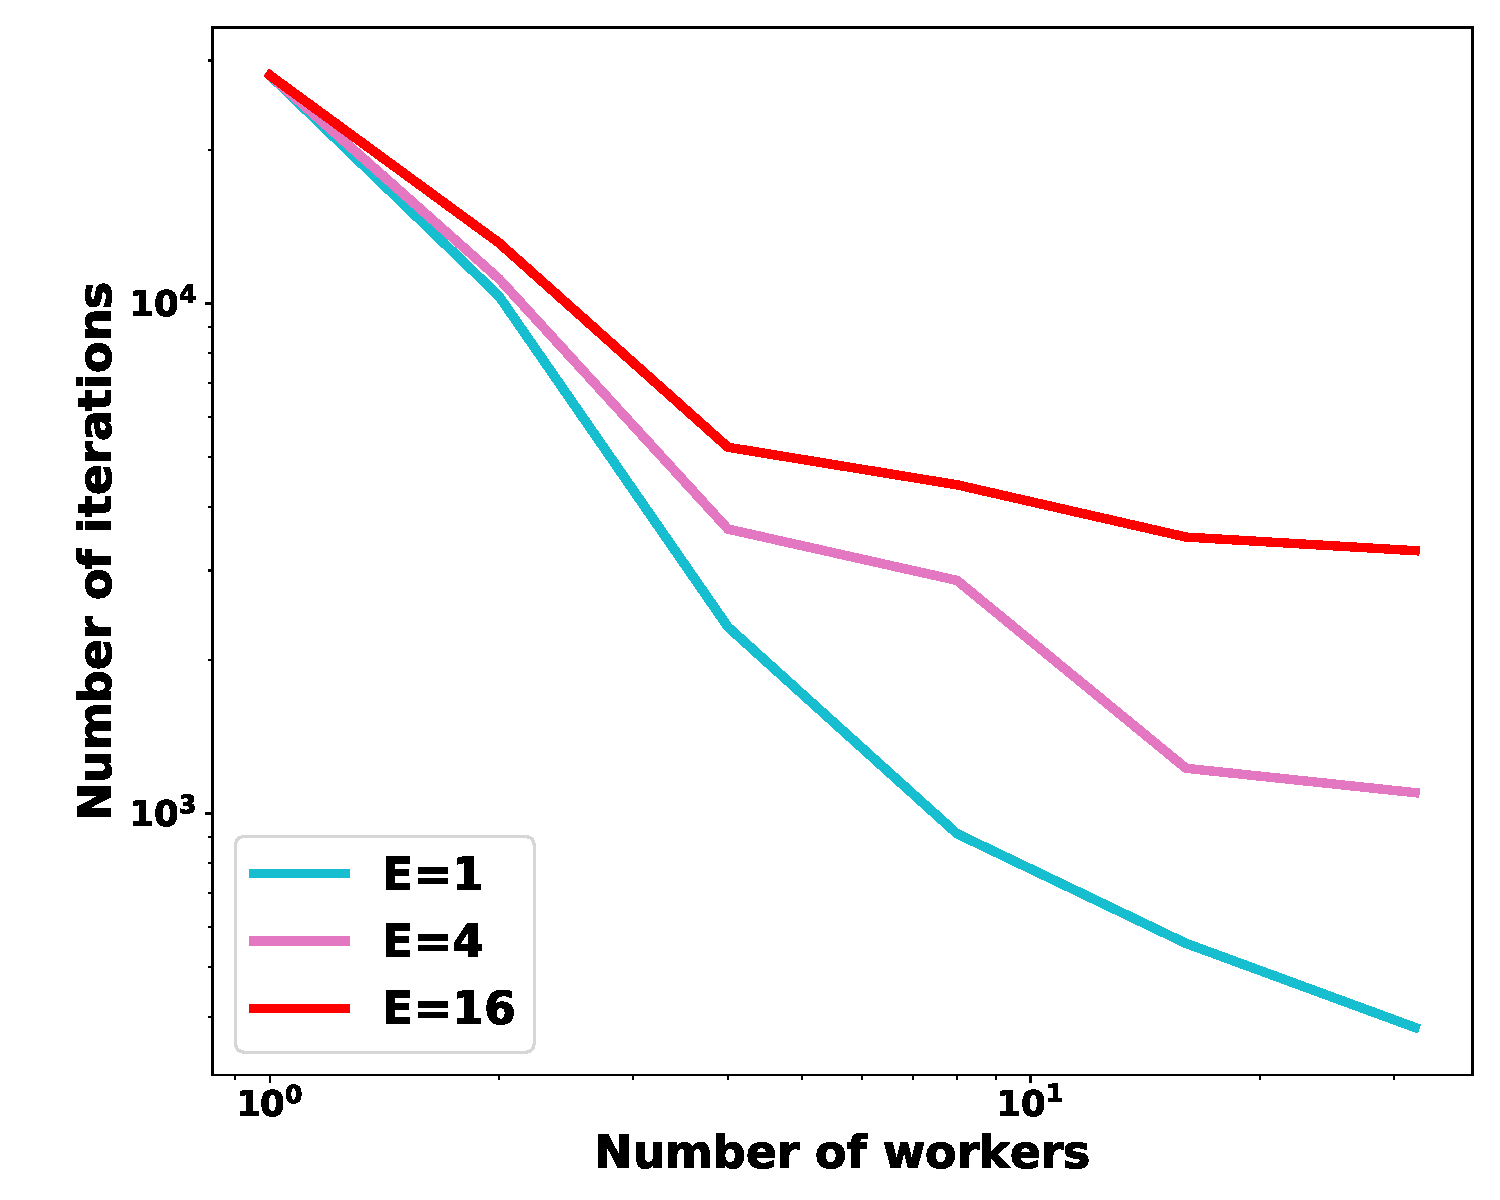
\includegraphics[width=0.33\textwidth]{fig/paper-stronglycvxsmthspeedupNodesT-min-w8a-epsilon0131-reg1e-05.pdf} &
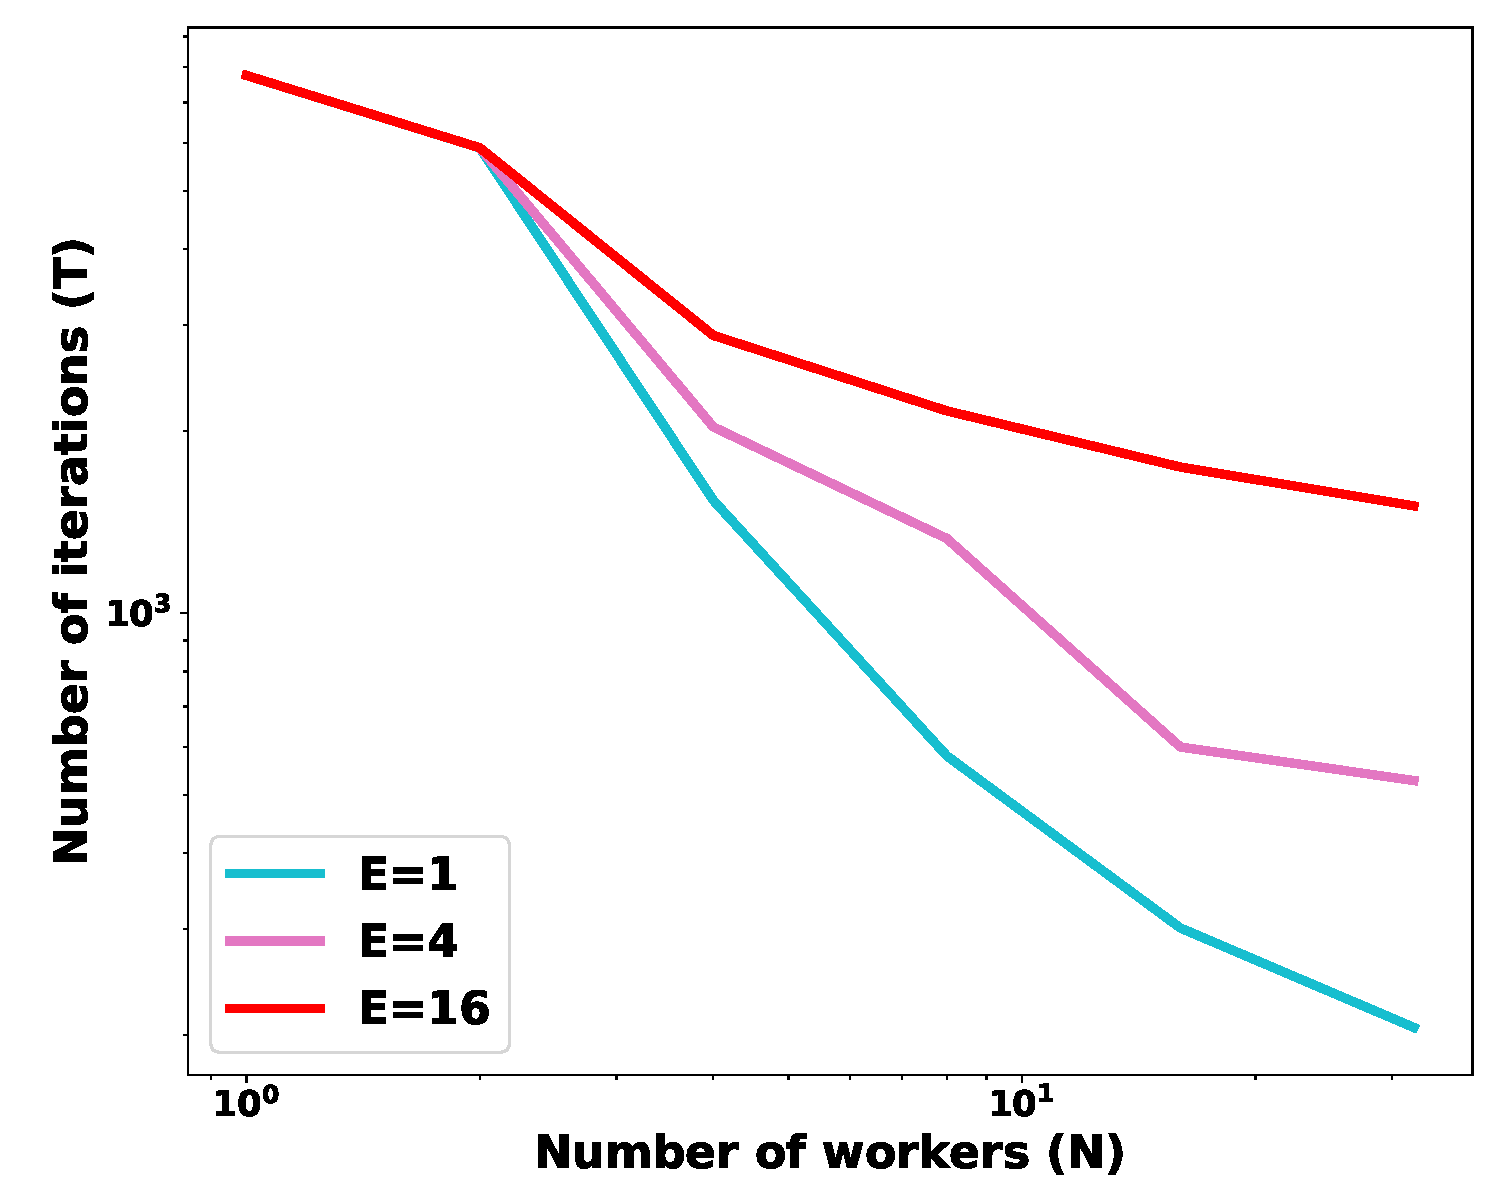
\includegraphics[width=0.33\textwidth]{fig/paper-cvxsmoothspeedupNodesT-min-w8a-epsilon0134-reg0.pdf} &
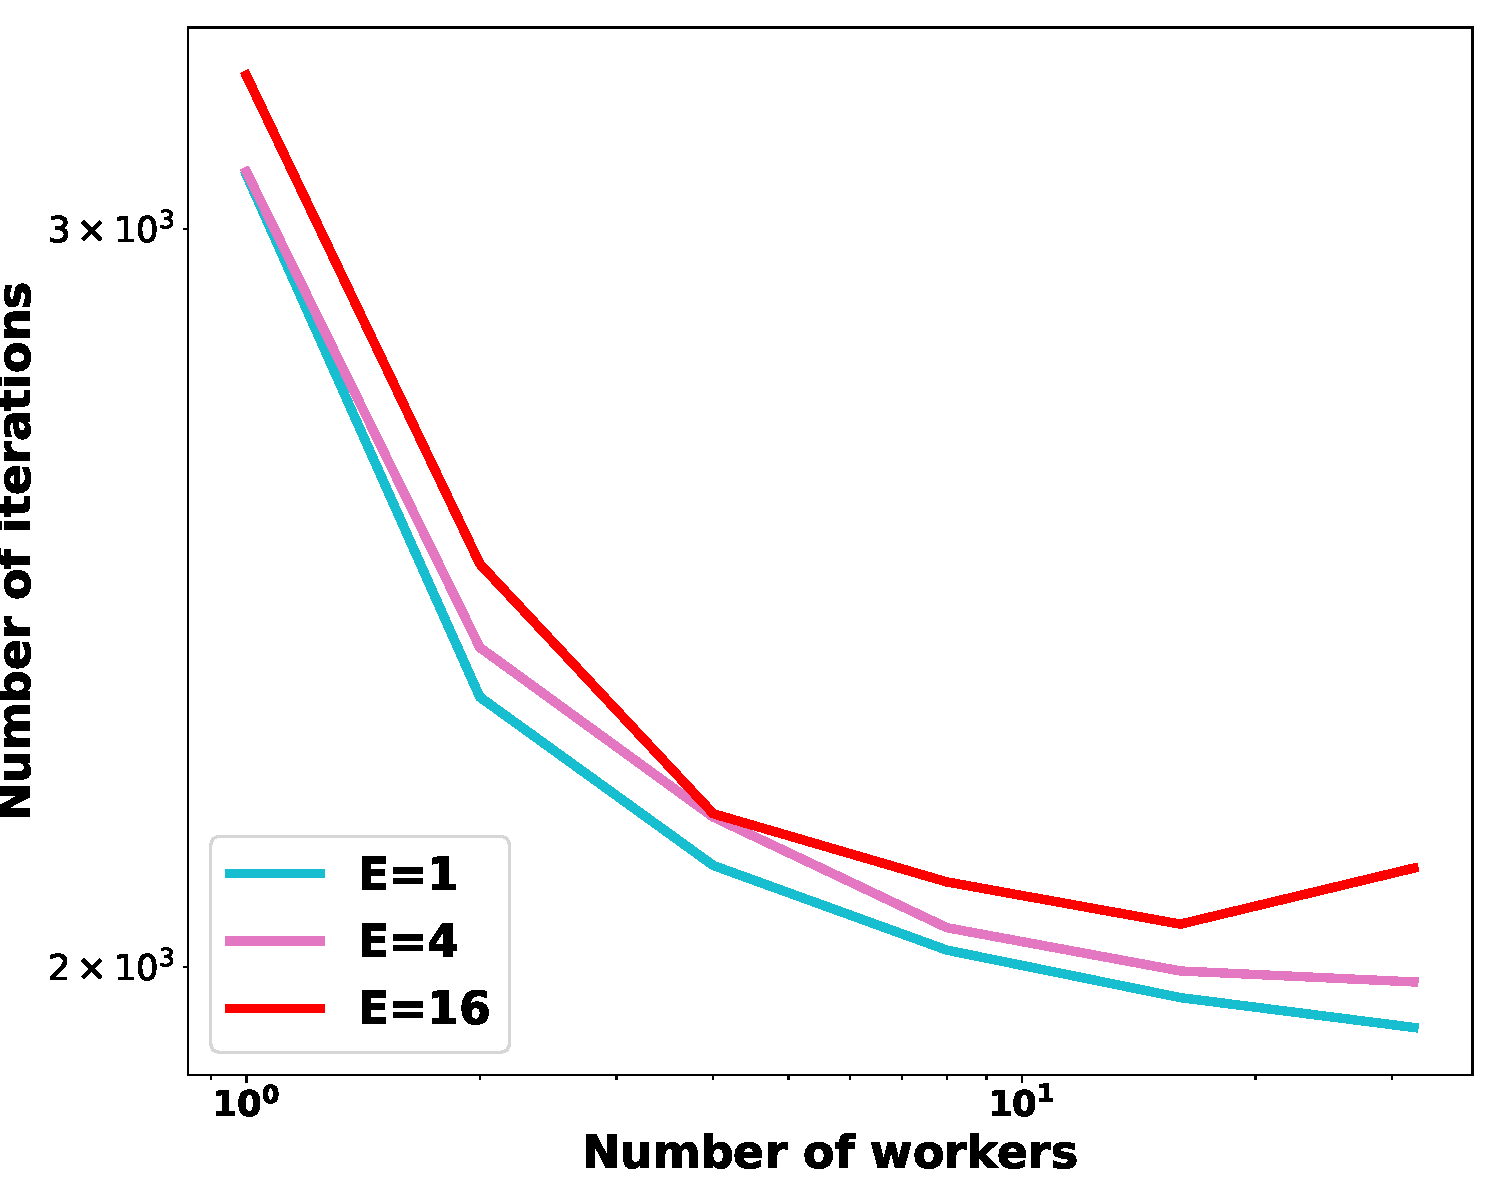
\includegraphics[width=0.33\textwidth]{fig/paper-linregressionspeedupNodesT-min-linearregressionw8a-epsilon002-reg0.pdf}\\
(a) Strongly convex objective & (b) Convex smooth objective & (c) Linear regression
	\end{tabular}
\caption{The linear speedup convergence of FedAvg w.r.t the number of workers. }
\label{fig:speedup}
\end{figure}

\begin{figure}
\centering
	\begin{tabular}{ccc}
	\hspace{-2em} 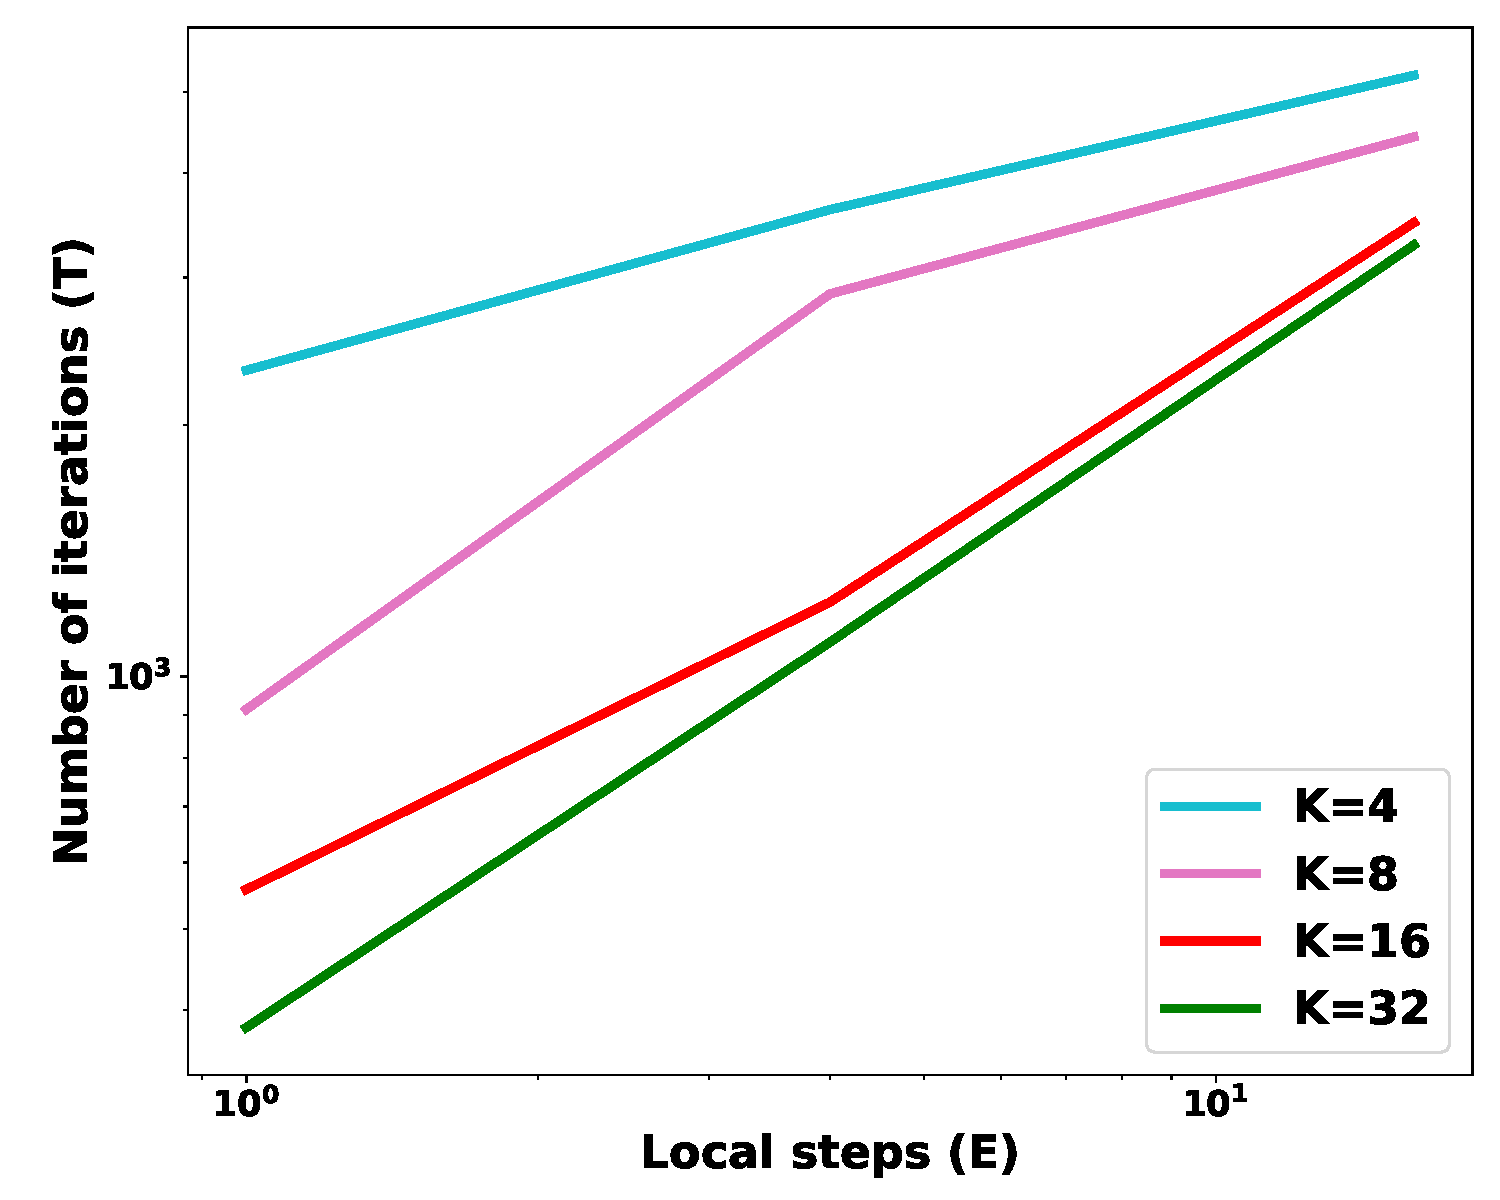
\includegraphics[width=0.33\textwidth]{fig/paper-stronglycvxsmthspeedupEpochsT-min-w8a-epsilon0131-reg1e-05.pdf} &
	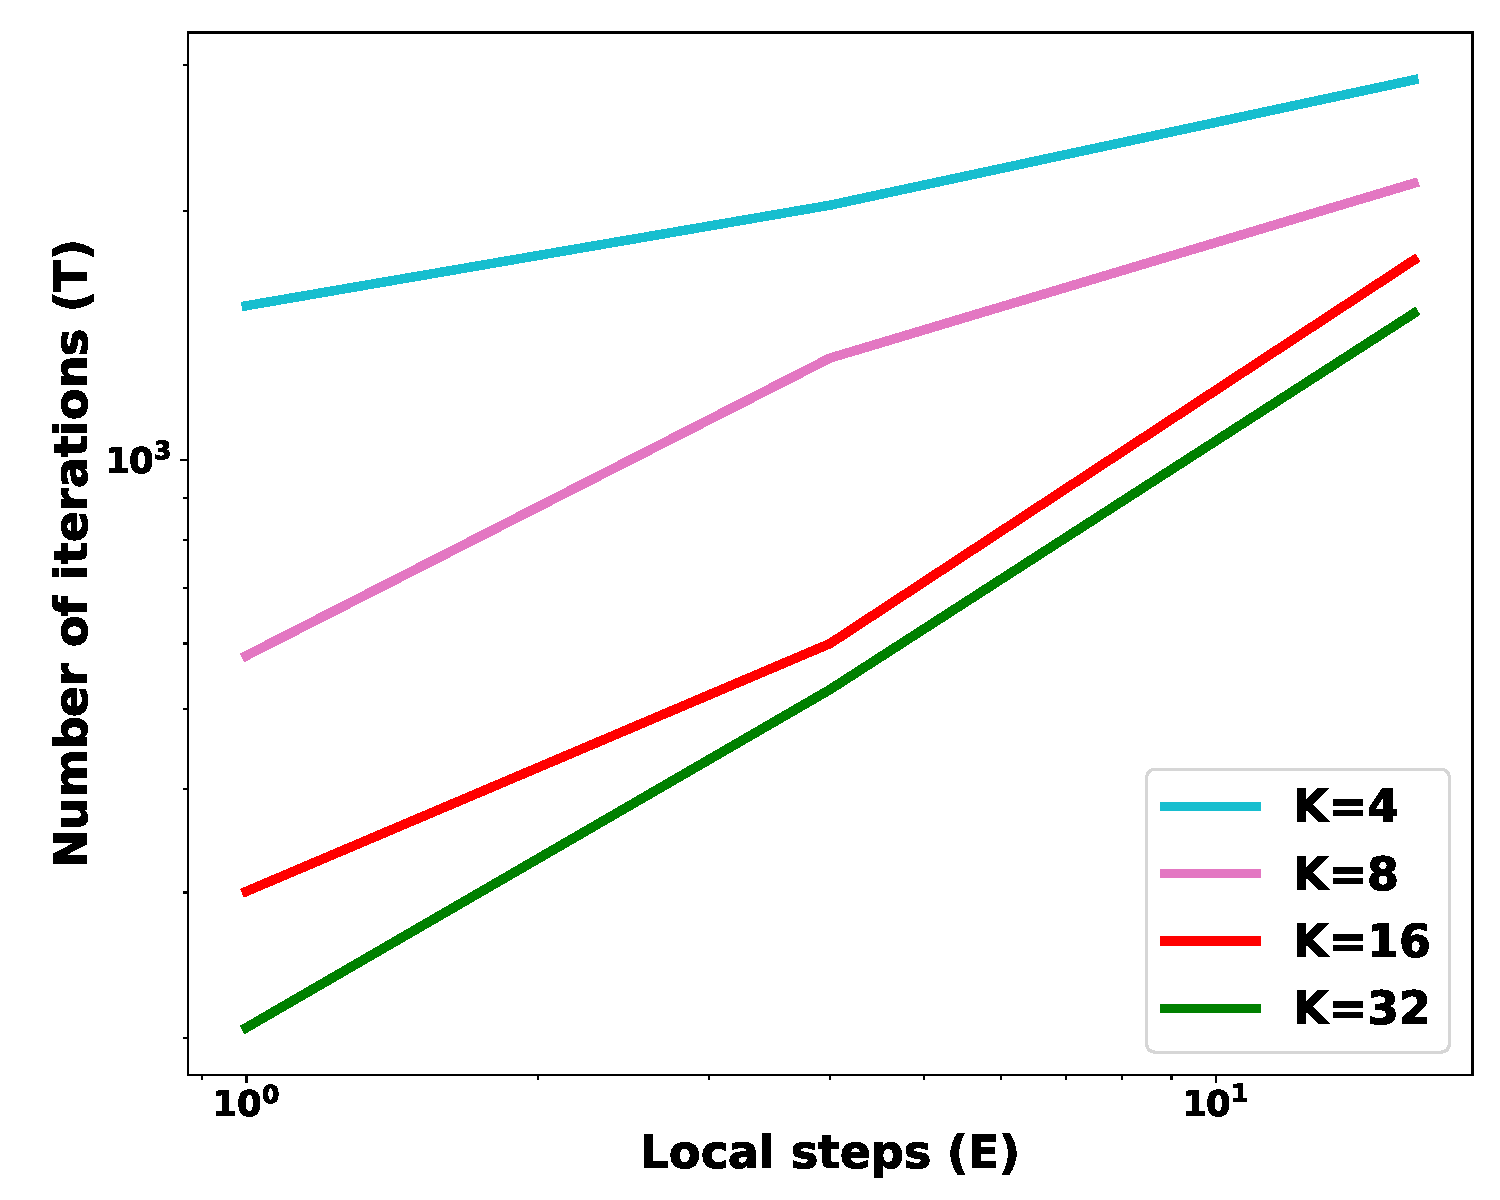
\includegraphics[width=0.33\textwidth]{fig/paper-cvxsmoothspeedupEpochsT-min-w8a-epsilon0134-reg0.pdf} & 
	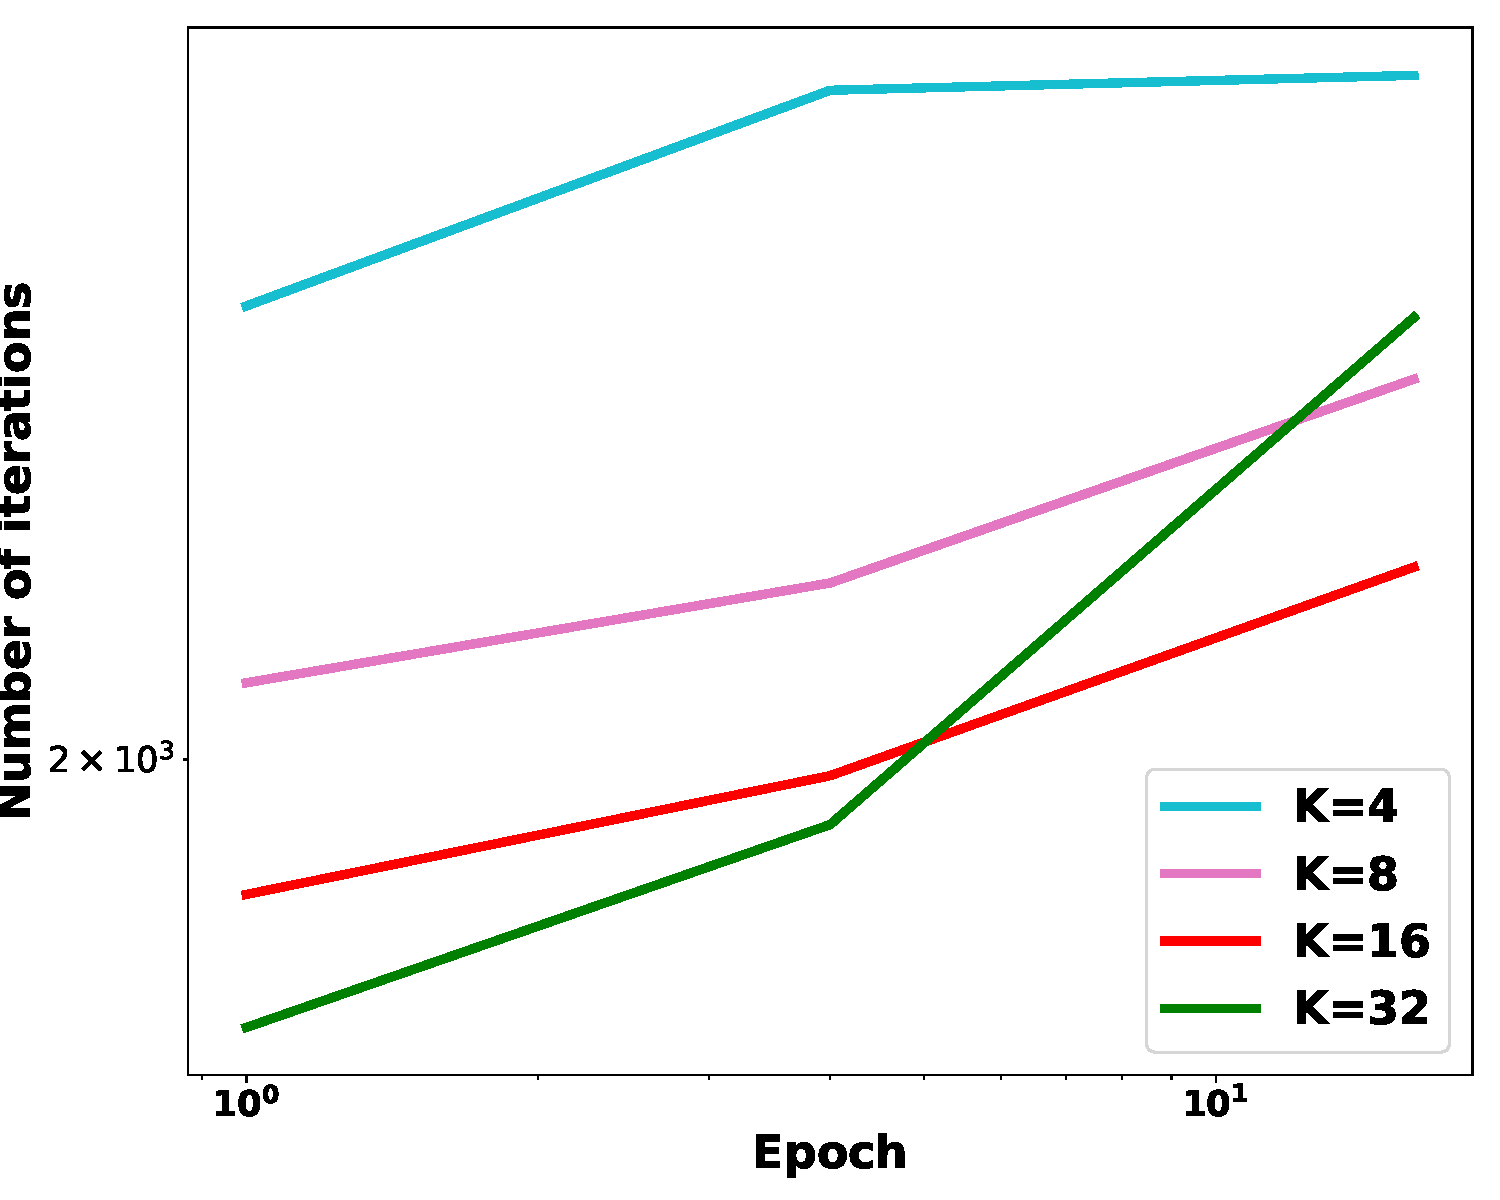
\includegraphics[width=0.33\textwidth]{fig/paper-linregressionspeedupEpochsT-min-linearregressionw8a-epsilon002-reg0.pdf} \\
	\hspace{-2em} 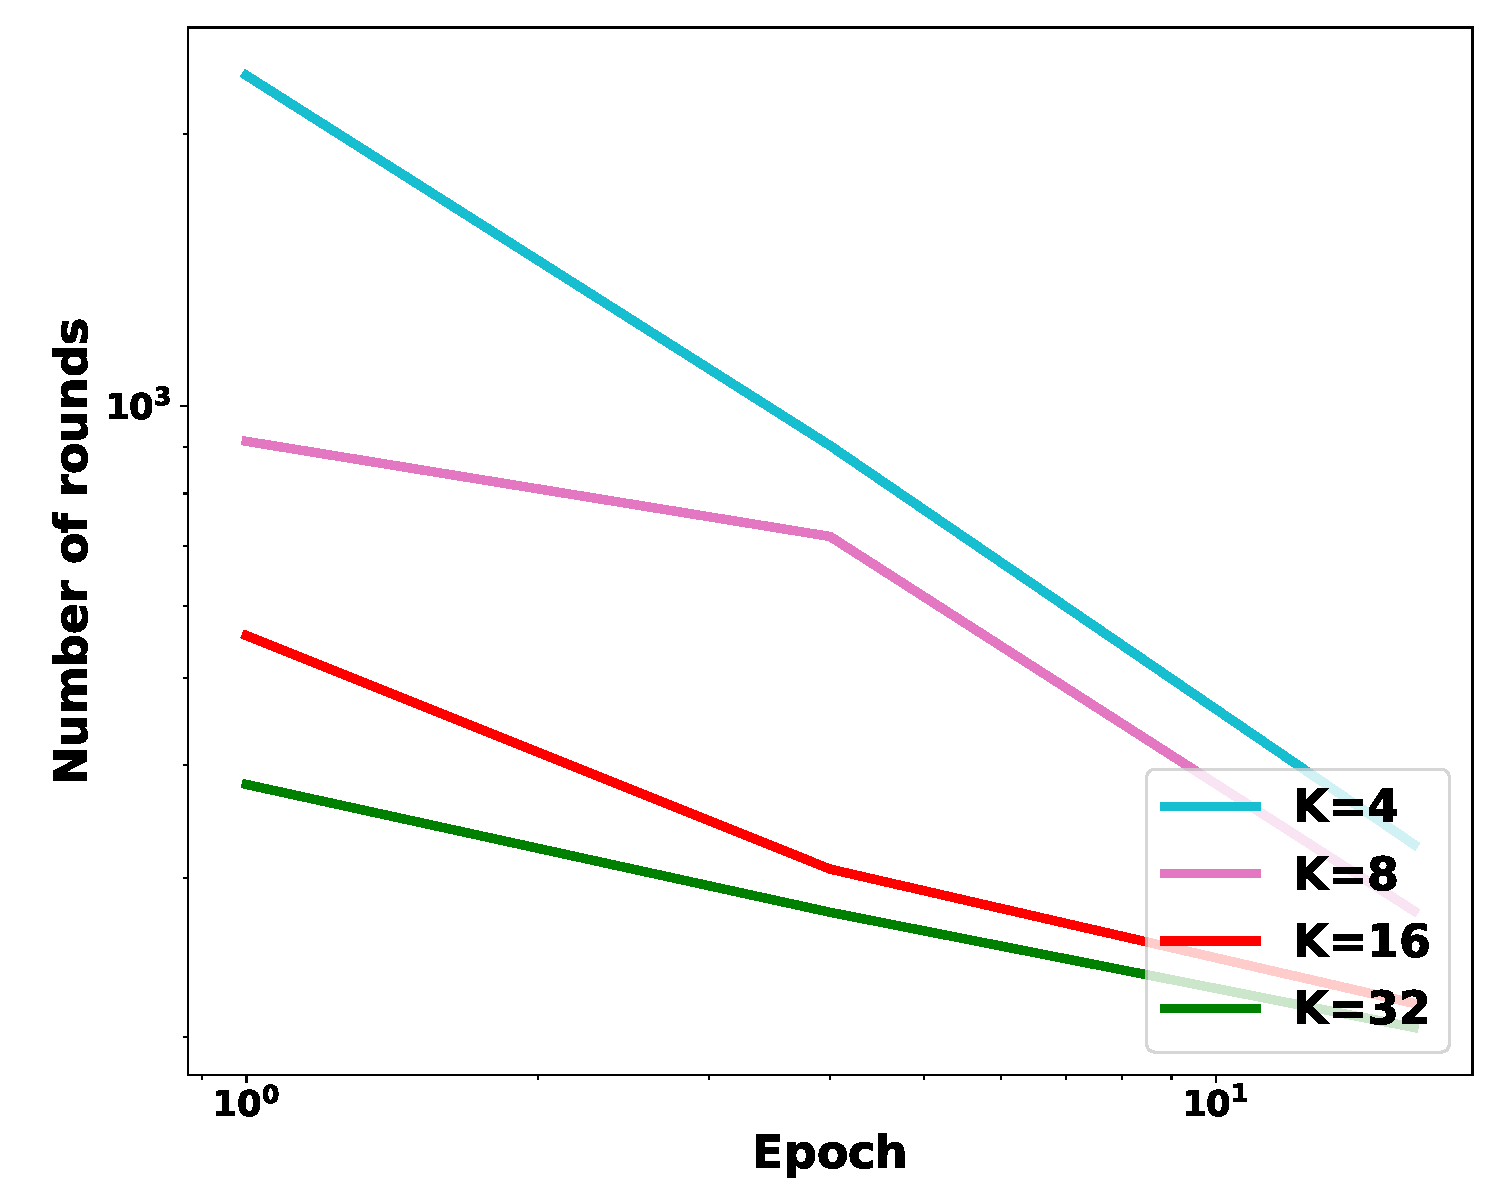
\includegraphics[width=0.33\textwidth]{fig/paper-stronglycvxsmthspeedupEpochsRounds-min-w8a-epsilon0131-reg1e-05.pdf} &
	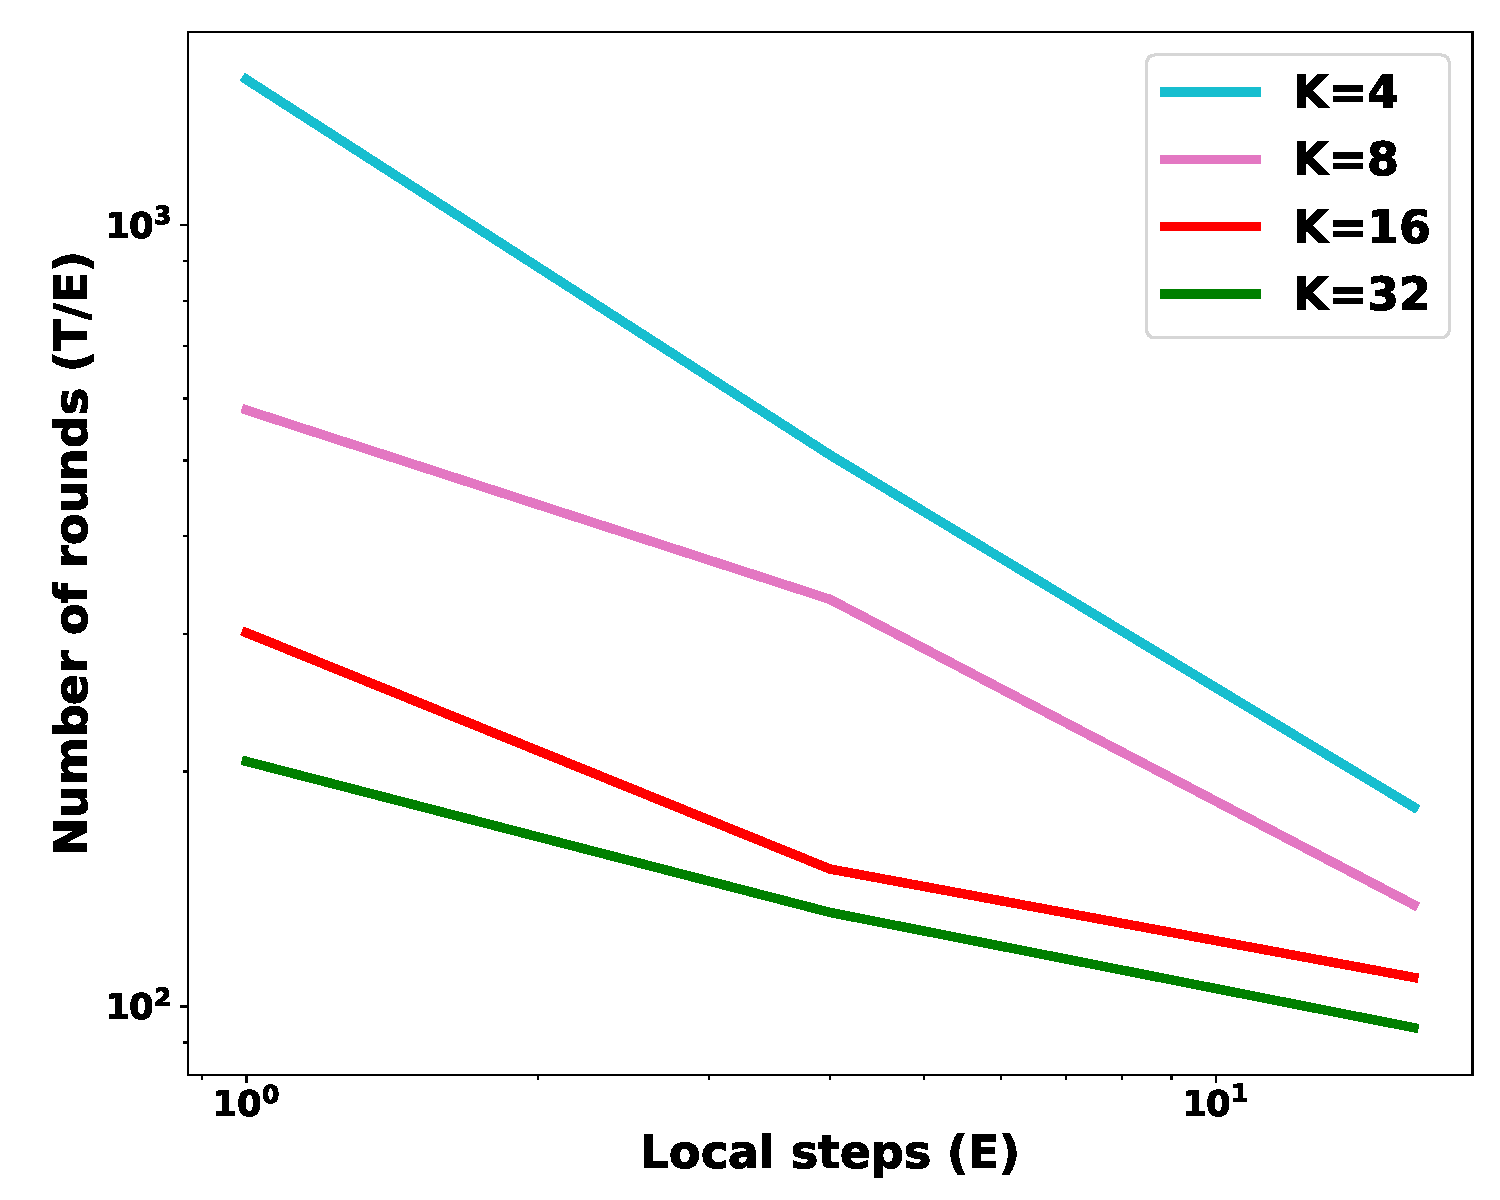
\includegraphics[width=0.33\textwidth]{fig/paper-cvxsmoothspeedupEpochsRounds-min-w8a-epsilon0134-reg0.pdf} & 
	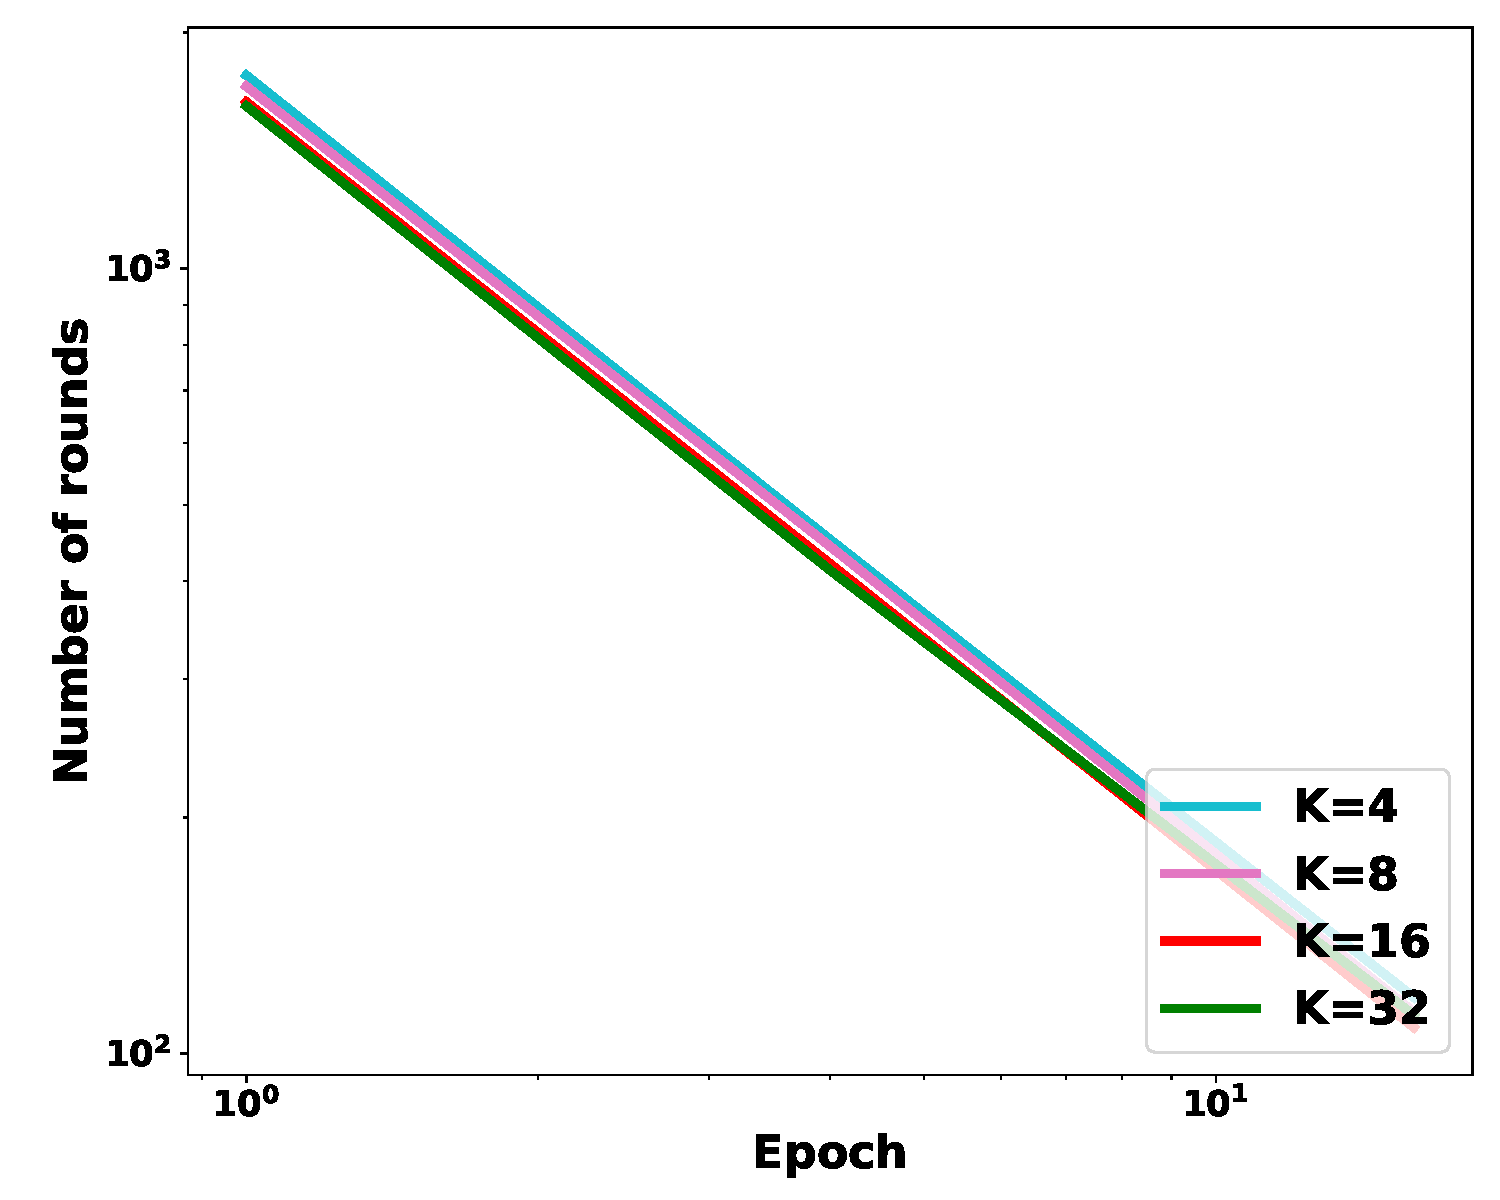
\includegraphics[width=0.33\textwidth]{fig/paper-linregression-newspeedupEpochsRounds-min-linearregressionw8a-epsilon002-reg0.pdf} \\
(a) Strongly convex objective & (b) Convex smooth objective & (c) Linear regression
	\end{tabular}
\caption{The convergence of FedAvg w.r.t the number of epochs. }
\label{fig:e}
\end{figure}

\begin{figure}
\centering
	\begin{tabular}{ccc}
	\hspace{-2em}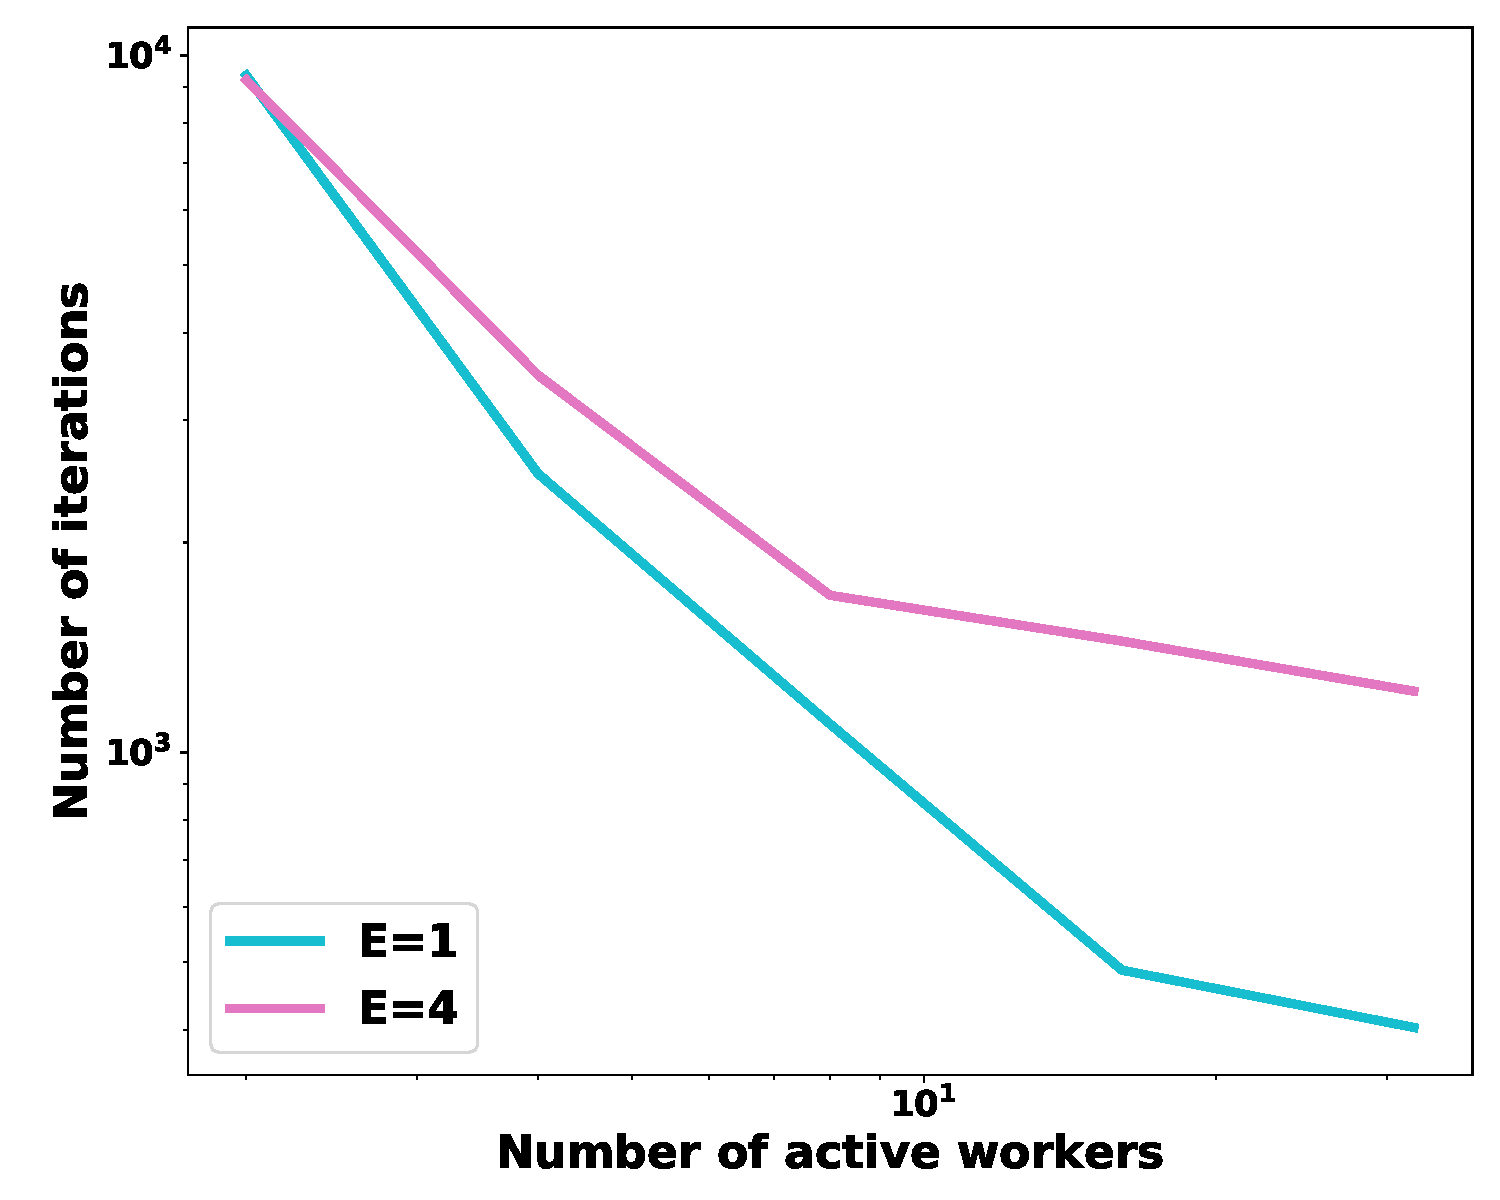
\includegraphics[width=0.33\textwidth]{fig/paper-partialstronglycvxsmthspeedupNodesT-min-w8a-epsilon0131-reg1e-05.pdf} &
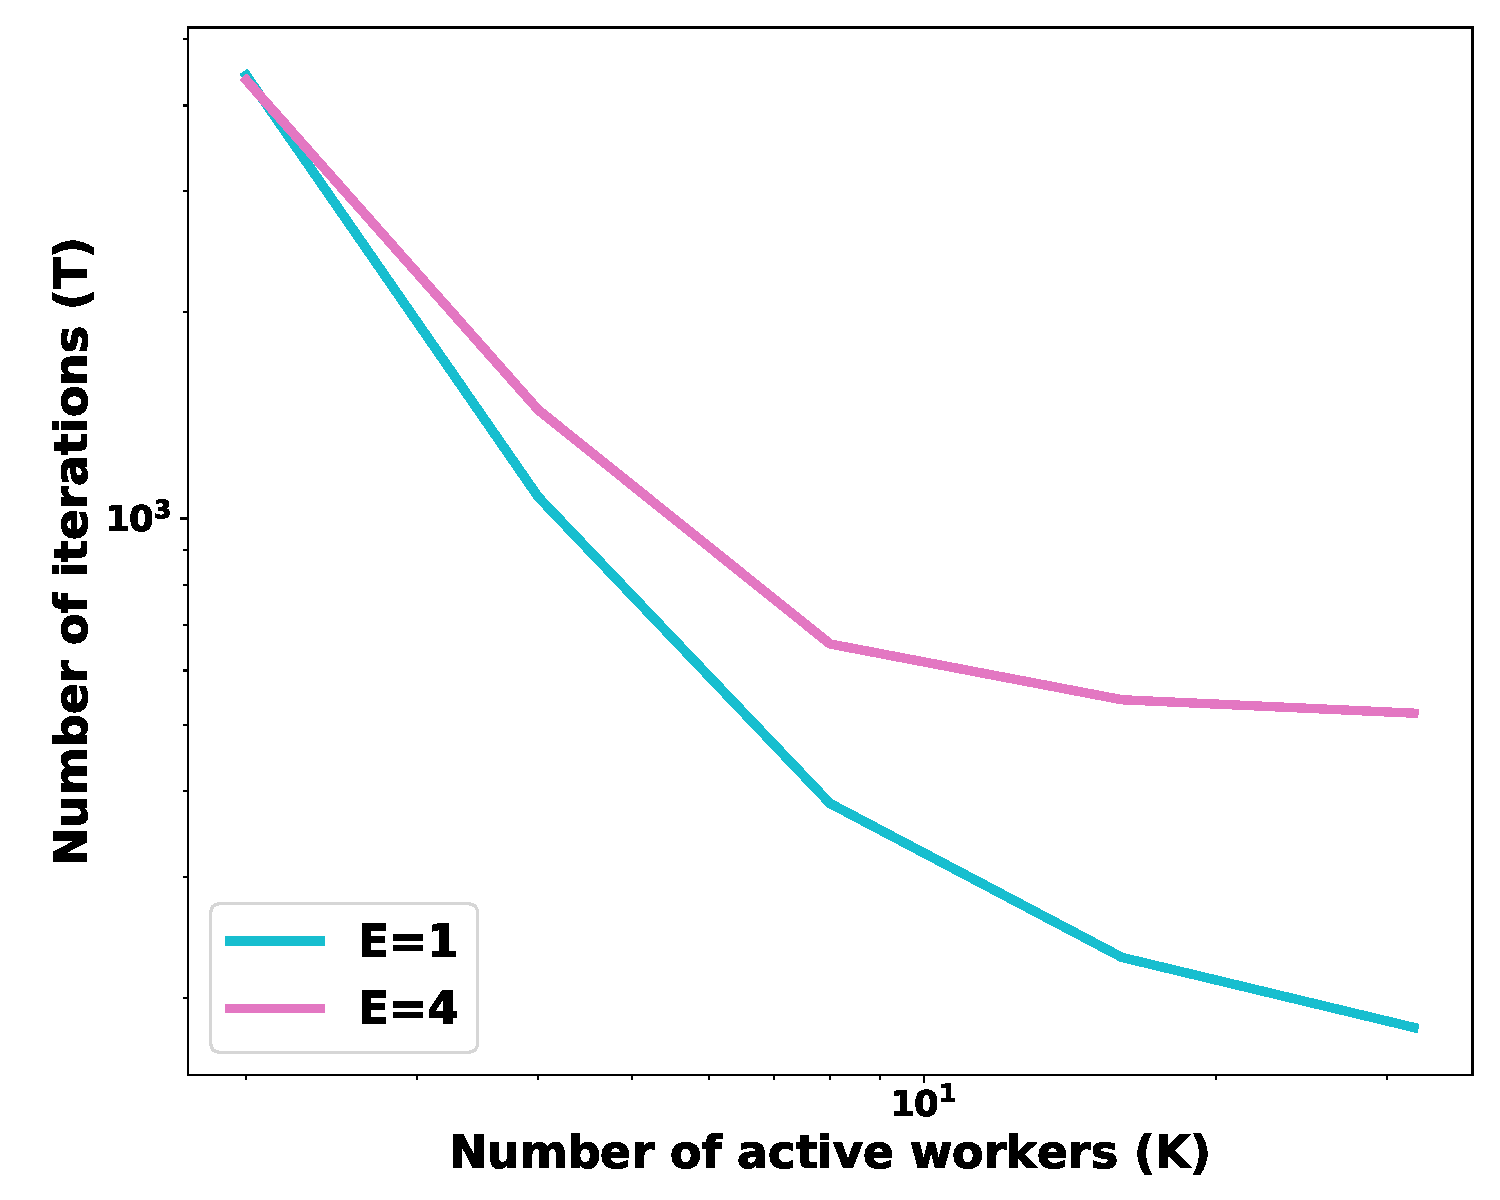
\includegraphics[width=0.33\textwidth]{fig/paper-partialcvxsmoothspeedupNodesT-min-w8a-epsilon0134-reg0.pdf} &
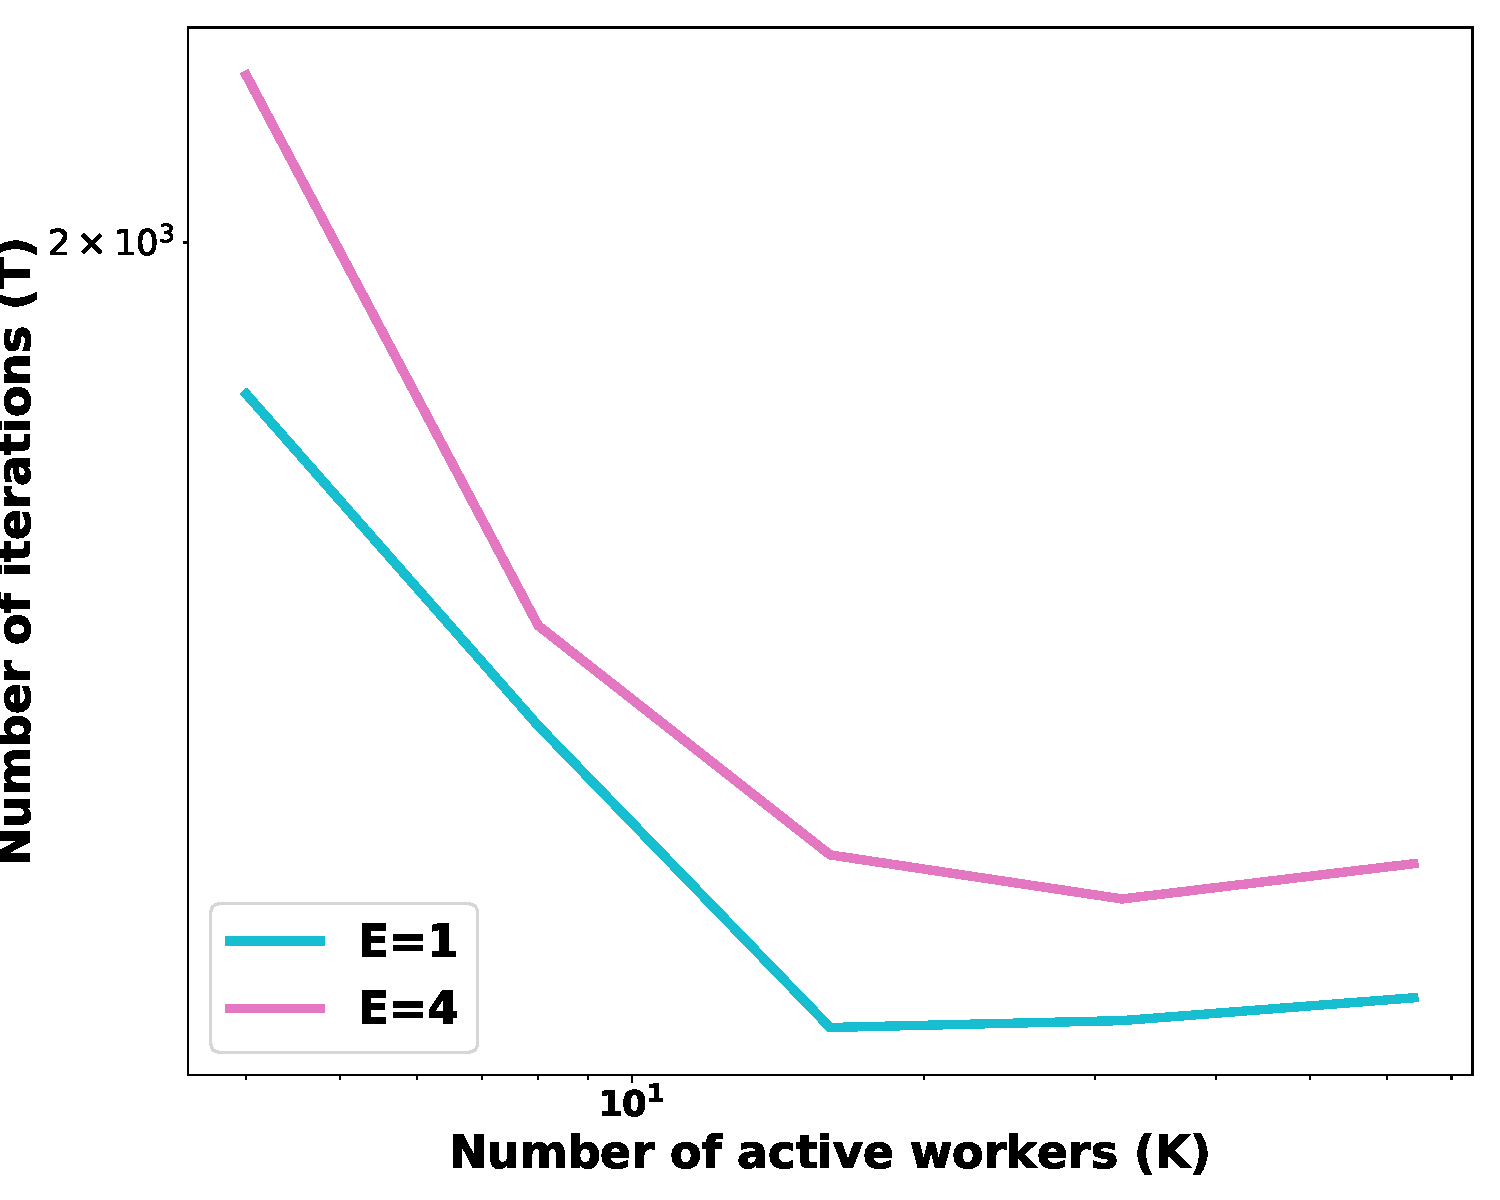
\includegraphics[width=0.33\textwidth]{fig/paper-partiallinregressionspeedupNodesT-min-linearregressionw8a-epsilon002-reg0.pdf}\\
(a) Strongly convex objective & (b) Convex smooth objective & (c) Linear regression
	\end{tabular}
\caption{The linear speedup convergence of FedAvg w.r.t the number of active workers. }
\label{fig:partial}
\end{figure}


\begin{figure}
\centering
\begin{tabular}{ccc}
\hspace{-2em}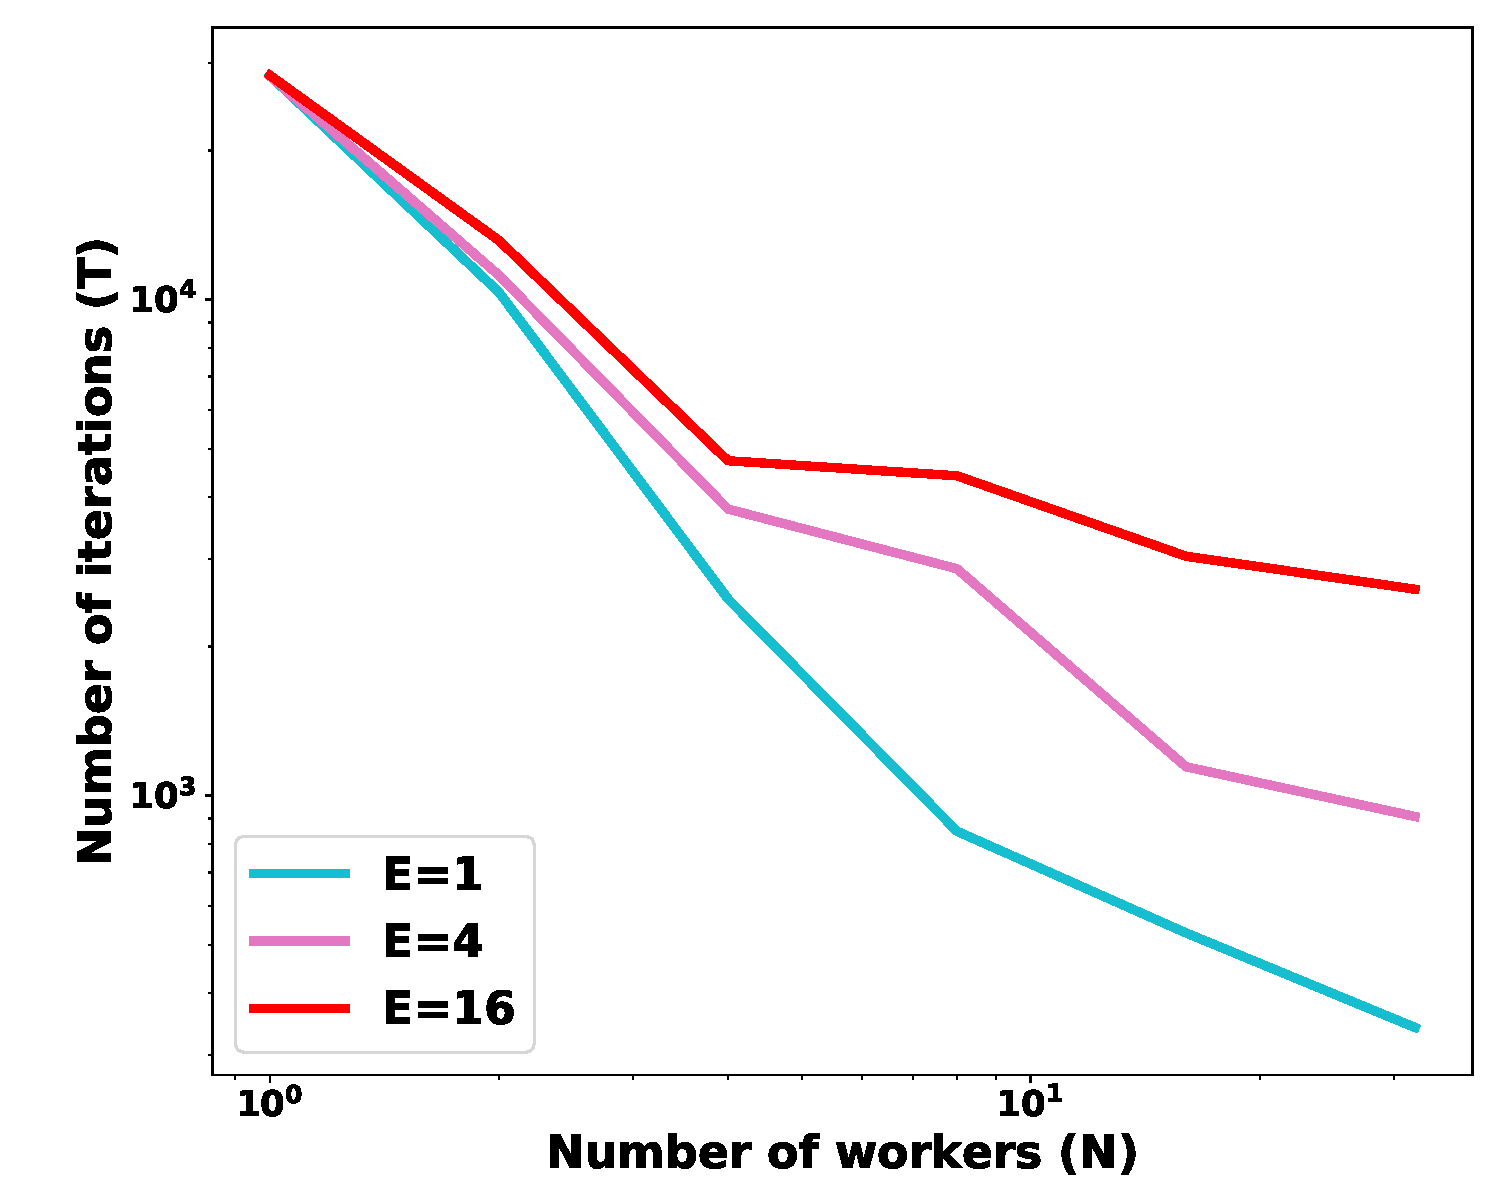
\includegraphics[width=0.33\textwidth]{fig/paper-nesterovspeedupNodesT-min-w8a-epsilon0131-reg1e-05.pdf} & 
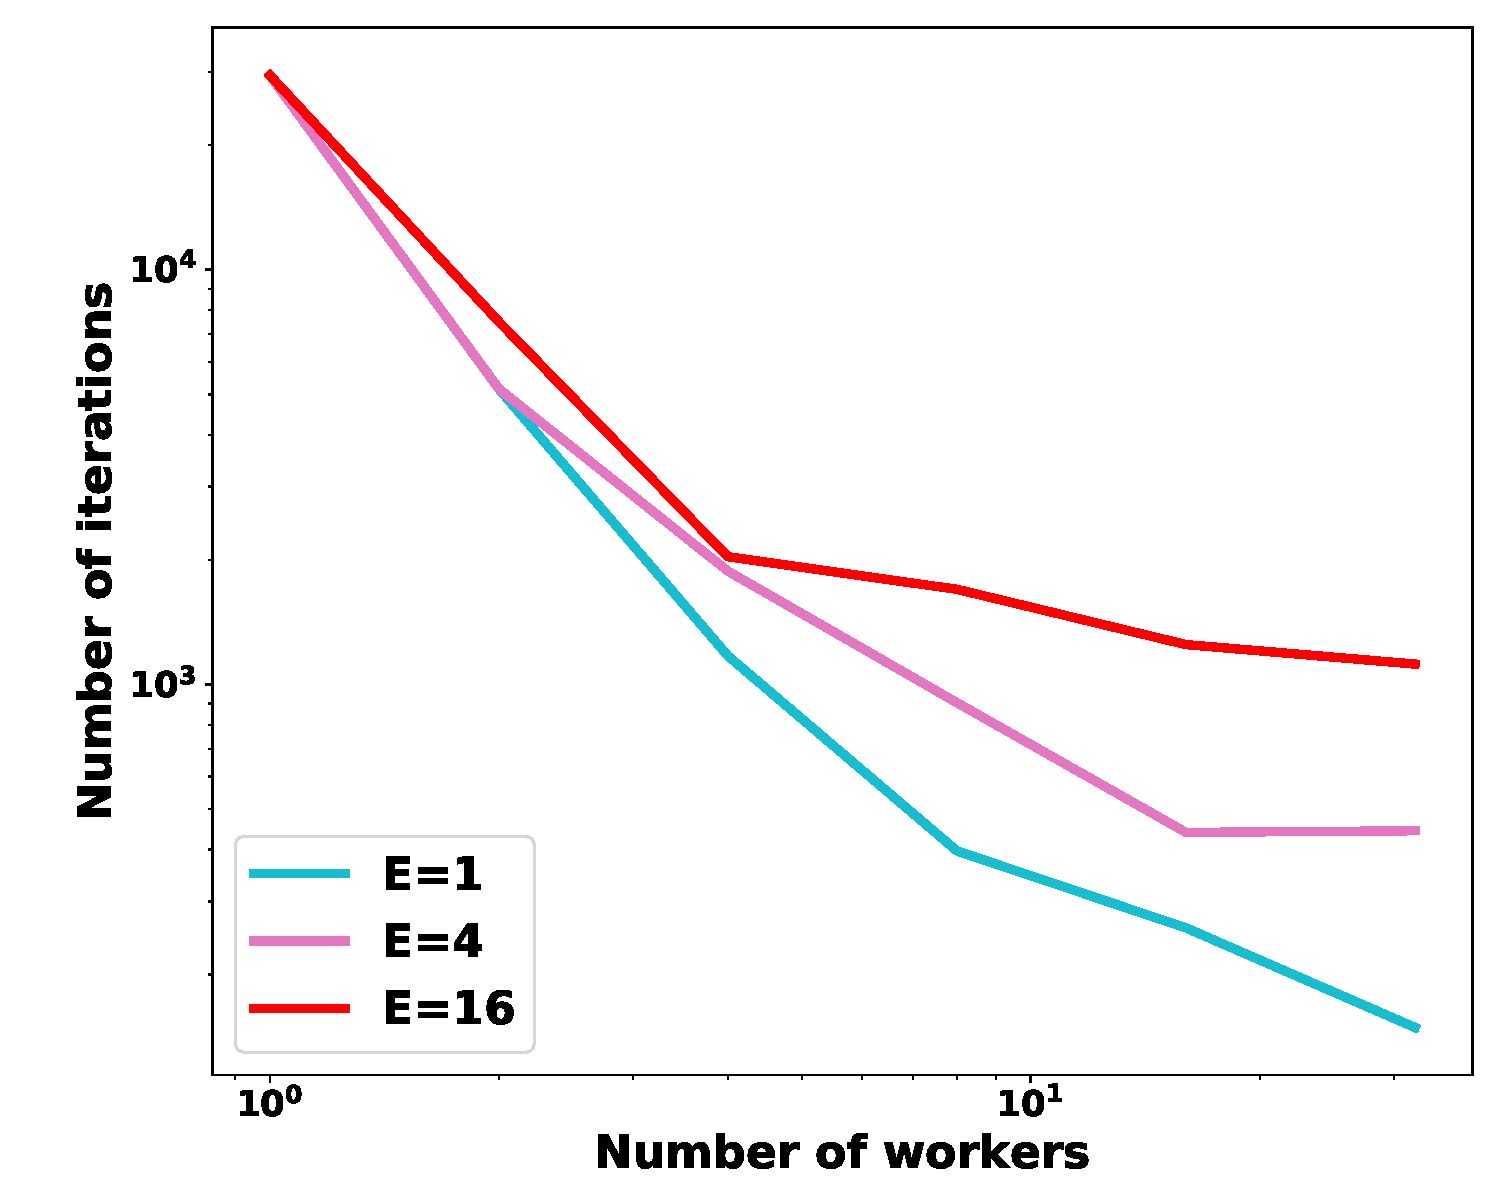
\includegraphics[width=0.33\textwidth]{fig/paper-nesterovspeedupNodesT-min-w8a-epsilon0134-reg0.pdf}
& 
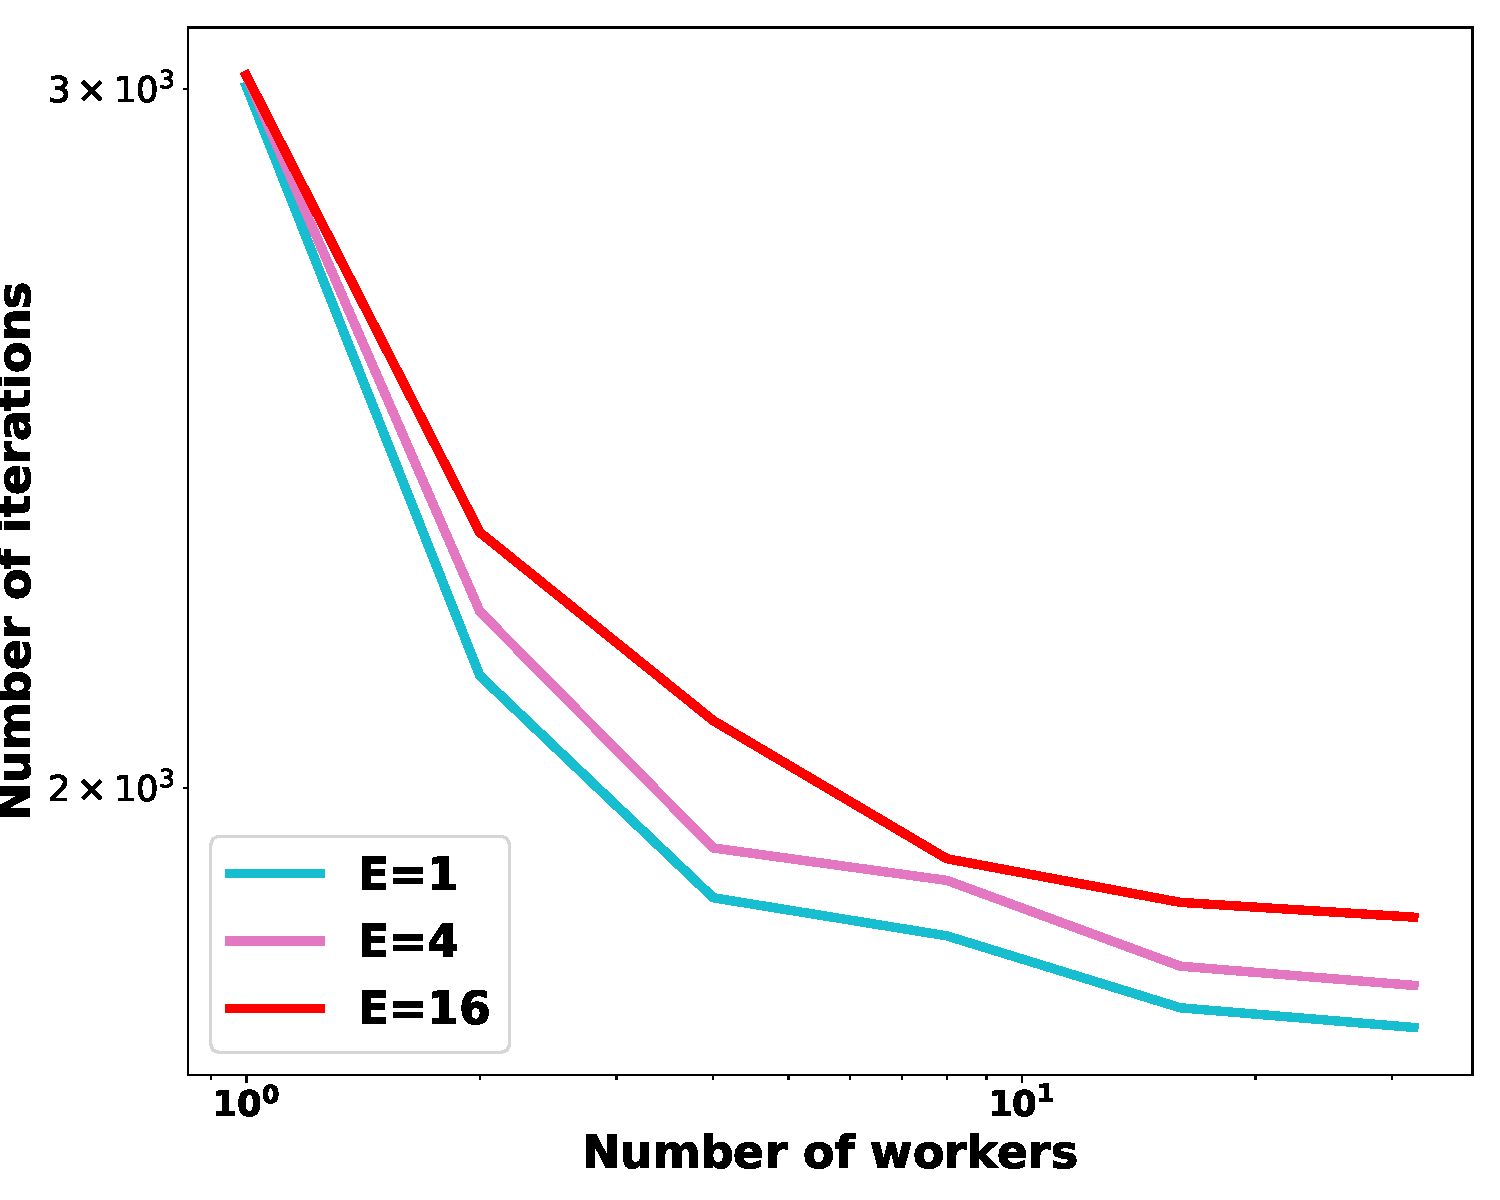
\includegraphics[width=0.33\textwidth]{fig/paper-lrnesterovspeedupNodesT-min-linearregressionw8a-epsilon002-reg0.pdf}\\
(a) Strongly convex objective & (b) Convex smooth objective & (c) Linear regression
	\end{tabular}
\caption{The linear speedup convergence of Nesterov accelerated FedAvg w.r.t the number of workers. }
\label{fig:nesterov}
\end{figure}



\newpage
\appendix
% !TEX ROOT=./main.tex





\section{Stochastic Gradient decent}

% 	Stochastic gradient of device $k$ at time step $t$, at point $\vw_t^k$: $$\vg_{t,k} \coloneqq \vg_{t,k}(w_t^k)$$
% 	$$ \vg_{t, k} = \grad F_{k}\left(w_{t}^{k}, \xi_{t}^{k}\right) $$
% 	$$\EE \vg_{t, k} = \grad F_{k}\left(w_{t}^{k}\right)$$
%   One-step stochastic subgradient of all devices.
% $$\vg_{t}=\sum_{k=1}^{N} p_{k} \vg_{t, k}\left(w_{t}^{k}\right) $$
% \begin{align}
% 	\EE \vg_{t}= \EE \sum_{k=1}^{N} p_{k} \vg_{t, k}\left(w_{t}^{k}\right) \coloneqq \sum_{k=1}^{N} p_{k} \EE \vg_{t, k}
% 	\label{eq:egtsgd}
% \end{align}


\subsection{Stochastic gradient descent}
\subsubsection{Convex}
\label{sec:convexsmoothsgd}
% !TEX ROOT=./main.tex


\textbf{Full Device Participation}

\begin{itemize}
	\item Stochastic gradient of device $k$ at time step $t$, at point $w_{t,k}$: 
	$$\vg_{t,k} \coloneqq \vg_{t,k}(w_t^k)$$
	$$ \vg_{t, k} = \grad F_{k}\left(w_{t}^{k}, \xi_{t}^{k}\right) $$
	$$\EE \vg_{t, k} = \grad F_{k}\left(w_{t}^{k}\right)$$
\item  One-step stochastic subgradient of all devices.
$$\vg_{t}=\sum_{k=1}^{N} p_{k} \vg_{t, k}\left(w_{t}^{k}\right) $$
\begin{align}
	\EE \vg_{t}= \EE \sum_{k=1}^{N} p_{k} \vg_{t, k}\left(w_{t}^{k}\right) \coloneqq \sum_{k=1}^{N} p_{k} \EE \vg_{t, k}
	\label{eq:egtsgd}
\end{align}
\end{itemize}



$$\Delta_{t+1} = \EE \|\overline{\vw}_{t+1} - \vw^*\|^2 = \EE \|\overline{\vv}_{t+1} - \vw^*\|^2,$$
According to the definition of $\overline{\vv}_{t+1}$ in \eq{\ref{eq:vbar}}, we can expand $\Delta_{t+1}$
$$\begin{aligned}\left\|\bar{\vv}_{t+1}-\vw^{*}\right\|^2 &=\left\|\ov{w}_{t}-\eta_{t} \vg_{t}-\vw^{*}\right\|^2 \\ &=\left\|\ov{w}_{t}-\vw^{*}\right\|^{2}-2 \eta_{t} \vg_{t}^{\top}\left(\ov{w}_{t}-\vw^{*}\right)+\eta_{t}^{2}\left\|\vg_{t}\right\|^{2} \end{aligned}$$

Take the expectation condition on $\vw_t$ over random samples at all devices:
\begin{align}
\Delta_{t+1} = \EE\left[\left\|\bar{\vv}_{t+1}-\vw^{*}\right\|^2| \vw_{t}\right]=\|\ov{w}_{t}-\vw^{*}\|^{2}-2 \eta_{t} \EE \vg_{t}^{\top}\left(\ov{w}_{t}-\vw^{*}\right)+\eta_{t}^{2} \EE\| \vg_{t} \|^{2}	
\label{eq:expandsgd}
\end{align}

Now we focus on bounding $-2 \eta_{t} \EE \vg_{t}^{\top}\left(\ov{w}_{t}-\vw^{*}\right)$ in \eq{\ref{eq:expandsgd}}: 

\begin{align*}
	& -2 \eta_{t} \left<\EE \vg_{t}, \ov{w}_{t}-\vw^{*}\right> \\
 =  & -2 \eta_{t} \left<\EE \vg_{t}, \ov{w}_{t}- \vw^{k}_t \right> -2 \eta_{t} \left<\EE \vg_{t}, \vw^{k}_t - \vw^{*}\right>\\
 \leq & -2 \eta_{t} \left<\EE \vg_{t}, \ov{w}_{t}- \vw^{k}_t \right> + 2 \eta_{t} (F_k(w^*) - F_k(\vw^{k}_t))\\
 \leq &\sum_{k=1}^N p_k \left[2 \eta_{t} (F_k(\vw^{k}_t) - F_k(\ov{w}_t) + \frac{L}{2} \|\ov{w}_t - \vw^{k}_t\|^2 ) + 2 \eta_{t} (F_k(w^*) - F_k(\vw^{k}_t))\right]\\
 = & \sum_{k=1}^N p_k \eta_t L \|\ov{w}_t - \vw^{k}_t\|^2 + 2 \eta_{t} \sum_{k=1}^N p_k (F_k(w^*) - F_k(\ov{w}_t))\\
 = &  \eta_t L \sum_{k=1}^N p_k \|\ov{w}_t - \vw^{k}_t\|^2 + 2 \eta_{t} (F^* - F(\ov{w}_t))
\end{align*}
Plug in this upper bound into \eq{\ref{eq:expandsgd}}, we have

\begin{align}
\EE\left\|\ov{w}_{t+1}-\vw^{*}\right\|^2 &\leq \|\ov{w}_{t}-\vw^{*}\|^{2}+\eta_{t}^{2} \EE\| \vg_{t} \|^{2} + \eta_t L \sum_{k=1}^N p_k \|\ov{w}_t - \vw^{k}_t\|^2 + 2 \eta_{t} (F^* - F(\ov{w}_t))\\
&\leq \|\ov{w}_{t}-\vw^{*}\|^{2}+\eta_{t}^{2} \EE\| \vg_{t} \|^{2} +  4L\eta_t^3(E-1)^2 G^2 + 2 \eta_{t} (F^* - F(\ov{w}_t))\\
&\leq \|\ov{w}_{t}-\vw^{*}\|^{2}+\eta_{t}^{2} G^2 +  4L\eta_t^3(E-1)^2 G^2 + 2 \eta_{t} (F^* - F(\ov{w}_t)) \label{eq:cvxsgd1}
\end{align}

Sum two sides of \eq{\ref{eq:cvxsgd1}}, we assume \lkxcom{$\eta_t < 1$}, set $F^*_t = \min_{t \in [0, T-1]} F(\ov{w}_t)$, 
\begin{align*}
	\sum_{t=0}^{T-1} 2\eta_t (F(\ov{w}_t) - F^* ) & \leq \EE \|\ov{w}_{0}-\vw^{*}\|^{2} - \EE\left\|\ov{w}_{T}-\vw^{*}\right\|^2 + \sum_{t=0}^{T-1} (\eta_t^3 4LG^2(E-1)^2 + \eta_t^2 G^2)\\ 
    & \leq \EE \|\ov{w}_{0}-\vw^{*}\|^{2} - \EE\left\|\ov{w}_{T}-\vw^{*}\right\|^2 + \sum_{t=0}^{T-1} (\eta_t^3 4LG^2(E-1)^2 + \eta_t^2 G^2)\\ 
    & \leq \EE \|\ov{w}_{0}-\vw^{*}\|^{2} + \sum_{t=0}^{T-1}\eta_t^2G^2 ( 4L(E-1)^2 + 1)\\
 F_t^* - F^*  & \leq \frac{\EE \|\ov{w}_{0}-\vw^{*}\|^{2}}{2 \sum_{t=0}^{T-1} \eta_t } + ( 4L(E-1)^2 + 1)G^2 \sum_{t=0}^{T-1} \eta_t^2
\end{align*}
It will converge under three conditions $ \lim_{T \rightarrow \infty }\sum_{t=0}^{T-1} \eta_t = \infty$
$ \lim_{T \rightarrow \infty }\sum_{t=0}^{T-1} \eta_t^2 < \infty$. For example, we can set $\eta_t = \frac{1}{t+1}$.


	
% % !TEX ROOT=./main.tex

Stochastic gradient of device $k$ at time step $t$, at point $\vw_t^k$: 
	$\vg_{t,k} \coloneqq \vg_{t,k}(w_t^k)$,
	$ \vg_{t, k} = \grad F_{k}\left(w_{t}^{k}, \xi_{t}^{k}\right) $,
	$\EE \vg_{t, k} = \grad F_{k}\left(w_{t}^{k}\right)$.
One-step stochastic gradient of all devices:
$\vg_{t}=\sum_{k=1}^{N} p_{k} \vg_{t, k}\left(w_{t}^{k}\right) $, $\EE \vg_{t}= \EE \sum_{k=1}^{N} p_{k} \vg_{t, k}\left(w_{t}^{k}\right) \coloneqq \sum_{k=1}^{N} p_{k} \EE \vg_{t, k} = \ov{g}_t$.

\begin{lemma}
Under Assumption~\ref{ass:subgrad2}, we have the following bound
\begin{equation}
	\eta_t^2 \|\EE \vg_{t,k}\|^2 \leq  \eta_t^2 G_k^2
	\label{eq:g3}
\end{equation}
\begin{equation}
	\eta_t^2 \|\EE \vg_{t,k}(\overline{\vw}_t)\|^2 \leq  \eta_t^2 G_k^2
	\label{eq:g2}
\end{equation}
\begin{align}
	  \eta_{t}^{2} \EE\| \vg_{t} \|^{2} 
	\leq   \eta_{t}^{2} \EE\| \sum_{k=1}^N p_k g_{t,k} \|^{2} 
	\leq   \eta_{t}^{2} \sum_{k=1}^N p_k \EE\| g_{t,k} \|^{2} 
	\leq   \eta_{t}^{2} \sum_{k=1}^N p_k G_k^2  \label{eq:g1}
\end{align}
\label{lma:gradient}
\end{lemma}


% Now the only term left in $C_1$ is $\eta_{t}^{2} \EE\| \vg_{t} \|^{2} $, follow the proof in Lemma 2~\cite{li2019convergence}:
% where in the third inequality we use the convexity of the l2 norm.

\begin{theorem}
Let Assumption~\ref{ass:subgrad2} and Assumption~\ref{ass:lsmooth} hold, suppose we have a bound 
on our starting distance, i.e., $\|\vw_{0} - \vw^*\|^2 \leq \Delta_0$, set learning rate $\eta_t =  \left(\frac{\Delta_0}{ T [G^2( 4L(E-1)^2 + 1) + C]}\right)^{1/2}$, we have,
$$\EE[ F_t^*] - F^*  \leq \left(\frac{ \Delta_0 [G^2( 4L(E-1)^2 + 1) + C] }{T}\right)^{1/2}$$
where we denote $F^*_t = \min_{t \in [0, T-1]} F(\ov{w}_t)$.
% \label{th:sgdcvxsmth}
\end{theorem}

\begin{proof}
	

\begin{align}
\EE_{\cS_{t+1}, \xi_{t}} \|\overline{\vw}_{t+1} - \vw^*\|^2 &= \EE_{\cS_{t+1}, \xi_{t}} \|\overline{\vw}_{t+1} - \overline{\vv}_{t+1} + \overline{\vv}_{t+1} - \vw^*\|^2\\
&= \EE_{\cS_{t+1}, \xi_{t}} \left[\|\overline{\vw}_{t+1} - \overline{\vv}_{t+1}\|^2 + \|\overline{\vv}_{t+1} - \vw^*\|^2\right] \\
& \hspace{3em}+ 2\EE_{\xi_{t}} \left<\EE_{\cS_{t+1}} \overline{\vw}_{t+1} - \overline{\vv}_{t+1},   \overline{\vv}_{t+1} - \vw^*\right> \\
& = \EE_{\cS_{t+1}, \xi_{t}} \|\overline{\vw}_{t+1} - \overline{\vv}_{t+1}\|^2 + \EE_{\xi_t} \|\overline{\vv}_{t+1} - \vw^*\|^2 \\
& \leq  \eta_t^2 C + \EE_{\xi_t} \|\overline{\vv}_{t+1} - \vw^*\|^2 \label{eq:sgdcvxsmth1}
\end{align}
where in the second line we use $\EE_{\cS_{t+1}} \overline{\vw}_{t+1}  = \overline{\vv}_{t+1}$. 
The first term can be bounded by consider different sampling scheme. 
According to the definition of $\overline{\vv}_{t+1}$ in \eq{\ref{eq:vbar}}, we can expand the second term in \eq{\ref{eq:sgdcvxsmth1}} as follows:

\begin{align*}
\left\|\ov{v}_{t+1}-\vw^{*}\right\|^2 
 &=\left\|\ov{w}_{t}-\eta_{t} \vg_{t}-\vw^{*}\right\|^2 \\
 &=\left\|\ov{w}_{t}-\vw^{*}\right\|^{2}-2 \eta_{t} \left< \vg_{t}, \ov{w}_{t}-\vw^{*} \right>+\eta_{t}^{2}\left\|\vg_{t}\right\|^{2} 
\end{align*}
% \begin{align*}
% \left\|\ov{v}_{t+1}-\vw^{*}\right\|^2 
%  &=\left\|\ov{w}_{t}-\eta_{t} \vg_{t}-\vw^{*}\right\|^2 \\
%  &=\left\|\ov{w}_{t}-\eta_{t} \vg_{t}-\vw^{*} - \eta_t \ov{g}_t + \eta_t \ov{g}_t\right\|^2 
% \\
% & = \left\|\ov{w}_{t}- \eta_t \ov{g}_t  -\vw^{*} + \eta_t \ov{g}_t - \eta_{t} \vg_{t}\right\|^2 \\
% & = \left\|\ov{w}_{t}- \eta_t \ov{g}_t  -\vw^{*}\right\|^2  + 2\eta_t \left<\vw_t - \vw^* - \eta_t \ov{g}_t, \ov{g}_t - \vg_{t} \right> + \left\|\eta_t \ov{g}_t - \eta_{t} \vg_{t}\right\|^2 \\
%  &=\left\|\ov{w}_{t}-\vw^{*}\right\|^{2}-2 \eta_{t} \left<\EE \vg_{t}, \ov{w}_{t}-\vw^{*} \right>+\eta_{t}^{2}\left\|\ov{g}_{t}\right\|^{2}  + \underbrace{2\eta_t \left<\vw_t - \vw^* - \eta_t \ov{g}_t, \ov{g}_t - \vg_{t} \right>}_{A_1} + \eta_{t}^2\left\| \ov{g}_t -  \vg_{t}\right\|^2
% \end{align*}

We take the expectation condition on $\vw_t$ over $\xi_t$, i.e., random samples at all devices:
\begin{align}
\EE\left[\left\|\ov{v}_{t+1}-\vw^{*}\right\|^2| \vw_{t}\right]=\|\ov{w}_{t}-\vw^{*}\|^{2}-2 \eta_{t} \left<\EE \vg_{t}, \ov{w}_{t}-\vw^{*} \right> +\eta_{t}^{2} \EE\| \vg_{t} \|^{2}
\label{eq:expandsgd}
\end{align}

Now we focus on bounding $-2 \eta_{t} \left< \EE \vg_{t}, \ov{w}_{t}-\vw^{*}\right>$ in \eq{\ref{eq:expandsgd}}: 

\begin{align*}
	& -2 \eta_{t} \left<\EE \vg_{t}, \ov{w}_{t}-\vw^{*}\right> \\
 =  & -2 \eta_{t} \left<\EE \vg_{t}, \ov{w}_{t}- \vw^{k}_t \right> -2 \eta_{t} \left<\EE \vg_{t}, \vw^{k}_t - \vw^{*}\right>\\
 \leq & -2 \eta_{t} \left<\EE \vg_{t}, \ov{w}_{t}- \vw^{k}_t \right> + 2 \eta_{t} (F_k(w^*) - F_k(\vw^{k}_t))\\
 \leq &\sum_{k=1}^N p_k \left[2 \eta_{t} (F_k(\vw^{k}_t) - F_k(\ov{w}_t) + \frac{L}{2} \|\ov{w}_t - \vw^{k}_t\|^2 ) + 2 \eta_{t} (F_k(w^*) - F_k(\vw^{k}_t))\right]\\
 = & \sum_{k=1}^N p_k \eta_t L \|\ov{w}_t - \vw^{k}_t\|^2 + 2 \eta_{t} \sum_{k=1}^N p_k (F_k(w^*) - F_k(\ov{w}_t))\\
 = &  \eta_t L \sum_{k=1}^N p_k \|\ov{w}_t - \vw^{k}_t\|^2 + 2 \eta_{t} (F^* - F(\ov{w}_t))
\end{align*}
Plug in this upper bound into \eq{\ref{eq:expandsgd}}, \eq{\ref{eq:sgdcvxsmth1}} and take totoal expectation over all samples at all iterations, we have
\begin{align}
\EE\left\|\ov{w}_{t+1}-\vw^{*}\right\|^2 &\leq \EE\|\ov{w}_{t}-\vw^{*}\|^{2}+\eta_{t}^{2} \EE\| \vg_{t} \|^{2} + \eta_t L \sum_{k=1}^N p_k \EE \|\ov{w}_t - \vw^{k}_t\|^2 + 2 \eta_{t} (F^* - \EE F(\ov{w}_t)) + \eta_t^2 C\\
&\leq\EE \|\ov{w}_{t}-\vw^{*}\|^{2}+\eta_{t}^{2} \EE\| \vg_{t} \|^{2} +  4L\eta_t^3(E-1)^2 G^2 + 2 \eta_{t} (F^* - \EE F(\ov{w}_t)) + \eta_t^2 C\\
&\leq \EE\|\ov{w}_{t}-\vw^{*}\|^{2}+\eta_{t}^{2} G^2 +  4L\eta_t^3(E-1)^2 G^2 + 2 \eta_{t} (F^* - \EE F(\ov{w}_t))+\eta_t^2 C \label{eq:cvxsgd1}
\end{align}

Sum two sides of \eq{\ref{eq:cvxsgd1}}, we require $\eta_t < 1$ and set $F^*_t = \min_{t \in [0, T-1]} F(\ov{w}_t)$, 
\begin{align*}
	\sum_{t=0}^{T-1} 2\eta_t (\EE[F(\ov{w}_t)] - F^* ) & \leq \EE \|\ov{w}_{0}-\vw^{*}\|^{2} - \EE\left\|\ov{w}_{T}-\vw^{*}\right\|^2 + \sum_{t=0}^{T-1} (\eta_t^3 4LG^2(E-1)^2 + \eta_t^2 G^2+ \eta_t^2 C)\\ 
    & \leq \EE \|\ov{w}_{0}-\vw^{*}\|^{2} - \EE\left\|\ov{w}_{T}-\vw^{*}\right\|^2 + \sum_{t=0}^{T-1} (\eta_t^3 4LG^2(E-1)^2 + \eta_t^2 G^2+ \eta_t^2 C)\\ 
    & \leq \EE \|\ov{w}_{0}-\vw^{*}\|^{2} + \sum_{t=0}^{T-1}\eta_t^2\left[ G^2 ( 4L(E-1)^2 + 1) + C\right]\\
    \sum_{t=0}^{T-1} 2\eta_t (\EE[F^*_t] - F^* ) & \leq \EE \|\ov{w}_{0}-\vw^{*}\|^{2} + \sum_{t=0}^{T-1}\eta_t^2\left[ G^2 ( 4L(E-1)^2 + 1) + C\right]\\
\EE[ F_t^*] - F^*  & \leq \frac{\|\ov{w}_{0}-\vw^{*}\|^{2}}{2 \sum_{t=0}^{T-1} \eta_t } + \frac{\left[G^2( 4L(E-1)^2 + 1) + C\right] \sum_{t=0}^{T-1} \eta_t^2}{2 \sum_{t=0}^{T-1} \eta_t }
\end{align*}
It will converge under the following conditions: $ \lim_{T \rightarrow \infty }\sum_{t=0}^{T-1} \eta_t = \infty$, 
$ \lim_{T \rightarrow \infty }\sum_{t=0}^{T-1} \eta_t^2 < \infty$. 
\begin{align*}
	\EE[ F_t^*] - F^*  & \leq \frac{\|\ov{w}_{0}-\vw^{*}\|^{2}}{2 \sum_{t=0}^{T-1} \eta_t } + \frac{\left[G^2( 4L(E-1)^2 + 1) + C\right] \sum_{t=0}^{T-1} \eta_t^2}{2 \sum_{t=0}^{T-1} \eta_t } \\
	\EE[ F_t^*] - F^*  & \leq \frac{\Delta_0 + \left[G^2( 4L(E-1)^2 + 1) + C\right] \sum_{t=0}^{T-1} \eta_t^2 }{2 \sum_{t=0}^{T-1} \eta_t }\\
	& \leq \left(\frac{ \Delta_0 [G^2( 4L(E-1)^2 + 1) + C] }{T}\right)^{1/2}
\end{align*}
where in the last line we set the learning rate satisfying $\eta_t =  \left(\frac{\Delta_0}{ T [G^2( 4L(E-1)^2 + 1) + C]}\right)^{1/2}$.
\end{proof}

% \subsubsection{Convex}
% \label{sec:sgdcvxnonsmth}
% !TEX ROOT=./main.tex


\textbf{Full Device Participation}

\begin{itemize}
	\item Stochastic Subgradient of device $k$ at time step $t$, at point $w_{t,k}$: 
	$$\vg_{t,k} \coloneqq \vg_{t,k}(w_t^k)$$
	$$ \vg_{t, k} \in \partial F_{k}\left(w_{t}^{k}, \xi_{t}^{k}\right) $$
	$$\EE \vg_{t, k} \in \partial F_{k}\left(w_{t}^{k}\right)$$
\item  One-step stochastic subgradient of all devices.
$$\vg_{t}=\sum_{k=1}^{N} p_{k} \vg_{t, k}\left(w_{t}^{k}\right) $$
\begin{align}
	\EE \vg_{t}= \EE \sum_{k=1}^{N} p_{k} \vg_{t, k}\left(w_{t}^{k}\right) \coloneqq \sum_{k=1}^{N} p_{k} \EE \vg_{t, k}
	\label{eq:egt}
\end{align}
\end{itemize}

\begin{assumption}
The expected squared norm of stochastic subgradients is uniformly bounded. i.e.,
$\mathbb{E}\|\vg_{t,k}\|^2  \leq G_k^{2}$, for all $k = 1,..., N$ and $t=0, \dots, T-1$.  This also implies $\left\| \mathbb{E}\vg_{t,k}\right\|^2  \leq \mathbb{E}\|\vg_{t,k}\|^2 \leq G_k^2$.
\label{ass:subgrad2}
\end{assumption}

\begin{theorem}
	Let Assumption~\ref{ass:subgrad2} hold, 
	then the FedAve with full device participation satisfies
	\begin{align}
		 F^*_t - F^* &\leq \frac{RL}{\sqrt{T}}
	\end{align}
	where $$\eta_t = \frac{R}{\sqrt{T}},$$ 
	$$F^*_t \coloneqq \min_{t \in [0, T-1]} F(\overline{\vw}_t),$$
	$$R = \sqrt{ \frac{\Delta_0}{L}},$$ 
	$$L=\sum_{k=1}^N \left( p_k G_k^2 \left(3 + 4(E-1)^2\right)\right).$$ 
	\label{th:cvxnonsmoth}
\end{theorem}
{\color{red}{This bound didn't consider heterogeneous of devices $\Gamma$ in~\cite{li2019convergence}}} 


In full device active setting, we have $\overline{\vw}_{t+1}=\overline{\vv}_{t+1}$,
$$\Delta_{t+1} = \EE \|\overline{\vw}_{t+1} - \vw^*\|^2 = \EE \|\overline{\vv}_{t+1} - \vw^*\|^2,$$
According to the definition of $\overline{\vv}_{t+1}$ in \eq{\ref{eq:vbar}}, we can expand $\Delta_{t+1}$
$$\begin{aligned}\left\|\bar{\vv}_{t+1}-\vw^{*}\right\|^2 &=\left\|\bar{\vw}_{t}-\eta_{t} \vg_{t}-\vw^{*}\right\|^2 \\ &=\left\|\bar{\vw}_{t}-\vw^{*}\right\|^{2}-2 \eta_{t} \vg_{t}^{\top}\left(\bar{\vw}_{t}-\vw^{*}\right)+\eta_{t}^{2}\left\|\vg_{t}\right\|^{2} \end{aligned}$$

Take the expectation condition on $\vw_t$ over random samples at all devices:
\begin{align}
\Delta_{t+1} = \EE\left[\left\|\bar{\vv}_{t+1}-\vw^{*}\right\|^2| \vw_{t}\right]=\|\bar{\vw}_{t}-\vw^{*}\|^{2}-2 \eta_{t} \EE \vg_{t}^{\top}\left(\bar{\vw}_{t}-\vw^{*}\right)+\eta_{t}^{2} \EE\| \vg_{t} \|^{2}	
\label{eq:expand}
\end{align}
Note that since $\EE \vg_t = \EE \sum_{k=1}^{N} p_{k} \vg_{t, k}\left(\vw_{t}^{k}\right) \neq \EE \sum_{k=1}^Np_k \vg_{t,k}(\overline{\vw}_t)$, therefore $\EE \vg_t \notin \partial F(\overline(\vw_t))$, we cannot directly use the convex definition to
upper bound $- \EE \vg_{t}^{\top}\left(\bar{\vw}_{t}-\vw^{*}\right)$ in \eq{\ref{eq:expand}}, as classic SGD proof did. 

Now we focus on bounding $-2 \eta_{t} \EE \vg_{t}^{\top}\left(\bar{\vw}_{t}-\vw^{*}\right)$ in \eq{\ref{eq:expand}}: 
\begin{align}
	& -2 \eta_{t} \left<\EE \vg_{t}, \bar{\vw}_{t}-\vw^{*} \right>\\
  = & 2 \eta_{t} \sum_{k=1}^N p_k \left(-\left<\EE \vg_{t,k}, \bar{\vw}_{t}-\vw^{*} \right> \right) \\
  \leq& 2 \eta_{t} \sum_{k=1}^N p_k  \left(\frac{1}{2\eta_t} \|\overline{\vw}_t - \vw_{t,k}\|^2 + \frac{\eta_t}{2} \|\EE \vg_{t,k}\|^2 - (F_k(\vw_t^k) - F_k(\vw^*) \right) \\
  =& \sum_{k=1}^N p_k \|\overline{\vw}_t - \vw_{t,k}\|^2 +  \sum_{k=1}^N p_k \eta_t^2 \|\EE \vg_{t,k}\|^2 
  - 2\eta_t\sum_{k=1}^N p_k (F_k(\vw_t^k) - F_k(\vw^*)) \\
  =& \sum_{k=1}^N p_k \|\overline{\vw}_t - \vw_{t,k}\|^2 +  \sum_{k=1}^N p_k \eta_t^2 \|\EE \vg_{t,k}\|^2 
  - 2\eta_t\sum_{k=1}^N p_k (F_k(\vw_t^k) - F^*) \label{eq:exp4}
\end{align}
where in the third line we use the following derivation:
\begin{align}
	& -\left<\EE \vg_{t,k}, \bar{\vw}_{t} - \vw^{*} \right>\\
=& - \left<\EE \vg_{t,k}, \bar{\vw}_{t} - \vw_t^k +  \vw_t^k - \vw^{*} \right>\\
=& - \left<\EE \vg_{t,k}, \bar{\vw}_{t} - \vw_t^k\right> - \left<\EE \vg_{t,k}, \vw_t^k - \vw^{*} \right>\\
\leq & - \left<\EE \vg_{t,k}, \bar{\vw}_{t} - \vw_t^k\right> - (F_k(\vw_t^k) - F_k(\vw^*)) \label{eq:3}\\
\leq & \frac{1}{2\eta_t} \|\vw_t - \vw_{t,k}\|^2 + \frac{\eta_t}{2} \|\EE \vg_{t,k}\|^2
- (F_k(\vw_t^k) - F_k(\vw^*)) \label{eq:4}
\end{align}
where in \eq{\ref{eq:3}} we use the definition of convexity and in \eq{\ref{eq:4}} we use Cauchy-Schwarz inequality and AM-GM inequality $-\langle\va, \vb\rangle=\langle\va,-\vb\rangle \leqslant|\va||\vb| \leqslant \frac{1}{2}\left(|\va|^{2}+|\vb|^{2}\right)$.


Now we plug in \eq{\ref{eq:exp4}} into \eq{\ref{eq:expand}}:
\begin{align}
	\Delta_{t+1} \leq& \|\bar{\vw}_{t}-\vw^{*}\|^{2} + \eta_{t}^{2} \EE\| \vg_{t} \|^{2} \\
	& + \underbrace{\sum_{k=1}^N p_k \|\overline{\vw}_t - \vw_{t,k}\|^2}_{A_1} +  \sum_{k=1}^N p_k \eta_t^2 \|\EE \vg_{t,k}\|^2
  - 2\eta_t\underbrace{\sum_{k=1}^N p_k (F_k(\vw_t^k) - F^*)}_{A_2} \label{eq:main2}
\end{align}

$A_1$ can be bounded by Lemma 3 in~\cite{li2019convergence}, 


Now we bound $A_2$:
\begin{align}
	& \sum_{k=1}^N p_k (F_k(\vw_t^k) - F^*) \\
 = & \sum_{k=1}^N p_k (F_k(\vw_t^k) - F_k(\overline{w}_t) + F_k(\overline{w}_t) - F^*) \\
 = & \sum_{k=1}^N p_k (F_k(\vw_t^k) - F_k(\overline{w}_t) ) + (F(\overline{w}_t) - F^*)\\ 
 \geq & \sum_{k=1}^{N} P_{k}\left<\EE g_{t k}\left(\overline{\vw}_{t}\right), \vw_{t}^k-\overline{\vw}_{t}\right> + (F(\overline{w}_t) - F^*)\\
 \geq& -\frac{1}{2} \sum_{k=1}^{N} P_{k} (\eta_t \|\EE \vg_{t,k}(\overline{\vw}_t) \|^2 + \frac{1}{\eta_t} \|\vw_{t,k} - \overline{\vw}_t\|^2) + (F(\overline{w}_t) - F^*) \label{eq:a24}
\end{align}
where in fourth line we use Cauchy-Schwarz inequality and AM-GM inequality. 


Now we plug in \eq{\ref{eq:a24}} into \eq{\ref{eq:main2}}:
\begin{align}
	\Delta_{t+1} & \leq \Delta_t + 
	\eta_{t}^{2} \EE\| \vg_{t} \|^{2} + \sum_{k=1}^N p_k \|\overline{\vw}_t - \vw_{t,k}\|^2 +  \sum_{k=1}^N p_k \eta_t^2 \|\EE \vg_{t,k}\|^2 \\
	 &- 2 \eta_t \left(-\frac{1}{2} \sum_{k=1}^{N} P_{k} (\eta_t \|\EE \vg_{t,k}(\overline{\vw}_t) \|^2 + \frac{1}{\eta_t} \|\vw_{t,k} - \overline{\vw}_t\|^2) + (F(\overline{w}_t) - F^*) \right)\\
	& \leq \Delta_t + 
	\eta_{t}^{2} \EE\| \vg_{t} \|^{2} + \sum_{k=1}^N p_k \|\overline{\vw}_t - \vw_{t,k}\|^2 +  \sum_{k=1}^N p_k \eta_t^2 \|\EE \vg_{t,k}\|^2 \\
	& +\sum_{k=1}^{N} P_{k} (\eta_t^2 \|\EE \vg_{t,k}(\overline{\vw}_t) \|^2 + \|\vw_{t,k} - \overline{\vw}_t\|^2) - 2\eta_t (F(\overline{w}_t) - F^*)\\
	& = \Delta_t + \underbrace{\eta_{t}^{2} \EE\| \vg_{t} \|^{2} +\sum_{k=1}^N p_k  ( 2\|\overline{\vw}_t - \vw_{t,k}\|^2  +  \eta_t^2 \|\EE \vg_{t,k}\|^2 + \eta_t^2 \|\EE \vg_{t,k}(\overline{\vw}_t) \|^2 )}_{C_1 = \eta_t^2L}  - 2\eta_t (F(\overline{w}_t) - F^*) \label{eq:main3}
\end{align}
Rearrange the last inequality:
\begin{align}
	2\eta_t (F(\overline{w}_t) - F^*) \leq \Delta_t - \Delta_{t+1} + \eta_t^2 L
\end{align}
Sum over two sides from $t=0$ to $t = T- 1$ and define $F^*_t \coloneqq \min_{t \in [0, T-1]} F(\overline{\vw}_t)$
\begin{align}
	\sum_{t=0}^{T-1} 2\eta_t(F(\overline{w}_t) - F^*) & \leq \Delta_0 - \Delta_T + \sum_{t=0}^{T-1} \eta_t^2 L\\
	\sum_{t=0}^{T-1} 2\eta_t(F(\overline{w}_t) - F^*) & \leq \Delta_0 + \sum_{t=0}^{T-1} \eta_t^2 L\\
    F^*_t - F^* &\leq \frac{\Delta_0 + \sum_{t=0}^{T-1} \eta_t^2L}{ \sum_{t=0}^{T-1}  2 \eta_t}\\
    F^*_t - F^* &\leq \frac{RL}{\sqrt{T}}\\
\end{align}
where in last line we let $R = \sqrt{ \frac{\Delta_0}{L}}, \eta_t = \frac{R}{\sqrt{T}}$

Now we discuss how to bound the term $C_1$ in \eq{\ref{eq:main3}}

Assume Assumption~\ref{ass:subgrad2}, $\eta_t$ is non-increasing, and $\eta_t \leq 2\eta_t+E$ for all $t\geq 0$, according to Lemma 3 in~\cite{li2019convergence}, we have


\begin{equation}
\mathbb{E}\left[\sum_{k=1}^{N} p_{k}\left\|\overline{\mathbf{w}}_{t}-\mathbf{w}_{k}^{t}\right\|^{2}\right] \leq \sum_{k=1}^N p_k4 \eta_{t}^{2}(E-1)^{2} G_k^{2}
	\label{eq:g4}
\end{equation}


Assume Assumption~\ref{ass:subgrad2}, we have 
\begin{equation}
	\eta_t^2 \|\EE \vg_{t,k}\|^2 \leq  \eta_t^2 G_k^2
	\label{eq:g3}
\end{equation}
and
\begin{equation}
	\eta_t^2 \|\EE \vg_{t,k}(\overline{\vw}_t)\|^2 \leq  \eta_t^2 G_k^2
	\label{eq:g2}
\end{equation}


Now the only term left in $C_1$ is $\eta_{t}^{2} \EE\| \vg_{t} \|^{2} $, follow the proof in Lemma 2~\cite{li2019convergence}: 
\begin{align}
	  \eta_{t}^{2} \EE\| \vg_{t} \|^{2} 
	\leq   \eta_{t}^{2} \EE\| \sum_{k=1}^N p_k g_{t,k} \|^{2} 
	\leq   \eta_{t}^{2} \sum_{k=1}^N p_k \EE\| g_{t,k} \|^{2} 
	\leq   \eta_{t}^{2} \sum_{k=1}^N p_k G_k^2  \label{eq:g1}
\end{align}
where in the third inequality we use the convexity of the l2 norm.

Combine \eq{\ref{eq:g4}},\eq{\ref{eq:g3}},\eq{\ref{eq:g2}}, \eq{\ref{eq:g1}},
we have 
\begin{align}
C_1 = \eta_t^2 L  = \eta_t^2 \sum_{k=1}^N p_k G_k^2 \left(3 + 4(E-1)^2\right)	
\end{align}


\textbf{Problems}
\begin{itemize}
	\item The bound in Theorem~\ref{th:cvxnonsmoth} didn't incoporate heterogeneous of data.
	\item \cite{huo2020faster} this paper has no assumption on the heterogeneous, the bounded gradient variance can cover this assumption. 
\end{itemize}

\subsection{Stochastic Subgradient methods}
\subsubsection{Convex}
\label{sec:sgdcvxnonsmth}
% !TEX ROOT=./main.tex


\textbf{Full Device Participation}

\begin{itemize}
	\item Stochastic Subgradient of device $k$ at time step $t$, at point $w_{t,k}$: 
	$$\vg_{t,k} \coloneqq \vg_{t,k}(w_t^k)$$
	$$ \vg_{t, k} \in \partial F_{k}\left(w_{t}^{k}, \xi_{t}^{k}\right) $$
	$$\EE \vg_{t, k} \in \partial F_{k}\left(w_{t}^{k}\right)$$
\item  One-step stochastic subgradient of all devices.
$$\vg_{t}=\sum_{k=1}^{N} p_{k} \vg_{t, k}\left(w_{t}^{k}\right) $$
\begin{align}
	\EE \vg_{t}= \EE \sum_{k=1}^{N} p_{k} \vg_{t, k}\left(w_{t}^{k}\right) \coloneqq \sum_{k=1}^{N} p_{k} \EE \vg_{t, k}
	\label{eq:egt}
\end{align}
\end{itemize}

\begin{assumption}
The expected squared norm of stochastic subgradients is uniformly bounded. i.e.,
$\mathbb{E}\|\vg_{t,k}\|^2  \leq G_k^{2}$, for all $k = 1,..., N$ and $t=0, \dots, T-1$.  This also implies $\left\| \mathbb{E}\vg_{t,k}\right\|^2  \leq \mathbb{E}\|\vg_{t,k}\|^2 \leq G_k^2$.
\label{ass:subgrad2}
\end{assumption}

\begin{theorem}
	Let Assumption~\ref{ass:subgrad2} hold, 
	then the FedAve with full device participation satisfies
	\begin{align}
		 F^*_t - F^* &\leq \frac{RL}{\sqrt{T}}
	\end{align}
	where $$\eta_t = \frac{R}{\sqrt{T}},$$ 
	$$F^*_t \coloneqq \min_{t \in [0, T-1]} F(\overline{\vw}_t),$$
	$$R = \sqrt{ \frac{\Delta_0}{L}},$$ 
	$$L=\sum_{k=1}^N \left( p_k G_k^2 \left(3 + 4(E-1)^2\right)\right).$$ 
	\label{th:cvxnonsmoth}
\end{theorem}
{\color{red}{This bound didn't consider heterogeneous of devices $\Gamma$ in~\cite{li2019convergence}}} 


In full device active setting, we have $\overline{\vw}_{t+1}=\overline{\vv}_{t+1}$,
$$\Delta_{t+1} = \EE \|\overline{\vw}_{t+1} - \vw^*\|^2 = \EE \|\overline{\vv}_{t+1} - \vw^*\|^2,$$
According to the definition of $\overline{\vv}_{t+1}$ in \eq{\ref{eq:vbar}}, we can expand $\Delta_{t+1}$
$$\begin{aligned}\left\|\bar{\vv}_{t+1}-\vw^{*}\right\|^2 &=\left\|\bar{\vw}_{t}-\eta_{t} \vg_{t}-\vw^{*}\right\|^2 \\ &=\left\|\bar{\vw}_{t}-\vw^{*}\right\|^{2}-2 \eta_{t} \vg_{t}^{\top}\left(\bar{\vw}_{t}-\vw^{*}\right)+\eta_{t}^{2}\left\|\vg_{t}\right\|^{2} \end{aligned}$$

Take the expectation condition on $\vw_t$ over random samples at all devices:
\begin{align}
\Delta_{t+1} = \EE\left[\left\|\bar{\vv}_{t+1}-\vw^{*}\right\|^2| \vw_{t}\right]=\|\bar{\vw}_{t}-\vw^{*}\|^{2}-2 \eta_{t} \EE \vg_{t}^{\top}\left(\bar{\vw}_{t}-\vw^{*}\right)+\eta_{t}^{2} \EE\| \vg_{t} \|^{2}	
\label{eq:expand}
\end{align}
Note that since $\EE \vg_t = \EE \sum_{k=1}^{N} p_{k} \vg_{t, k}\left(\vw_{t}^{k}\right) \neq \EE \sum_{k=1}^Np_k \vg_{t,k}(\overline{\vw}_t)$, therefore $\EE \vg_t \notin \partial F(\overline(\vw_t))$, we cannot directly use the convex definition to
upper bound $- \EE \vg_{t}^{\top}\left(\bar{\vw}_{t}-\vw^{*}\right)$ in \eq{\ref{eq:expand}}, as classic SGD proof did. 

Now we focus on bounding $-2 \eta_{t} \EE \vg_{t}^{\top}\left(\bar{\vw}_{t}-\vw^{*}\right)$ in \eq{\ref{eq:expand}}: 
\begin{align}
	& -2 \eta_{t} \left<\EE \vg_{t}, \bar{\vw}_{t}-\vw^{*} \right>\\
  = & 2 \eta_{t} \sum_{k=1}^N p_k \left(-\left<\EE \vg_{t,k}, \bar{\vw}_{t}-\vw^{*} \right> \right) \\
  \leq& 2 \eta_{t} \sum_{k=1}^N p_k  \left(\frac{1}{2\eta_t} \|\overline{\vw}_t - \vw_{t,k}\|^2 + \frac{\eta_t}{2} \|\EE \vg_{t,k}\|^2 - (F_k(\vw_t^k) - F_k(\vw^*) \right) \\
  =& \sum_{k=1}^N p_k \|\overline{\vw}_t - \vw_{t,k}\|^2 +  \sum_{k=1}^N p_k \eta_t^2 \|\EE \vg_{t,k}\|^2 
  - 2\eta_t\sum_{k=1}^N p_k (F_k(\vw_t^k) - F_k(\vw^*)) \\
  =& \sum_{k=1}^N p_k \|\overline{\vw}_t - \vw_{t,k}\|^2 +  \sum_{k=1}^N p_k \eta_t^2 \|\EE \vg_{t,k}\|^2 
  - 2\eta_t\sum_{k=1}^N p_k (F_k(\vw_t^k) - F^*) \label{eq:exp4}
\end{align}
where in the third line we use the following derivation:
\begin{align}
	& -\left<\EE \vg_{t,k}, \bar{\vw}_{t} - \vw^{*} \right>\\
=& - \left<\EE \vg_{t,k}, \bar{\vw}_{t} - \vw_t^k +  \vw_t^k - \vw^{*} \right>\\
=& - \left<\EE \vg_{t,k}, \bar{\vw}_{t} - \vw_t^k\right> - \left<\EE \vg_{t,k}, \vw_t^k - \vw^{*} \right>\\
\leq & - \left<\EE \vg_{t,k}, \bar{\vw}_{t} - \vw_t^k\right> - (F_k(\vw_t^k) - F_k(\vw^*)) \label{eq:3}\\
\leq & \frac{1}{2\eta_t} \|\vw_t - \vw_{t,k}\|^2 + \frac{\eta_t}{2} \|\EE \vg_{t,k}\|^2
- (F_k(\vw_t^k) - F_k(\vw^*)) \label{eq:4}
\end{align}
where in \eq{\ref{eq:3}} we use the definition of convexity and in \eq{\ref{eq:4}} we use Cauchy-Schwarz inequality and AM-GM inequality $-\langle\va, \vb\rangle=\langle\va,-\vb\rangle \leqslant|\va||\vb| \leqslant \frac{1}{2}\left(|\va|^{2}+|\vb|^{2}\right)$.


Now we plug in \eq{\ref{eq:exp4}} into \eq{\ref{eq:expand}}:
\begin{align}
	\Delta_{t+1} \leq& \|\bar{\vw}_{t}-\vw^{*}\|^{2} + \eta_{t}^{2} \EE\| \vg_{t} \|^{2} \\
	& + \underbrace{\sum_{k=1}^N p_k \|\overline{\vw}_t - \vw_{t,k}\|^2}_{A_1} +  \sum_{k=1}^N p_k \eta_t^2 \|\EE \vg_{t,k}\|^2
  - 2\eta_t\underbrace{\sum_{k=1}^N p_k (F_k(\vw_t^k) - F^*)}_{A_2} \label{eq:main2}
\end{align}

$A_1$ can be bounded by Lemma 3 in~\cite{li2019convergence}, 


Now we bound $A_2$:
\begin{align}
	& \sum_{k=1}^N p_k (F_k(\vw_t^k) - F^*) \\
 = & \sum_{k=1}^N p_k (F_k(\vw_t^k) - F_k(\overline{w}_t) + F_k(\overline{w}_t) - F^*) \\
 = & \sum_{k=1}^N p_k (F_k(\vw_t^k) - F_k(\overline{w}_t) ) + (F(\overline{w}_t) - F^*)\\ 
 \geq & \sum_{k=1}^{N} P_{k}\left<\EE g_{t k}\left(\overline{\vw}_{t}\right), \vw_{t}^k-\overline{\vw}_{t}\right> + (F(\overline{w}_t) - F^*)\\
 \geq& -\frac{1}{2} \sum_{k=1}^{N} P_{k} (\eta_t \|\EE \vg_{t,k}(\overline{\vw}_t) \|^2 + \frac{1}{\eta_t} \|\vw_{t,k} - \overline{\vw}_t\|^2) + (F(\overline{w}_t) - F^*) \label{eq:a24}
\end{align}
where in fourth line we use Cauchy-Schwarz inequality and AM-GM inequality. 


Now we plug in \eq{\ref{eq:a24}} into \eq{\ref{eq:main2}}:
\begin{align}
	\Delta_{t+1} & \leq \Delta_t + 
	\eta_{t}^{2} \EE\| \vg_{t} \|^{2} + \sum_{k=1}^N p_k \|\overline{\vw}_t - \vw_{t,k}\|^2 +  \sum_{k=1}^N p_k \eta_t^2 \|\EE \vg_{t,k}\|^2 \\
	 &- 2 \eta_t \left(-\frac{1}{2} \sum_{k=1}^{N} P_{k} (\eta_t \|\EE \vg_{t,k}(\overline{\vw}_t) \|^2 + \frac{1}{\eta_t} \|\vw_{t,k} - \overline{\vw}_t\|^2) + (F(\overline{w}_t) - F^*) \right)\\
	& \leq \Delta_t + 
	\eta_{t}^{2} \EE\| \vg_{t} \|^{2} + \sum_{k=1}^N p_k \|\overline{\vw}_t - \vw_{t,k}\|^2 +  \sum_{k=1}^N p_k \eta_t^2 \|\EE \vg_{t,k}\|^2 \\
	& +\sum_{k=1}^{N} P_{k} (\eta_t^2 \|\EE \vg_{t,k}(\overline{\vw}_t) \|^2 + \|\vw_{t,k} - \overline{\vw}_t\|^2) - 2\eta_t (F(\overline{w}_t) - F^*)\\
	& = \Delta_t + \underbrace{\eta_{t}^{2} \EE\| \vg_{t} \|^{2} +\sum_{k=1}^N p_k  ( 2\|\overline{\vw}_t - \vw_{t,k}\|^2  +  \eta_t^2 \|\EE \vg_{t,k}\|^2 + \eta_t^2 \|\EE \vg_{t,k}(\overline{\vw}_t) \|^2 )}_{C_1 = \eta_t^2L}  - 2\eta_t (F(\overline{w}_t) - F^*) \label{eq:main3}
\end{align}
Rearrange the last inequality:
\begin{align}
	2\eta_t (F(\overline{w}_t) - F^*) \leq \Delta_t - \Delta_{t+1} + \eta_t^2 L
\end{align}
Sum over two sides from $t=0$ to $t = T- 1$ and define $F^*_t \coloneqq \min_{t \in [0, T-1]} F(\overline{\vw}_t)$
\begin{align}
	\sum_{t=0}^{T-1} 2\eta_t(F(\overline{w}_t) - F^*) & \leq \Delta_0 - \Delta_T + \sum_{t=0}^{T-1} \eta_t^2 L\\
	\sum_{t=0}^{T-1} 2\eta_t(F(\overline{w}_t) - F^*) & \leq \Delta_0 + \sum_{t=0}^{T-1} \eta_t^2 L\\
    F^*_t - F^* &\leq \frac{\Delta_0 + \sum_{t=0}^{T-1} \eta_t^2L}{ \sum_{t=0}^{T-1}  2 \eta_t}\\
    F^*_t - F^* &\leq \frac{RL}{\sqrt{T}}\\
\end{align}
where in last line we let $R = \sqrt{ \frac{\Delta_0}{L}}, \eta_t = \frac{R}{\sqrt{T}}$

Now we discuss how to bound the term $C_1$ in \eq{\ref{eq:main3}}

Assume Assumption~\ref{ass:subgrad2}, $\eta_t$ is non-increasing, and $\eta_t \leq 2\eta_t+E$ for all $t\geq 0$, according to Lemma 3 in~\cite{li2019convergence}, we have


\begin{equation}
\mathbb{E}\left[\sum_{k=1}^{N} p_{k}\left\|\overline{\mathbf{w}}_{t}-\mathbf{w}_{k}^{t}\right\|^{2}\right] \leq \sum_{k=1}^N p_k4 \eta_{t}^{2}(E-1)^{2} G_k^{2}
	\label{eq:g4}
\end{equation}


Assume Assumption~\ref{ass:subgrad2}, we have 
\begin{equation}
	\eta_t^2 \|\EE \vg_{t,k}\|^2 \leq  \eta_t^2 G_k^2
	\label{eq:g3}
\end{equation}
and
\begin{equation}
	\eta_t^2 \|\EE \vg_{t,k}(\overline{\vw}_t)\|^2 \leq  \eta_t^2 G_k^2
	\label{eq:g2}
\end{equation}


Now the only term left in $C_1$ is $\eta_{t}^{2} \EE\| \vg_{t} \|^{2} $, follow the proof in Lemma 2~\cite{li2019convergence}: 
\begin{align}
	  \eta_{t}^{2} \EE\| \vg_{t} \|^{2} 
	\leq   \eta_{t}^{2} \EE\| \sum_{k=1}^N p_k g_{t,k} \|^{2} 
	\leq   \eta_{t}^{2} \sum_{k=1}^N p_k \EE\| g_{t,k} \|^{2} 
	\leq   \eta_{t}^{2} \sum_{k=1}^N p_k G_k^2  \label{eq:g1}
\end{align}
where in the third inequality we use the convexity of the l2 norm.

Combine \eq{\ref{eq:g4}},\eq{\ref{eq:g3}},\eq{\ref{eq:g2}}, \eq{\ref{eq:g1}},
we have 
\begin{align}
C_1 = \eta_t^2 L  = \eta_t^2 \sum_{k=1}^N p_k G_k^2 \left(3 + 4(E-1)^2\right)	
\end{align}


\textbf{Problems}
\begin{itemize}
	\item The bound in Theorem~\ref{th:cvxnonsmoth} didn't incoporate heterogeneous of data.
	\item \cite{huo2020faster} this paper has no assumption on the heterogeneous, the bounded gradient variance can cover this assumption. 
\end{itemize}

\subsubsection{Strongly Convex}
\label{sec:sgdscvxnonsmth}
% !TEX ROOT=./main.tex


Use the weighted average trick in \cite{lacoste2012simpler}
to get $\cO(\frac{1}{T})$ convergence rate. 

In this section, we prove the convergence rate of stochastic for strongly convex
non-smooth problem.


\begin{theorem}
	Let assumption~\ref{ass:stroncvx} and assumption~\ref{ass:subgrad2} hold. Then,
	\begin{align}
		\EE[F(\hat{\vw}_T)] - F^* \leq \frac{2B}{\mu(T+1)}.
	\end{align}
\end{theorem}


\begin{proof}
	\begin{align}
\Delta_{t+1} = \EE\left[\left\|\bar{\vv}_{t+1}-\vw^{*}\right\|^2| \vw_{t}\right]=\|\bar{\vw}_{t}-\vw^{*}\|^{2} \underbrace{ - 2 \eta_{t} \EE \vg_{t}^{\top}\left(\bar{\vw}_{t}-\vw^{*}\right)}_{B_1} + \eta_{t}^{2} \EE\| \vg_{t} \|^{2}	
\label{eq:expand2}
\end{align}
	\begin{align}
\EE\left\|\ov{w}_{t+1}-\vw^{*}\right\|^2 & =  \EE\left\|\ov{w}_{t+1} - \ov{v}_{t+1} + \ov{v}_{t+1} -\vw^{*}\right\|^2 \\
& \leq \EE\left\|\ov{w}_{t+1} - \ov{v}_{t+1}\right\|^2 + \EE \left\| \ov{v}_{t+1} -\vw^{*}\right\|^2 \\
&= \|\bar{\vw}_{t}-\vw^{*}\|^{2} \underbrace{ - 2 \eta_{t} \EE \vg_{t}^{\top}\left(\bar{\vw}_{t}-\vw^{*}\right)}_{B_1} + \eta_{t}^{2} \EE\| \vg_{t} \|^{2}	+ \EE\left\|\ov{w}_{t+1} - \ov{v}_{t+1}\right\|^2
\label{eq:expand21}
\end{align}
\lkxcom{todo}

Now we focus on bounding $B_1$ in \eq{\ref{eq:expand}}: 
\begin{align}
	& -2 \eta_{t} \left<\EE \vg_{t}, \bar{\vw}_{t}-\vw^{*} \right>\\
  = & 2 \eta_{t} \sum_{k=1}^N p_k \left(-\left<\EE \vg_{t,k}, \bar{\vw}_{t}-\vw_t^k + \vw_t^k - \vw^{*} \right> \right) \\
  \leq& 2 \eta_{t} \sum_{k=1}^N p_k  \left(\frac{1}{2\eta_t} \|\overline{\vw}_t - \vw_t^k\|^2 + \frac{\eta_t}{2} \|\EE \vg_{t,k}\|^2 - F_k(\vw_t^k) - F_k(\vw^*) - \frac{\mu}{2} \|\vw_t^k - \vw^*\|^2 \right) \\
  =& \sum_{k=1}^N p_k \|\overline{\vw}_t - \vw_t^k\|^2 +  \sum_{k=1}^N p_k \eta_t^2 \|\EE \vg_{t,k}\|^2 
  - 2\eta_t\sum_{k=1}^N p_k (F_k(\vw_t^k) - F^*) - \eta_t \mu \sum_{k=1}^N p_k \|\vw_t^k - \vw^*\|^2 \\
  \leq & \sum_{k=1}^N p_k \|\overline{\vw}_t - \vw_t^k\|^2 +  \sum_{k=1}^N p_k \eta_t^2 \|\EE \vg_{t,k}\|^2 
  - 2\eta_t\sum_{k=1}^N p_k (F_k(\vw_t^k) - F^*) - \eta_t \mu \|\ov{w}_t- \vw^*\|^2  \label{eq:scvxnsmth1}
\end{align}
where in the third line we use Cauchy-Schwarz inequality, AM-GM inequality and strong convexity.
In the last line we use convexity of l2 norm and Jensen's inequality.

Now we plug in $B_1$ into \eq{\ref{eq:expand2}}, we have,
\begin{align}
	\EE\left\|\bar{\vv}_{t+1}-\vw^{*}\right\|^2 & \leq (1 - \eta_t\mu)\|\bar{\vw}_{t}-\vw^{*}\|^{2} + \eta_{t}^{2} \EE\| \vg_{t} \|^{2} +  \sum_{k=1}^N p_k \eta_t^2 \|\EE \vg_{t,k}\|^2 \\
	& \underbrace{-2\eta_t\sum_{k=1}^N p_k (F_k(\vw_t^k) - F^*)}_{C_1} + \sum_{k=1}^N p_k \|\overline{\vw}_t - \vw_t^k\|^2 \label{eq:scvxnsmth2}
\end{align}

Now we bound $C_1$
\begin{align}
	-2\eta_t\sum_{k=1}^N p_k (F_k(\vw_t^k) - F^*) & = -2\eta_t\sum_{k=1}^N p_k \left(F_k(\vw_t^k) - F_k(\ov{w}_t)\right) + F(\ov{w}_t) -  F^*\\
& \leq \sum_{k=1}^{k} p_{k}[\eta_{t}^{2}\|\EE \vg_{t,k}(\ov{w}_{t})\|^{2}+\| \vw_{t}^{k}-\ov{w}_t^{k} \|^{2}]-2 \eta_{t}(F(\ov{w}_{t})- F^{*}). 
\end{align}

Plug in $C_1$ into \eq{\ref{eq:scvxnsmth2}}:
\begin{align}
	\EE\left\|\bar{\vv}_{t+1}-\vw^{*}\right\|^2 \leq
	&  (1 - \eta_t\mu)\|\bar{\vw}_{t}-\vw^{*}\|^{2} + \eta_{t}^{2} \EE\| \vg_{t} \|^{2} +  \sum_{k=1}^N p_k \eta_t^2 \|\EE \vg_{t,k}\|^2 \\& + \sum_{k=1}^{k} p_{k}\eta_{t}^{2}\|\EE \vg_{t,k}(\ov{w}_{t})\|^{2}-2 \eta_{t}(F(\ov{w}_{t})- F^{*})  + 2 \underbrace{\sum_{k=1}^N p_k \|\overline{\vw}_t - \vw_t^k\|^2}_{C_2} \label{eq:scvxnsmth3}
\end{align}
$C_2 \leq  4\eta_t^2 (E-1)^2 G^2$ can be bounded by Lemma 3 in \cite{li2019convergence}, we plug in $C_2$ into \eq{\ref{eq:scvxnsmth3}},


\begin{align}
	\underbrace{\EE\left\|\bar{\vv}_{t+1}-\vw^{*}\right\|^2}_{\Delta_{t+1}} \leq &  (1 - \eta_t\mu)\|\bar{\vw}_{t}-\vw^{*}\|^{2} -2 \eta_{t}(F(\ov{w}_{t})- F^{*})\\
	+ & \underbrace{\eta_{t}^{2} \EE\| \vg_{t} \|^{2} +  \sum_{k=1}^N p_k \eta_t^2 \|\EE \vg_{t,k}\|^2  + \sum_{k=1}^{k} p_{k}\eta_{t}^{2}\|\EE \vg_{t,k}(\ov{w}_{t})\|^{2} + 8\eta_t^2 (E-1)^2 G^2}_{\eta_t^2 B} \label{eq:scvxnsmth4} \\
	\Delta_{t+1}  \leq &  (1 - \eta_t\mu) \Delta_t + \eta^2_t B - 2 \eta_t [F(\ov{w}_{t})- F^{*}] \label{eq:scvxnsmth5}\\
\end{align}
Rearrange, set $\eta_t = \frac{2}{\mu(t+1)} $ and sum two sides of \eq{\ref{eq:scvxnsmth5}}, we have
\begin{align}
F\left(\ov{w}_{t}\right)-F^{*} &\leqslant \left(\frac{1}{2 \eta_{t}}-\frac{\mu}{2}\right) \Delta t-\frac{\Delta_{t+1}}{2 \eta_{t}}+\frac{\eta_{t}}{2} B\\
t(F\left(\ov{w}_{t}\right)-F^{*}) & \leqslant t\left(\frac{1}{2 \eta_{t}}-\frac{\mu}{2}\right) \Delta t-\frac{t\Delta_{t+1}}{2 \eta_{t}}+\frac{\eta_{t}}{2} Bt\\
t(F\left(\ov{w}_{t}\right)-F^{*}) & \leqslant \frac{\mu t(t-1)}{4} \Delta t- \frac{\mu t(t+1)\Delta_{t+1}}{4}+\frac{t}{\mu(t+1)} B\\
t(F\left(\ov{w}_{t}\right)-F^{*}) & \leqslant \frac{\mu t(t-1)}{4} \Delta t- \frac{\mu t(t+1)\Delta_{t+1}}{4}+\frac{B}{\mu}\\
\sum_{t=1}^T \frac{2t}{T(T+1)}F\left(\ov{w}_{t}\right)-F^{*} & \leqslant \frac{2B}{\mu(T+1)} \\
F\left(\sum_{t=1}^T \frac{2t}{T(T+1)} \ov{w}_{t}\right)-F^{*} & \leqslant \frac{2B}{\mu(T+1)} 
\end{align}


\end{proof}



\section{Accelerated methods}
\subsection{stochastic gradient descent}
\subsubsection{Convex}
\label{sec:nasgdcvxsmth}
% !TEX ROOT=./main.tex


\begin{theorem}
	
\end{theorem}

\subsubsection{Strongly Convex}
\label{sec:nasgdscvxsmth}



We show that FedAv with Accelerated SGD has $O(1/T)$ rate under $\mu$-strong
convexity and $L$-smoothness. The proof follows the framework of
the ICLR paper. The FedAv algorithm with Nesterov Accelerated SGD
(NASGD) follows the updates
\begin{align*}
y_{t+1}^{k} & =w_{t}^{k}-\alpha_{t}g_{t,k}\\
w_{t+1}^{k} & =\begin{cases}
y_{t+1}^{k}+\beta_{t}(y_{t+1}^{k}-y_{t}^{k}) & \text{if }t+1\notin\mathcal{I}_{E}\\
\sum_{k=1}^{N}p_{k}\left[y_{t+1}^{k}+\beta_{t}(y_{t+1}^{k}-y_{t}^{k})\right] & \text{if }t+1\in\mathcal{I}_{E}
\end{cases}
\end{align*}

and define the virtual sequences $\overline{y}_{t}=\sum_{k=1}^{N}p_{k}y_{t}^{k}$,
$\overline{w}_{t}=\sum_{k=1}^{N}p_{k}w_{t}^{k}$, and $\overline{g}_{t}=\sum_{k=1}^{N}p_{k}\mathbb{E}g_{t,k}$.
We have $\mathbb{E}g_{t}=\overline{g}_{t}$ and $\overline{y}_{t+1}=\overline{w}_{t}-\alpha_{t}g_{t}$,
and $\overline{w}_{t+1}=\overline{y}_{t+1}+\beta_{t}(\overline{y}_{t+1}-\overline{y}_{t})$. 
\begin{theorem}
	Let the parameters satisfy the assumptions in the ICLR paper, $\kappa=\frac{L}{\mu}$,
	$\gamma=\max\{8\kappa,E\}$ and learning rate $\alpha_{t}=\frac{c}{\mu(\gamma+t)}$,
	$\beta_{t}\leq\alpha_{t}$ where $c$ is small enough such that $\alpha_{t}^{2}+\beta_{t-1}^{2}\leq\frac{1}{2}$
	and $\alpha_{t-1}^{2}\leq2\alpha_{t}$ for all $t$. Then with full
	device participation, 
	\begin{align*}
	\mathbb{E}F(w_{T})-F^{\ast} & \leq\frac{2\kappa}{\gamma+T}(\frac{B'}{\mu}+2L(\|w_{0}-w^{\ast}\|^{2})\\
	B' & =\sum_{k=1}^{N}p_{k}^{2}\sigma_{k}^{2}+9L\Gamma+32(E-1)^{2}G^{2}+2+2G^{2}+2GK
	\end{align*}
	and $K$ is such that 
	\begin{align*}
	\alpha_{0}B+2\sqrt{K}\cdot G & \leq\mu K\\
	B & =\sum_{k=1}^{N}p_{k}^{2}\sigma_{k}^{2}+9L\Gamma+32(E-1)^{2}G^{2}
	\end{align*}
	and
	\begin{align*}
	\|w_{0}-w^{\ast}\|^{2} & \leq K
	\end{align*}
\end{theorem}
\begin{proof}
	We have the recursion 
	\begin{align*}
	y_{t+1}^{k}-y_{t}^{k} & =w_{t}^{k}-w_{t-1}^{k}-(\alpha_{t}g_{t,k}-\alpha_{t-1}g_{t-1,k})\\
	w_{t+1}^{k}-w_{t}^{k} & =-\alpha_{t}g_{t,k}+\beta_{t}(y_{t+1}^{k}-y_{t}^{k})
	\end{align*}
	so that 
	\begin{align*}
	y_{t+1}^{k}-y_{t}^{k} & =-\alpha_{t-1}g_{t-1,k}+\beta_{t-1}(y_{t}^{k}-y_{t-1}^{k})-(\alpha_{t}g_{t,k}-\alpha_{t-1}g_{t-1,k})\\
	& =\beta_{t-1}(y_{t}^{k}-y_{t-1}^{k})-\alpha_{t}g_{t,k}
	\end{align*}
	
	First, we derive a bound on $\mathbb{E}\|\overline{y}_{t+1}-\overline{y}_{t}\|^{2}$
	that is useful in the proof. Since the identity $y_{t+1}^{k}-y_{t}^{k}=\beta_{t-1}(y_{t}^{k}-y_{t-1}^{k})-\alpha_{t}g_{t,k}$
	implies 
	\begin{align*}
	\mathbb{E}\|y_{t+1}^{k}-y_{t}^{k}\|^{2} & \leq2\beta_{t-1}^{2}\mathbb{E}\|y_{t}^{k}-y_{t-1}^{k}\|^{2}+2\alpha_{t}^{2}G^{2}
	\end{align*}
	\textbf{as long as $\alpha_{t},\beta_{t}$ satisfy $2\beta_{t-1}^{2}+2\alpha_{t}^{2}\leq1$,
		and $\mathbb{E}\|w_{0}-\alpha_{t}g_{t,k}\|^{2}\leq G^{2}$,} we can
	guarantee that $\mathbb{E}\|y_{t}^{k}-y_{t-1}^{k}\|^{2}\leq G^{2}$.
	This together with Jensen implies $\mathbb{E}\|\overline{y}_{t}-\overline{y}_{t-1}\|^{2}\leq G^{2}$. 
	
	Now we turn to $\|\overline{w}_{t+1}-w^{\ast}\|^{2}$. We have 
	\begin{align*}
	\|\overline{w}_{t+1}-w^{\ast}\|^{2} & =\|(\overline{w}_{t}-\alpha_{t}g_{t})+\beta_{t}(\overline{y}_{t+1}-\overline{y}_{t})-w^{\ast}\|^{2}\\
	& =\|(\overline{w}_{t}-\alpha_{t}\overline{g}_{t}-w^{\ast})+\beta_{t}(\overline{y}_{t+1}-\overline{y}_{t})-\alpha_{t}(\overline{g}_{t}-g_{t})\|^{2}\\
	& =A_{1}+A_{2}+\alpha_{t}^{2}\|g_{t}-\overline{g}_{t}\|^{2}
	\end{align*}
	where 
	\begin{align*}
	A_{1} & =\|\overline{w}_{t}-w^{\ast}-\alpha_{t}\overline{g}_{t}+\beta_{t}(\overline{y}_{t+1}-\overline{y}_{t})\|^{2}\\
	A_{2} & =2\alpha_{t}\langle\overline{w}_{t}-w^{\ast}-\alpha_{t}\overline{g}_{t}+\beta_{t}(\overline{y}_{t+1}-\overline{y}_{t}),\overline{g}_{t}-g_{t}\rangle
	\end{align*}
	and $\mathbb{E}A_{2}=0$ by definition of $g_{t}$ and $\overline{g}_{t}$.
	Next we bound $A_{1}$: 
	\begin{align*}
	\|\overline{w}_{t}-w^{\ast}-\alpha_{t}\overline{g}_{t}+\beta_{t}(\overline{y}_{t+1}-\overline{y}_{t})\|^{2} & =\|\overline{w}_{t}-w^{\ast}\|^{2}+2\langle\overline{w}_{t}-w^{\ast},\beta_{t}(\overline{y}_{t+1}-\overline{y}_{t})-\alpha_{t}\overline{g}_{t}\rangle+\|\beta_{t}(\overline{y}_{t+1}-\overline{y}_{t})-\alpha_{t}\overline{g}_{t}\|^{2}\\
	& \leq\|\overline{w}_{t}-w^{\ast}\|^{2}+2\langle\overline{w}_{t}-w^{\ast},\beta_{t}(\overline{y}_{t+1}-\overline{y}_{t})-\alpha_{t}\overline{g}_{t}\rangle+2\|\beta_{t}(\overline{y}_{t+1}-\overline{y}_{t})\|^{2}+2\|\alpha_{t}\overline{g}_{t}\|^{2}
	\end{align*}
	and by the convexity of $\|\cdot\|^{2}$ and $L$-smoothness of $F_{k}$,
	\begin{align*}
	\alpha_{t}^{2}\|\overline{g}_{t}\|^{2} & \leq\alpha_{t}^{2}\sum_{k=1}^{N}p_{k}\|\nabla F_{k}(w_{t}^{k})\|^{2}\leq2L\alpha_{t}^{2}\sum_{k=1}^{N}p_{k}(F_{k}(w_{t}^{k})-F_{k}^{\ast})
	\end{align*}
	and if $\beta_{t}=\alpha_{t}$,
	\begin{align*}
	2\|\beta_{t}(\overline{y}_{t+1}-\overline{y}_{t})\|^{2} & =2\beta_{t}^{2}\|\sum_{k=1}^{N}p_{k}(y_{t+1}^{k}-y_{t}^{k})\|^{2}\\
	& \leq2\beta_{t}^{2}\sum_{k=1}^{N}p_{k}\|y_{t+1}^{k}-y_{t}^{k}\|^{2}\\
	& =2\alpha_{t}^{2}\sum_{k=1}^{N}p_{k}\|y_{t+1}^{k}-y_{t}^{k}\|^{2}
	\end{align*}
	and taking expectation we get 
	\begin{align*}
	2\mathbb{E}\|\beta_{t}(\overline{y}_{t+1}-\overline{y}_{t})\|^{2} & \leq2\alpha_{t}^{2}G^{2}
	\end{align*}
	Now 
	\begin{align*}
	2\mathbb{E}\langle\overline{w}_{t}-w^{\ast},\beta_{t}(\overline{y}_{t+1}-\overline{y}_{t})-\alpha_{t}\overline{g}_{t}\rangle & =2\beta_{t}\mathbb{E}\langle\overline{w}_{t}-w^{\ast},(\overline{y}_{t+1}-\overline{y}_{t})\rangle-2\alpha_{t}\langle\overline{w}_{t}-w^{\ast},\overline{g}_{t}\rangle
	\end{align*}
	and so 
	\begin{align*}
	\mathbb{E}\|\overline{w}_{t+1}-w^{\ast}\|^{2} & \leq\mathbb{E}\|\overline{w}_{t}-w^{\ast}\|^{2}-2\alpha_{t}\langle\overline{w}_{t}-w^{\ast},\overline{g}_{t}\rangle+4L\alpha_{t}^{2}\sum_{k=1}^{N}p_{k}(F_{k}(w_{t}^{k})-F_{k}^{\ast})+\alpha_{t}^{2}\mathbb{E}\|g_{t}-\overline{g}_{t}\|^{2}\\
	& +2\alpha_{t}^{2}G^{2}+2\beta_{t}\mathbb{E}\langle\overline{w}_{t}-w^{\ast},(\overline{y}_{t+1}-\overline{y}_{t})\rangle
	\end{align*}
	At this point, the exact same argument in the ICLR paper implies
	that 
	\begin{align*}
	\mathbb{E}\|\overline{w}_{t+1}-w^{\ast}\|^{2} & \leq(1-\mu\alpha_{t})+9L\alpha_{t}^{2}\Gamma+\alpha_{t}^{2}\mathbb{E}\|g_{t}-\overline{g}_{t}\|^{2}+2\mathbb{E}\sum_{k=1}^{N}p_{k}\|\overline{w}_{t}-w_{k}^{t}\|^{2}\\
	& +2\alpha_{t}^{2}G^{2}+2\beta_{t}\mathbb{E}\langle\overline{w}_{t}-w^{\ast},(\overline{y}_{t+1}-\overline{y}_{t})\rangle
	\end{align*}
	
	Now we bound $\mathbb{E}\sum_{k=1}^{N}p_{k}\|\overline{w}_{t}-w_{t}^{k}\|^{2}$.
	Since communication is done every $E$ steps, for any $t\geq0$, we
	can find a $t_{0}\leq t$ such that $t-t_{0}\leq E-1$ and $w_{t_{0}}^{k}=\overline{w}_{t_{0}}$for
	all $k$. Moreover, using $\eta_{t}$ is non-increasing and $\eta_{t_{0}}\leq2\eta_{t}$
	for any $t-t_{0}\leq E-1$, we have 
	\begin{align*}
	\mathbb{E}\sum_{k=1}^{N}p_{k}\|\overline{w}_{t}-w_{t}^{k}\|^{2} & =\mathbb{E}\sum_{k=1}^{N}p_{k}\|w_{t}^{k}-\overline{w}_{t_{0}}-(\overline{w}_{t}-\overline{w}_{t_{0}})\|^{2}\\
	& \leq\mathbb{E}\sum_{k=1}^{N}p_{k}\|w_{t}^{k}-\overline{w}_{t_{0}}\|^{2}\\
	& =\mathbb{E}\sum_{k=1}^{N}p_{k}\|w_{t}^{k}-w_{t_{0}}^{k}\|^{2}\\
	& =\mathbb{E}\sum_{k=1}^{N}p_{k}\|\sum_{i=t_{0}}^{t-1}\beta_{i}(y_{i+1}^{k}-y_{i}^{k})-\sum_{i=t_{0}}^{t-1}\alpha_{i}g_{i,k}\|^{2}\\
	& \leq2\sum_{k=1}^{N}p_{k}\mathbb{E}\sum_{i=t_{0}}^{t-1}(E-1)\alpha_{i}^{2}\|g_{i,k}\|^{2}+2\sum_{k=1}^{N}p_{k}\mathbb{E}\sum_{i=t_{0}}^{t-1}(E-1)\beta_{i}^{2}\|(y_{i+1}^{k}-y_{i}^{k})\|^{2}
	\end{align*}
	where we recall that 
	
	\begin{align*}
	y_{t+1}^{k} & =w_{t}^{k}-\alpha_{t}g_{t,k}\\
	w_{t+1}^{k} & =\begin{cases}
	y_{t+1}^{k}+\beta_{t}(y_{t+1}^{k}-y_{t}^{k}) & \text{if }t+1\notin\mathcal{I}_{E}\\
	\sum_{k=1}^{N}p_{k}\left[y_{t+1}^{k}+\beta_{t}(y_{t+1}^{k}-y_{t}^{k})\right] & \text{if }t+1\in\mathcal{I}_{E}
	\end{cases}
	\end{align*}
	The first term $2\sum_{k=1}^{N}p_{k}\mathbb{E}\sum_{i=t_{0}}^{t-1}(E-1)\alpha_{i}^{2}\|g_{i,k}\|^{2}$
	is bounded above by $8\alpha_{t}^{2}(E-1)^{2}G^{2}$ following the
	ICLR paper. The term $\mathbb{E}\|(y_{i+1}^{k}-y_{i}^{k})\|^{2}$
	is bounded above by $G^{2}$ as well, as proved earlier. It follows
	that 
	\begin{align*}
	\mathbb{E}\sum_{k=1}^{N}p_{k}\|\overline{w}_{t}-w_{t}^{k}\|^{2} & \leq16\alpha_{t}^{2}(E-1)^{2}G^{2}
	\end{align*}
	
	Using the bound on $\mathbb{E}\sum_{k=1}^{N}p_{k}\|\overline{w}_{t}-w_{t}^{k}\|^{2}$,
	we can conclude that 
	
	\begin{align*}
	\mathbb{E}\|\overline{w}_{t+1}-w^{\ast}\|^{2} & \leq(1-\mu\alpha_{t})\mathbb{E}\|\overline{w}_{t}-w^{\ast}\|^{2}+9L\alpha_{t}^{2}\Gamma+\alpha_{t}^{2}\sum_{k=1}^{N}p_{k}^{2}\sigma_{k}^{2}+32\alpha_{t}^{2}(E-1)^{2}G^{2}\\
	& +2\alpha_{t}^{2}G^{2}+2\beta_{t}\mathbb{E}\langle\overline{w}_{t}-w^{\ast},(\overline{y}_{t+1}-\overline{y}_{t})\rangle\\
	& =(1-\mu\alpha_{t})\mathbb{E}\|\overline{w}_{t}-w^{\ast}\|^{2}+\alpha_{t}^{2}B+2\beta_{t}\mathbb{E}\langle\overline{w}_{t}-w^{\ast},(\overline{y}_{t+1}-\overline{y}_{t})\rangle
	\end{align*}
	where 
	\begin{align*}
	B & =\sum_{k=1}^{N}p_{k}^{2}\sigma_{k}^{2}+9L\Gamma+32(E-1)^{2}G^{2}+2
	\end{align*}
	Our next step is to show that $2\beta_{t}\mathbb{E}\langle\overline{w}_{t}-w^{\ast},(\overline{y}_{t+1}-\overline{y}_{t})\rangle=O(\alpha_{t}^{2})$. 
	
	With appropriate choice of constant $K$ depending on the other constants(to
	be detailed), we first show that 
	\begin{align*}
	\mathbb{E}\|\overline{w}_{t+1}-w^{\ast}\|^{2} & \leq K^{2}
	\end{align*}
	for all $t$, i.e. the updates always stay in a large ball around
	the optimum during the Nesterov accelerated gradient descent. Note
	that
	\begin{align*}
	\beta_{t}\mathbb{E}\langle\overline{w}_{t}-w^{\ast},(\overline{y}_{t+1}-\overline{y}_{t})\rangle & \leq\beta_{t}\sqrt{\mathbb{E}\|\overline{w}_{t}-w^{\ast}\|^{2}}\cdot\sqrt{\mathbb{E}\|\overline{y}_{t+1}-\overline{y}_{t}\|^{2}}
	\end{align*}
	so that 
	\begin{align*}
	\mathbb{E}\|\overline{w}_{t+1}-w^{\ast}\|^{2} & \leq(1-\alpha_{t}\mu)\mathbb{E}\|\overline{w}_{t}-w^{\ast}\|^{2}+\alpha_{t}^{2}B+2\beta_{t}\sqrt{\mathbb{E}\|\overline{w}_{t}-w^{\ast}\|^{2}}\cdot\sqrt{\mathbb{E}\|\overline{y}_{t+1}-\overline{y}_{t}\|^{2}}\\
	& \leq(1-\alpha_{t}\mu)\mathbb{E}\|\overline{w}_{t}-w^{\ast}\|^{2}+\alpha_{t}^{2}B+2\beta_{t}\sqrt{\mathbb{E}\|\overline{w}_{t}-w^{\ast}\|^{2}}\cdot G
	\end{align*}
	where $B=\sum_{k=1}^{N}p_{k}^{2}\sigma_{k}^{2}+9L\Gamma+32(E-1)^{2}G^{2}+2$.
	Suppose $\mathbb{E}\|\overline{w}_{t}-w^{\ast}\|^{2}\leq K^{2}$ for
	$t\geq0$, then 
	\begin{align*}
	\mathbb{E}\|\overline{w}_{t+1}-w^{\ast}\|^{2} & \leq(1-\alpha_{t}\mu)K^{2}+\alpha_{t}^{2}B+2\beta_{t}K\cdot G\\
	& \leq K^{2}+(\alpha_{t}^{2}B+2\alpha_{t}K\cdot G-\alpha_{t}\mu K^{2})
	\end{align*}
	as long as $\alpha_{0}$ and $K$ are chosen so that 
	\begin{align*}
	\alpha_{0}B+2\sqrt{K}\cdot G & \leq\mu K
	\end{align*}
	and
	\begin{align*}
	\|w_{0}-w^{\ast}\|^{2} & \leq K
	\end{align*}
	then since $\alpha_{t}\leq\alpha_{0}$, we get $\mathbb{E}\|\overline{w}_{t+1}-w^{\ast}\|^{2}\leq K$,
	where $K$ only depends on $G,\sigma_{k},L,\mu,\Gamma,\|w_{0}-w^{\ast}\|^{2},E$. 
	
	Now we can finally bound $\beta_{t}\mathbb{E}\langle\overline{w}_{t}-w^{\ast},(\overline{y}_{t+1}-\overline{y}_{t})\rangle$.
	
	Using the recursive relations 
	\begin{align*}
	y_{t+1}^{k}-y_{t}^{k} & =w_{t}^{k}-w_{t-1}^{k}-(\alpha_{t}g_{t,k}-\alpha_{t-1}g_{t-1,k})\\
	w_{t+1}^{k}-w_{t}^{k} & =-\alpha_{t}g_{t,k}+\beta_{t}(y_{t+1}^{k}-y_{t}^{k})
	\end{align*}
	so that $y_{t+1}^{k}-y_{t}^{k}=\beta_{t-1}(y_{t}^{k}-y_{t-1}^{k})-\alpha_{t}g_{t,k}$,
	we have 
	\begin{align*}
	\overline{y}_{t+1}-\overline{y}_{t} & =\beta_{t-1}(\overline{y}_{t}-\overline{y}_{t-1})-\alpha_{t}g_{t}
	\end{align*}
	and so 
	\begin{align*}
	\beta_{t}\langle\overline{w}_{t}-w^{\ast},(\overline{y}_{t+1}-\overline{y}_{t})\rangle & =\beta_{t}\langle\overline{w}_{t}-w^{\ast},\beta_{t-1}(\overline{y}_{t}-\overline{y}_{t-1})-\alpha_{t}g_{t,k}\rangle\\
	& =\beta_{t}\langle\overline{w}_{t}-w^{\ast},\beta_{t-1}(\overline{y}_{t}-\overline{y}_{t-1})\rangle-\beta_{t}\langle\overline{w}_{t}-w^{\ast},\alpha_{t}g_{t}\rangle
	\end{align*}
	and we further expand the first term: 
	\begin{align*}
	\beta_{t}\langle\overline{w}_{t}-w^{\ast},\beta_{t-1}(\overline{y}_{t}-\overline{y}_{t-1})\rangle & =\beta_{t}\langle\overline{w}_{t}-\overline{w}_{t-1}+\overline{w}_{t-1}-w^{\ast},\beta_{t-1}(\overline{y}_{t}-\overline{y}_{t-1})\rangle\\
	& =\beta_{t}\langle\overline{w}_{t}-\overline{w}_{t-1},\beta_{t-1}(\overline{y}_{t}-\overline{y}_{t-1})\rangle+\beta_{t}\langle\overline{w}_{t-1}-w^{\ast},\beta_{t-1}(\overline{y}_{t}-\overline{y}_{t-1})\rangle\\
	& =\beta_{t}\beta_{t-1}\langle-\alpha_{t-1}g_{t-1}+\beta_{t-1}(\overline{y}_{t}-\overline{y}_{t-1}),(\overline{y}_{t}-\overline{y}_{t-1})\rangle+\beta_{t}\langle\overline{w}_{t-1}-w^{\ast},\beta_{t-1}(\overline{y}_{t}-\overline{y}_{t-1})\rangle\\
	& =\beta_{t}\beta_{t-1}\langle-\alpha_{t-1}g_{t-1},(\overline{y}_{t}-\overline{y}_{t-1})\rangle+\beta_{t}\beta_{t-1}^{2}\|\overline{y}_{t}-\overline{y}_{t-1}\|^{2}+\beta_{t}\beta_{t-1}\langle\overline{w}_{t-1}-w^{\ast},(\overline{y}_{t}-\overline{y}_{t-1})\rangle
	\end{align*}
	and so 
	\begin{align*}
	\langle\overline{w}_{t}-w^{\ast},(\overline{y}_{t+1}-\overline{y}_{t})\rangle & =-\beta_{t-1}\alpha_{t-1}\langle g_{t-1},\overline{y}_{t}-\overline{y}_{t-1}\rangle+\beta_{t-1}^{2}\|\overline{y}_{t}-\overline{y}_{t-1}\|^{2}+\beta_{t-1}\langle\overline{w}_{t-1}-w^{\ast},(\overline{y}_{t}-\overline{y}_{t-1})\rangle-\alpha_{t}\langle\overline{w}_{t}-w^{\ast},g_{t}\rangle
	\end{align*}
	from which we can conclude that $|\mathbb{E}\langle\overline{w}_{t}-w^{\ast},(\overline{y}_{t+1}-\overline{y}_{t})\rangle|\leq2\alpha_{t}(G^{2}+GK)$\textbf{
		if $2\alpha_{t-1}^{2}\leq\alpha_{t}$.} This gives the bound
	\begin{align*}
	|\mathbb{E}\beta_{t}\langle\overline{w}_{t}-w^{\ast},(\overline{y}_{t+1}-\overline{y}_{t})\rangle| & \leq2\alpha_{t}^{2}(G^{2}+GK)
	\end{align*}
	and so
	\begin{align*}
	\mathbb{E}\|\overline{w}_{t+1}-w^{\ast}\|^{2} & \leq(1-\mu\alpha_{t})\mathbb{E}\|\overline{w}_{t}-w^{\ast}\|^{2}+9L\alpha_{t}^{2}\Gamma+\alpha_{t}^{2}\sum_{k=1}^{N}p_{k}^{2}\sigma_{k}^{2}+32\alpha_{t}^{2}(E-1)^{2}G^{2}\\
	& +2\alpha_{t}^{2}G^{2}+2\beta_{t}\mathbb{E}|\langle\overline{w}_{t}-w^{\ast},(\overline{y}_{t+1}-\overline{y}_{t})\rangle|\\
	& \leq(1-\mu\alpha_{t})\mathbb{E}\|\overline{w}_{t}-w^{\ast}\|^{2}+\alpha_{t}^{2}B'
	\end{align*}
	where 
	\begin{align*}
	B' & =B+2G^{2}+2GK\\
	& =\sum_{k=1}^{N}p_{k}^{2}\sigma_{k}^{2}+9L\Gamma+32(E-1)^{2}G^{2}+2+2G^{2}+2GK
	\end{align*}
	and the rest of the proof follows as ICLR paper. 
\end{proof}



\subsection{Stochastic Subgradient methods}

\subsubsection{Convex}
\label{sec:nasgdcvxnonsmth}
% !TEX ROOT=./main.tex

In this section, we study the convergence of accelerated FedAve 
algorithm for convex, non-smooth function.

\begin{itemize}
	\item MGD vs NASGD
	\begin{align}
	\vy^k_{t+1} &= \gamma \vy^k_t + \grad F_k(\vw^k_{t})	\\
	\vw^k_{t+1} & = \vw^k_{t} - \eta \vy^k_{t+1}
	\end{align}
	\begin{align}
	\vy^k_{t+1} &= \vw^k_{t} - \alpha \grad F_k(\vw^k_{t})	\\
	\vw^k_{t+1} & = \vy^k_{t+1} + \beta(\vy^k_{t+1} - \vy^k_{t})
	\end{align}
	
\end{itemize}

\textbf{NASGD updates}
\begin{align}
	\vy^k_{t+1} &= \vw^k_{t} - \alpha  \vg_{t,k}	\\
	\vw^k_{t+1} & = \vy^k_{t+1} + \beta(\vy^k_{t+1} - \vy^k_{t})
\end{align}
$\vp_t$ satisfies the recursive equation:
\begin{align}
	\ov{p}_{t}=\left\{\begin{array}{l}\frac{\beta}{1-\beta}\left[\ov{w}_{t}-\ov{w}_{t-1}+\alpha \vg_{t-1}\right], t \geqslant 1 \\ 0, t=0\end{array}\right.
\end{align}
and 
\begin{align}
	\vp_{t+1} =  \beta \vp_t - \frac{\beta^2}{1 - \beta} \vg_t
	\label{eq:recursivep}
\end{align}
\begin{align}
	\underbrace{\overline{\vw}_{t+1} + \overline{\vp}_{t+1}}_{\overline{\vz}_{t+1}} &= \underbrace{\overline{\vw}_{t} + \overline{\vp}_{t}}_{\overline{\vz}_{t}} - \frac{\alpha}{1- \beta} \vg_t
	\label{eq:nasgdzt}
\end{align}

With the recursive equation \eq{\ref{eq:nasgdzt}}, we have the following 
inequality.
\begin{align}
	\EE\|\overline{\vz}_{t+1} - \vw^* \|^2  &= \EE\|\overline{\vz}_{t} - \eta_t\vg_t - \vw^* \|^2 \\
& \leq  \| \overline{\vz}_{t} - \vw^*\|^2  - 2\eta_t\left<\EE\vg_t, \overline{\vz}_{t} - \vw^*\right> +  \eta_t^2\EE\|\vg_t\|^2 \\
& \leq  \| \overline{\vz}_{t} - \vw^*\|^2  - 2\eta_t\sum_{k=1}^K p_k\left<\EE g_{t,k}, \overline{\vz}_{t} - \vw^*\right> +  \eta_t^2\EE\|\vg_t\|^2 \label{eq:nagcvx1}
\end{align}

where we set $\eta_t = \frac{\alpha}{1- \beta}$. Follow the same reasoning 
in \eq{\ref{eq:4}}, use convexity of the objective function, we have 
\begin{align}
   & - \left<\EE g_{t,k}, \overline{\vz}_{t} - \vw^*\right> \\
	\leq & \frac{1}{2\eta_t} \|\overline{\vz}_t - \vw_t^k\|^2 + \frac{\eta_t}{2} \|\EE \vg_{t,k}\|^2 - (F_k(\vw_t^k) - F_k(\vw^*)) \label{eq:nagcvx2}
\end{align}
Plug in \eq{\ref{eq:nagcvx2}} to \eq{\ref{eq:nagcvx1}}:
\begin{align}
	\EE\|\overline{\vz}_{t+1} - \vw^* \|^2 & \leq \| \overline{\vz}_{t} - \vw^*\|^2  +  \eta_t^2\EE\|\vg_t\|^2  \\
	&  + \sum_{k=1}^K p_k \underbrace{\|\overline{\vz}_t - \vw_t^k\|^2}_{A_1}  +\eta^2_t \sum_{k=1}^K p_k\|\EE \vg_{t,k}\|^2 \underbrace{- 2\eta_t\sum_{k=1}^K p_k(F_k(\vw_t^k) - F_k(\vw^*))}_{A_2} \label{eq:nagcvx3}
\end{align}
Bound $A_2$, use the convexity of $F_k$, same reasoning as \eq{\ref{eq:a24}}:
\begin{align*}
& -2\eta_t\sum_{k=1}^K p_k (F_k(\vw_t^k) - F_k(\vw^*)) \\
\leq &\sum_{k=1}^K p_k (\eta_t^2 \|\EE \vg_{t,k}(\overline{\vw}_t) \|^2 +\|\vw_t^k - \overline{\vw}_t\|^2) -2\eta_t (F(\overline{w}_t) - F^*)
\end{align*}
Plug in the upper bound of $A_2$ into the \eq{\ref{eq:nagcvx3}}, 
\begin{align}
	\EE\|\overline{\vz}_{t+1} - \vw^* \|^2 & \leq \| \overline{\vz}_{t} - \vw^*\|^2  +  \eta_t^2\EE\|\vg_t\|^2  \nonumber\\
	&  + \sum_{k=1}^K p_k \underbrace{\|\overline{\vz}_t - \vw_t^k\|^2}_{A_1}  +\eta^2_t \sum_{k=1}^K p_k\|\EE \vg_{t,k}\|^2 \nonumber \\
	& + \sum_{k=1}^K p_k (\eta_t^2 \|\EE \vg_{t,k}(\overline{\vw}_t)\|^2 + \|\vw_t^k - \overline{\vw}_t\|^2) - 2\eta_t(F(\overline{w}_t) - F^*) 
	\label{eq:nagcvx4}
\end{align}
Bound $\EE\|\overline{\vz}_t - \vw_t^k\|^2$ and $\EE \|\overline{\vw}_t- \vw_t^k \|^2$, this is similar to the proof in Lemma 3~\cite{li2019convergence}: 

\begin{align}
	\EE \|\ov{\vw}_t -\vw_t^k \|^2 & = \EE \|\ov{w}_t - \ov{w}_{t_0} + \ov{w}_{t_0}- \vw_t^k \|^2\\
% & \leq \EE\|\ov{w}_{t_0}- \vw_t^k \|^2 + \EE \|\ov{w}_t - \ov{w}_{t_0}\|^2\\
& \leq \EE\|\vw_t^k  - \ov{w}_{t_0}\|^2  \\
& \leq \EE \|\vz_t^k - \vp_t^k  - \vz^k_{t_0} + \vp^k_{t_0}\|^2  \\
& \leq \EE \|\vz_t^k - \vz^k_{t_0}\|^2 + \EE\|\vp_t^k - \vp^k_{t_0}\|^2  \\
& = \EE \|\sum_{j=t_0}^{t-1}\eta_j \vg_{j,k}\|^2 + \EE\|\vp_t^k - \vp^k_{t_0}\|^2  \\
& = \EE \|\sum_{j=t_0}^{t-1}\eta_j \vg_{j,k}\|^2 + \frac{(\beta^{t-t_0}-1)^2\beta^4}{(1-\beta)^2}\EE\|\sum_{j=0}^{t_0 - 1}\beta^{t_0-1-j}\vg_j\|^2 + \frac{\beta^4}{(1 - \beta)^2} \EE\|\sum_{j=t_0}^{t-1}\beta^{t-j-1}\vg_{j,k}\|^2  
\end{align}
where the second line is same from Lemma 3~\cite{li2019convergence}. $\ov{w}_{t_0} = \vw^k_{t_0}$ and $t_0$ is the step we communicate. In the third line, we use the \eq{\ref{eq:nasgdzt}}. In fourth line, we use \eq{\ref{eq:recursivep}}. 
The upper bound of $\EE\|\vp_t^k - \vp^k_{t_0}\|^2$ is given as follows:
\begin{align}
	\EE\|\vp_t^k - \vp^k_{t_0}\|^2 & = \EE\|\beta \vp^k_{t-1} - \frac{\beta^2}{1 - \beta} \vg_{t-1,k} - \vp^k_{t_0}\|^2\\
	&= \EE\|\beta^{t-t_0} \vp^k_{t_0} - \frac{\beta^2}{1 - \beta} \sum_{j=t_0}^{t-1}\beta^{t-j-1}\vg_{j,k} - \vp^k_{t_0}\|^2\\
	&= \EE\|(\beta^{t-t_0}-1) \vp^k_{t_0} - \frac{\beta^2}{1 - \beta} \sum_{j=t_0}^{t-1}\beta^{t-j-1}\vg_{j,k}\|^2\\
	&= \EE\|(\beta^{t-t_0}-1) \vp^k_{t_0}\|^2 + \frac{\beta^2}{1 - \beta} \EE\|\sum_{j=t_0}^{t-1}\beta^{t-j-1}\vg_{j,k}\|^2\\
	&= (\beta^{t-t_0}-1)^2\EE\|\ov{p}_{t_0}\|^2 + \frac{\beta^4}{(1 - \beta)^2} \EE\|\sum_{j=t_0}^{t-1}\beta^{t-j-1}\vg_{j,k}\|^2\\
	&= (\beta^{t-t_0}-1)^2\frac{\beta^4}{(1-\beta)^2}\EE\|\sum_{j=0}^{t_0 - 1}\beta^{t_0-1-j}\vg_j\|^2 + \frac{\beta^4}{(1 - \beta)^2} \EE\|\sum_{j=t_0}^{t-1}\beta^{t-j-1}\vg_{j,k}\|^2 \label{eq:nagcvx5}
\end{align}

\begin{align}
	\EE \|\overline{\vz}_t - \vw_t^k\|^2 & =  \EE \|\overline{\vw}_t + \overline{\vp}_{t}  - \vw_t^k\|^2\\ 
 & \leq  \EE \|\overline{\vw}_t -\vw_t^k \|^2 + \EE\| \overline{\vp}_{t}\|^2  \\
 &  =\EE \|\overline{\vw}_t -\vw_t^k \|^2 + \frac{\beta^4}{(1-\beta)^2}\EE\|\sum_{j=0}^{t_0 - 1}\beta^{t_0-1-j}\vg_j\|^2 \label{eq:nagcvx6}
\end{align}
Plug in \eq{\ref{eq:nagcvx5}} and \eq{\ref{eq:nagcvx6}} into
\eq{\ref{eq:nagcvx4}}:
\begin{align}
	\EE\|\overline{\vz}_{t+1} - \vw^* \|^2 & \leq \| \overline{\vz}_{t} - \vw^*\|^2  +  \eta_t^2\EE\|\vg_t\|^2  \nonumber\\
	&  + \sum_{k=1}^K p_k \|\overline{\vz}_t - \vw_t^k\|^2  +\eta^2_t \sum_{k=1}^K p_k\|\EE \vg_{t,k}\|^2 \nonumber \\
	& + \sum_{k=1}^K p_k (\eta_t^2 \|\EE \vg_{t,k}(\overline{\vw}_t)\|^2 + \|\vw_t^k - \overline{\vw}_t\|^2) - 2\eta_t(F(\overline{w}_t) - F^*) \\
	& =  \| \overline{\vz}_{t} - \vw^*\|^2  +  \eta_t^2\EE\|\vg_t\|^2 +\eta^2_t \sum_{k=1}^K p_k\|\EE \vg_{t,k}\|^2  \nonumber\\
	& + \sum_{k=1}^K p_k \eta_t^2 \|\EE \vg_{t,k}(\overline{\vw}_t)\|^2  - 2\eta_t(F(\overline{w}_t) - F^*) \nonumber \\
	&  + \sum_{k=1}^K p_k \|\ov{p}_t\|^2 + 2\sum_{k=1}^K p_k \|\ov{w}_t - \vw_t^k\|^2  \\
	& \leq \| \overline{\vz}_{t} - \vw^*\|^2  +  \eta_t^2\EE\|\vg_t\|^2 +\eta^2_t \sum_{k=1}^K p_k\|\EE \vg_{t,k}\|^2  \nonumber\\
	& + \sum_{k=1}^K p_k \eta_t^2 \|\EE \vg_{t,k}(\overline{\vw}_t)\|^2  - 2\eta_t(F(\overline{w}_t) - F^*) \nonumber \\
	& + \sum_{k=1}^K p_k \left(\frac{\beta^4}{(1-\beta)^2}\EE\|\underline{\sum_{j=0}^{t_0 - 1}\beta^{t_0-1-j}\vg_j}\|^2 \right) \nonumber\\
	& + 2\sum_{k=1}^K p_k \left(\EE \|\sum_{j=t_0}^{t-1}\eta_j \vg_{j,k}\|^2 + \frac{(\beta^{t-t_0}-1)^2\beta^4}{(1-\beta)^2}\EE\|\underline{\sum_{j=0}^{t_0 - 1}\beta^{t_0-1-j}\vg_j}\|^2 + \frac{\beta^4}{(1 - \beta)^2} \EE\|\sum_{j=t_0}^{t-1}\beta^{t-j-1}\vg_{j,k}\|^2 \right) \\
	& \leq \| \overline{\vz}_{t} - \vw^*\|^2  - 2\eta_t(F(\overline{w}_t) - F^*)  \nonumber\\
	& +  \eta_t^2\EE\|\vg_t\|^2 +\eta^2_t \sum_{k=1}^K p_k\|\EE \vg_{t,k}\|^2 + \sum_{k=1}^K p_k \eta_t^2 \|\EE \vg_{t,k}(\overline{\vw}_t)\|^2  \nonumber \\
	& + \sum_{k=1}^K p_k \left(\frac{\beta^4(2(\beta^{t-t_0}-1)^2 + 1)}{(1-\beta)^2} \EE\|\sum_{j=0}^{t_0 - 1}\beta^{t_0-1-j}\vg_j\|^2 \right) \nonumber\\
	& + 2\sum_{k=1}^K p_k \left(\EE \|\sum_{j=t_0}^{t-1}\eta_j \vg_{j,k}\|^2  + \frac{\beta^4}{(1 - \beta)^2} \EE\|\sum_{j=t_0}^{t-1}\beta^{t-j-1}\vg_{j,k}\|^2 \right) \label{eq:nagcvx7}
\end{align}

Denote the last three lines in \eq{\ref{eq:nagcvx7}} as $C$: 
\begin{align}
C &= \eta_t^2\EE\|\vg_t\|^2 +\eta^2_t \sum_{k=1}^K p_k\|\EE \vg_{t,k}\|^2+ \sum_{k=1}^K p_k \eta_t^2 \|\EE \vg_{t,k}(\overline{\vw}_t)\|^2  \nonumber \\
% 2\sum_{k=1}^K p_k \EE \|\sum_{j=t_0}^{t-1}\eta_j \vg_{j,k}\|^2 
	& + \sum_{k=1}^K p_k \left(\underbrace{\frac{\beta^4(2(\beta^{t-t_0}-1)^2 + 1)}{(1-\beta)^2} \EE\|\sum_{j=0}^{t_0 - 1}\beta^{t_0-1-j}\vg_j\|^2}_{C_1} \right) \nonumber\\
	& + 2\sum_{k=1}^K p_k \left(\underbrace{\EE \|\sum_{j=t_0}^{t-1}\eta_j \vg_{j,k}\|^2 }_{C_2} + \underbrace{\frac{\beta^4}{(1 - \beta)^2} \EE\|\sum_{j=t_0}^{t-1}\beta^{t-j-1}\vg_{j,k}\|^2}_{C_3} \right)  \label{eq:nagcvxc}
\end{align}



We now bound $C_1$, we set $\Lambda_{t_0} = \sum_{j=0}^{t_0 - 1}\beta^{t_0-1-j} = \frac{1 - \beta^{t_0}}{1- \beta} \leq \frac{1}{1 - \beta}$, \lkxcom{assume $\beta \in (0, 1)$ and set $\alpha = \beta$}.
\begin{align}
	C_1 &=  \frac{\beta^4(2(\beta^{t-t_0}-1)^2 + 1)}{(1-\beta)^2} \EE\|\sum_{j=0}^{t_0 - 1}\beta^{t_0-1-j}\vg_j\|^2\\
        &= \eta_t^2 \frac{\beta^4(2(\beta^{t-t_0}-1)^2 + 1)}{\alpha^2} \EE\|\sum_{j=0}^{t_0 - 1}\beta^{t_0-1-j}\vg_j\|^2\\
        &= \eta_t^2  \frac{\beta^4(2(\beta^{t-t_0}-1)^2 + 1)}{\alpha^2}\Lambda_{t_0}^2 \EE\|\sum_{j=0}^{t_0 - 1}\beta^{t_0-1-j}/\Lambda_{t_0} \vg_j\|^2\\
        & \leq \eta_t^2  \frac{\beta^4(2(\beta^{t-t_0}-1)^2 + 1)}{\alpha^2}\Lambda_{t_0}^2 \sum_{j=0}^{t_0 - 1}\beta^{t_0-1-j}/\Lambda_{t_0}\EE\| \vg_j\|^2\\ 
        & = \eta_t^2 \Lambda_{t_0} \frac{\beta^4(2(\beta^{t-t_0}-1)^2 + 1)}{\alpha^2} \sum_{j=0}^{t_0 - 1}\beta^{t_0-1-j} \EE\| \vg_j\|^2\\
		& \leq  \eta_t^2 \Lambda_{t_0} \frac{\beta^4(2(\beta^{t-t_0}-1)^2 + 1)}{\alpha^2} \sum_{j=0}^{t_0 - 1}\beta^{t_0-1-j} \sum_{k=1}^N p_k G_k^2   \\
		& =  \eta_t^2 \Lambda_{t_0} \frac{\beta^4(2(\beta^{t-t_0}-1)^2 + 1)}{\beta^2} \Lambda_{t_0}  \sum_{k=1}^N p_k G_k^2  \\
		& \leq  \eta_t^2 \frac{1}{(1-\beta)^2} \frac{\beta^2(2 \times 1 + 1)}{1} \sum_{k=1}^N p_k G_k^2   \\
		& \leq  3 \eta_t^4\sum_{k=1}^N p_k G_k^2   \label{eq:nagcvxc1}
\end{align}
In the fourth line we use the Jensen's inequality. In the fifth line, we use the assumption~\ref{ass:subgrad2}. 


To bound $C_2$, we assume $\eta_t$ is non-increasing and $\eta_t  \leq \eta_{t_0}  \leq 2 \eta_t$
\begin{align}
 C_2 = & 2\sum_{k=1}^K p_k \EE \|\sum_{j=t_0}^{t-1}\eta_j \vg_{j,k}\|^2\\
 \leq& 2\sum_{k=1}^K p_k \eta_{t_0}^2 \EE \|\sum_{j=t_0}^{t-1} \vg_{j,k}\|^2
 \leq 2\sum_{k=1}^K p_k  (E-1)\sum_{j=t_0}^{t-1}\eta_{j}^2 \EE \| \vg_{j,k}\|^2\\
 \leq & 2\sum_{k=1}^K p_k  (E-1)\eta_{t_0}^2 \sum_{j=t_0}^{t-1} \EE \| \vg_{j,k}\|^2\\
 \leq & 2\sum_{k=1}^K p_k  (E-1)4\eta_{t}^2 \sum_{j=t_0}^{t-1} \EE \| \vg_{j,k}\|^2 \leq 8(E-1)\eta_{t}^2 \sum_{k=1}^K p_k \sum_{j=t_0}^{t-1} \EE \| \vg_{j,k}\|^2 \\
 \leq & 8(E-1)\eta_{t}^2 \sum_{k=1}^K p_k (E-1)G_k^2 \\
 =  & 8(E-1)^2\eta_{t}^2 \sum_{k=1}^K p_k G_k^2   \label{eq:nagcvxc2}
\end{align}
To bound $C_3$, similar to $C_1$, we set $\Lambda_{t_0}^{t} = \sum_{j=t_0}^{t - 1}\beta^{t_0-1-j} =  \frac{1 - \beta^{t-t_0}}{1- \beta} \leq \frac{1}{1 - \beta} $
\begin{align}
	C_3 & = 2\sum_{k=1}^K p_k \frac{\beta^4}{(1 - \beta)^2} \EE\|\sum_{j=t_0}^{t-1}\beta^{t-j-1}\vg_{j,k}\|^2\\
        & = 2\eta_t^2 \Lambda_{t_0}^{t}\sum_{k=1}^K p_k \frac{\beta^4}{\alpha^2} \sum_{j=t_0}^{t-1}\beta^{t-j-1} \EE\|\vg_{j,k}\|^2 \\
        & \leq 2 \eta_t^4 \sum_{k=1}^K p_k G_k^2  \label{eq:nagcvxc3}
\end{align}

Based on \eq{\ref{eq:nagcvxc}}, \eq{\ref{eq:nagcvxc1}}, \eq{\ref{eq:nagcvxc2}}, and \eq{\ref{eq:nagcvxc3}}, we can denote $C = \eta_t^2 D$, 
plug in $C$ back to \eq{\ref{eq:nagcvx7}}, we have 
\begin{align}
\EE\|\overline{\vz}_{t+1} - \vw^* \|^2 & \leq \EE \| \overline{\vz}_{t} - \vw^*\|^2  +  \eta_t^2 D   - 2\eta_t(F(\overline{w}_t) - F^*) \nonumber\\	
 2\eta_t(F(\overline{w}_t) - F^*) & \leq  \Delta_{t}  - \Delta_{t+1}  +  \eta_t^2 D    \nonumber
\end{align}

Sum two sides over time step $t$:
\begin{align}
\frac{1}{T}\sum_{t=0}^{T-1} 2 \eta (F(\overline{w}_t) - F^*) & \leq \Delta_0 - \Delta_{T} + \sum_{t=0}^{T-1} \eta^2 D \nonumber\\
\frac{1}{T}\sum_{t=0}^{T-1} 2 \eta (F(\overline{w}_t) - F^*) & \leq \Delta_0/T  + \sum_{t=0}^{T-1} \eta^2 D/T\nonumber\\
 F(\hat{w}_t) - F^* & \leq \frac{\Delta_0}{2T\eta}   + \frac{\eta D}{2}\nonumber\\
 F(\hat{w}_t) - F^* & \leq \sqrt{\frac{\Delta_0D}{T}} \nonumber\\
\end{align}
where $\hat{w}_t = \frac{1}{T}\sum_{t=0}^{T-1} \ov{w}_t$, $\eta = \sqrt{\frac{\Delta_0}{DT}}$.



\begin{itemize}
	\item Update NASG or MSG.
	\item Store the momentum every $E$~\cite{huo2020faster} , every step~\cite{liu2019accelerating}, rely on L-smoothness.
\end{itemize}













\subsubsection{Strongly Convex}
\label{sec:nasgdscvxnonsmth}
We show that FedAvg with Accelerated SGD has $O(1/T)$ rate under
$\mu$-strong convexity. The FedAv algorithm with Nesterov Accelerated
SGD (NASGD) follows the updates
\begin{align*}
y_{t+1}^{k} & =w_{t}^{k}-\alpha_{t}g_{t,k}\\
w_{t+1}^{k} & =\begin{cases}
y_{t+1}^{k}+\beta_{t}(y_{t+1}^{k}-y_{t}^{k}) & \text{if }t+1\notin\mathcal{I}_{E}\\
\sum_{k=1}^{N}p_{k}\left[y_{t+1}^{k}+\beta_{t}(y_{t+1}^{k}-y_{t}^{k})\right] & \text{if }t+1\in\mathcal{I}_{E}
\end{cases}
\end{align*}
where 
\begin{align*}
g_{t,k} & :=\nabla F_{k}(w_{t}^{k},\xi_{t}^{k})
\end{align*}
is the stochastic gradient. 

Define the virtual sequences $\overline{y}_{t}=\sum_{k=1}^{N}p_{k}y_{t}^{k}$,
$\overline{w}_{t}=\sum_{k=1}^{N}p_{k}w_{t}^{k}$, and $\overline{g}_{t}=\sum_{k=1}^{N}p_{k}\mathbb{E}g_{t,k}$.
We have $\mathbb{E}g_{t}=\overline{g}_{t}$ and $\overline{y}_{t+1}=\overline{w}_{t}-\alpha_{t}g_{t}$,
and $\overline{w}_{t+1}=\overline{y}_{t+1}+\beta_{t}(\overline{y}_{t+1}-\overline{y}_{t})$. 
\begin{remark}
	The difference between the smooth and non-smooth cases under strong
	convexity lies in the following key properties: with $L$-smoothness,
	we have
	\begin{align*}
	F(w)-F^{\ast} & \leq\frac{L}{2}\|w-w^{\ast}\|^{2}
	\end{align*}
	so that we may show the decay of optimality gap by the convergence
	of parameters. This is not available in the non-smooth case, and in
	order to apply the decay result of $\|\overline{w}_{t}-w^{\ast}\|^{2}$,
	we need to make use of the averaging trick found for example in CITE.
	The more important difference is that the lower bound $\|\nabla F(w)\|^{2}\leq2L(F(w)-F^{\ast})$
	under $L$-smoothness allows us to bound the terms $\|\nabla F_{k}(\overline{w}_{t})\|\leq2L(F_{k}(\overline{w}_{t}))$
	which combined with convexity gives an upper bound on $-2\alpha_{t}\sum_{k=1}^{N}(F_{k}(w_{t}^{k})-F^{\ast})$,
	acrucial quantity in the proof under strong convexity, and this allows
	us to separate out the heterogeneity term $\Gamma$. When we do not
	have $L$-smoothness, in order to upper bound $-2\alpha_{t}\sum_{k=1}^{N}(F_{k}(w_{t}^{k})-F^{\ast})$,
	we must resort to bounding $\mathbb{E}(\|\nabla F_{k}(\overline{w}_{t})\|^{2})$,
	which is different from the assumption $\mathbb{E}(\|g_{t,k}\|^{2})=\mathbb{E}(\|\nabla F_{k}(w_{t}^{k})\|^{2})\leq G^{2}$,
	and requires a possibly stronger assumption. A different approach
	is the following 
	\begin{align*}
	-2\alpha_{t}\sum_{k=1}^{N}(F_{k}(w_{t}^{k})-F^{\ast}) & =-2\alpha_{t}\sum_{k=1}^{N}(F_{k}(w_{t}^{k})-F_{k}^{\ast}+F_{k}^{\ast}-F^{\ast})\\
	& =-2\alpha_{t}\sum_{k=1}^{N}(F_{k}(w_{t}^{k})-F_{k}^{\ast})+2\alpha_{t}\Gamma\\
	& \leq\sum_{k=1}^{N}p_{k}\alpha_{t}^{2}\|\nabla F_{k}(w_{t}^{k})\|^{2}+\|w_{t}^{k}-w^{k,\ast}\|^{2}+2\alpha_{t}\Gamma
	\end{align*}
	and resort to bounding $\mathbb{E}\|w_{t}^{k}-w^{k,\ast}\|^{2}$.
	The problem is that $2\alpha_{t}\Gamma$ is not $O(\alpha_{t}^{2})$,
	and it is unclear how to show $\|w_{t}^{k}-w^{k,\ast}\|^{2}$ converges. 
\end{remark}
\begin{theorem}
	(Full device participation) Suppose $F_{k}$ is $\mu$-strongly convex
	for all $k$. Let $E$ be the communication interval, and learning
	rates 
	\begin{align*}
	\alpha_{t} & =\frac{c}{\mu(E+t)}\\
	\beta_{t} & \leq\alpha_{t}
	\end{align*}
	so that $\alpha_{t}\leq2\alpha_{t+E}$, and where $c$ is small enough
	such that the following hold: 
	\begin{align*}
	\alpha_{t}^{2}+\beta_{t-1}^{2} & \leq\frac{1}{2}\\
	4\alpha_{t-1}^{2} & \leq\alpha_{t}
	\end{align*}
	for all $t\geq0$. Suppose also that $G$ is a constant satisfying
	$\mathbb{E}\|w_{0}-\alpha_{0}g_{0,k}\|^{2}=\mathbb{E}\|w_{0}-\alpha_{0}\nabla F_{k}(w_{0},\xi_{0}^{k})\|^{2}\leq G^{2}$
	for all $k$, and $\mathbb{E}\|\nabla F_{k}(w,\xi_{t}^{k})\|^{2}\leq G^{2}$
	for $w=\overline{w}_{t}$ or $w=w_{t}^{k}$ and all $t,k$.
	
	Then with full device participation, \textbf{
		\begin{align*}
		F(\sum_{t=1}^{T}\frac{2t}{T(T+1)}\overline{w}_{t})-F^{\ast} & \leq\frac{2B'}{\mu(T+1)}
		\end{align*}
	} where
	\begin{align*}
	B' & =6G^{2}+32(E-1)^{2}G^{2}+2K^{2}
	\end{align*}
	and $K$ is such that 
	\begin{align*}
	\alpha_{0}B+2K\cdot G & \leq\mu K^{2}\\
	B & =6G^{2}+32(E-1)^{2}G^{2}
	\end{align*}
	and
	\begin{align*}
	K & \geq\max\{\|w_{0}-w^{\ast}\|^{2},\frac{G}{2\alpha_{0}}\}
	\end{align*}
\end{theorem}
\begin{proof}
	The bounds 
	\begin{align*}
	\mathbb{E}\|y_{t}^{k}-y_{t-1}^{k}\|^{2} & \leq G^{2}\\
	\mathbb{E}\|\overline{y}_{t}-\overline{y}_{t-1}\|^{2} & \leq G^{2}
	\end{align*}
	hold as before. However, we no longer have the upper bound
	\begin{align*}
	\mathbb{E}(F(\overline{w}_{t}))-F^{\ast} & =\mathbb{E}(F(\overline{w}_{t})-F(w^{\ast}))\\
	& \leq\frac{L}{2}\mathbb{E}\|\overline{w}_{t}-w^{\ast}\|^{2}
	\end{align*}
	
	Fortunately we can still use an averaging trick to convert the decay
	of $\mathbb{E}\|\overline{w}_{t}-w^{\ast}\|^{2}$ into that of $\mathbb{E}(F(\overline{w}_{t}))-F^{\ast}$,
	but this time replacing $\overline{w}_{t}$ with the time-averaged
	version $\sum_{t=1}^{T}\frac{2t}{T(T+1)}\overline{w}_{t}$.
	
	Our main step is to prove the bound 
	\begin{align*}
	\mathbb{E}\|\overline{w}_{t+1}-w^{\ast}\|^{2} & \leq(1-\mu\alpha_{t})\mathbb{E}\|\overline{w}_{t}-w^{\ast}\|^{2}+\alpha_{t}^{2}B'
	\end{align*}
	where $B'$ is define in the statement of the theorem. We have 
	\begin{align*}
	\|\overline{w}_{t+1}-w^{\ast}\|^{2} & =\|\overline{w}_{t}-w^{\ast}-\alpha_{t}g_{t}+\beta_{t}(\overline{y}_{t+1}-\overline{y}_{t})\|^{2}\\
	& =\|\overline{w}_{t}-w^{\ast}\|^{2}+2\langle\overline{w}_{t}-w^{\ast},\beta_{t}(\overline{y}_{t+1}-\overline{y}_{t})-\alpha_{t}g_{t}\rangle+\|\beta_{t}(\overline{y}_{t+1}-\overline{y}_{t})-\alpha_{t}g_{t}\|^{2}\\
	& \leq\|\overline{w}_{t}-w^{\ast}\|^{2}+2\langle\overline{w}_{t}-w^{\ast},\beta_{t}(\overline{y}_{t+1}-\overline{y}_{t})-\alpha_{t}g_{t}\rangle+2\|\beta_{t}(\overline{y}_{t+1}-\overline{y}_{t})\|^{2}+2\|\alpha_{t}g_{t}\|^{2}
	\end{align*}
	and the last two terms satisfy 
	\begin{align*}
	\mathbb{E}\left(2\|\beta_{t}(\overline{y}_{t+1}-\overline{y}_{t})\|^{2}+2\|\alpha_{t}g_{t}\|^{2}\right) & \leq4\alpha_{t}^{2}G^{2}
	\end{align*}
	sicne $\beta_{t}\leq\alpha_{t}$, $\|(\overline{y}_{t+1}-\overline{y}_{t})\|^{2}\leq G^{2}$,
	and $\mathbb{E}\|g_{t}\|^{2}=\mathbb{E}\|\sum_{k=1}^{N}p_{k}g_{t,k}\|^{2}\leq\mathbb{E}\sum_{k=1}^{N}p_{k}\|g_{t,k}\|^{2}\leq G^{2}$. 
	
	Now 
	\begin{align*}
	2\mathbb{E}\langle\overline{w}_{t}-w^{\ast},\beta_{t}(\overline{y}_{t+1}-\overline{y}_{t})-\alpha_{t}g_{t}\rangle & =2\beta_{t}\mathbb{E}\langle\overline{w}_{t}-w^{\ast},(\overline{y}_{t+1}-\overline{y}_{t})\rangle-2\alpha_{t}\mathbb{E}\langle\overline{w}_{t}-w^{\ast},g_{t}\rangle
	\end{align*}
	and we first bound $-2\alpha_{t}\mathbb{E}\langle\overline{w}_{t}-w^{\ast},g_{t}\rangle$.
	We have
	\begin{align*}
	-2\alpha_{t}\langle\overline{w}_{t}-w^{\ast},g_{t}\rangle & =-2\alpha_{t}\sum_{k=1}^{N}p_{k}\langle\overline{w}_{t}-w^{\ast},g_{t,k}\rangle\\
	& =-2\alpha_{t}\sum_{k=1}^{N}p_{k}\langle\overline{w}_{t}-w_{t}^{k},g_{t,k}\rangle-2\alpha_{t}\sum_{k=1}^{N}p_{k}\langle w_{t}^{k}-w^{\ast},g_{t,k}\rangle
	\end{align*}
	and again we bound the two terms separately. Using $\|\frac{1}{\sqrt{\alpha_{t}}}(\overline{w}_{t}-w_{t}^{k})-\sqrt{\alpha_{t}}g_{t,k}\|^{2}\geq0$,
	we have
	\begin{align*}
	-2\langle\overline{w}_{t}-w_{t}^{k},g_{t,k}\rangle & \leq\frac{1}{\alpha_{t}}\|\overline{w}_{t}-w_{t}^{k}\|^{2}+\alpha_{t}\|g_{t,k}\|^{2}
	\end{align*}
	
	Letting $\mathbb{E}_{t}$ denote the conditional expectation $\mathbb{E}\left[\cdot\mid\{w_{t}^{k}\}_{k=1}^{N}\right]$,
	i.e. the expectation with respect to the randomness of $\xi_{t}^{k}$s
	in the stochastic gradients, the $\mu$-strong convexity of $F_{k}$
	implies 
	\begin{align*}
	-\mathbb{E}_{t}\langle w_{t}^{k}-w^{\ast},g_{t,k}\rangle & =-\mathbb{E}_{t}\langle w_{t}^{k}-w^{\ast},g_{t}\rangle=-\mathbb{E}_{t}\langle w_{t}^{k}-w^{\ast},\nabla F_{k}(w_{t}^{k},\xi_{t}^{k})\rangle=-\langle w_{t}^{k}-w^{\ast},\nabla F_{k}(w_{t}^{k})\rangle\\
	& \leq-(F_{k}(w_{t}^{k})-F_{k}(w^{\ast}))-\frac{\mu}{2}\|w_{t}^{k}-w^{\ast}\|^{2}
	\end{align*}
	
	Combining the above, it follows that 
	\begin{align*}
	-2\alpha_{t}\mathbb{E}\langle\overline{w}_{t}-w^{\ast},g_{t}\rangle & \le\alpha_{t}\mathbb{E}\sum_{k=1}^{N}p_{k}\left[(\frac{1}{\alpha_{t}}\|\overline{w}_{t}-w_{t}^{k}\|^{2}+\alpha_{t}\|g_{t,k}\|^{2})-2(F_{k}(w_{t}^{k})-F_{k}(w^{\ast}))-\mu\|w_{t}^{k}-w^{\ast}\|^{2}\right]\\
	& =\mathbb{E}\sum_{k=1}^{N}p_{k}\|\overline{w}_{t}-w_{t}^{k}\|^{2}-\mu\alpha_{t}\mathbb{E}\sum_{k=1}^{N}p_{k}\|w_{t}^{k}-w^{\ast}\|^{2}+\alpha_{t}^{2}\mathbb{E}\sum_{k=1}^{N}p_{k}\|g_{t,k}\|^{2}\\
	& -2\alpha_{t}\mathbb{E}\sum_{k=1}^{N}p_{k}(F_{k}(w_{t}^{k})-F_{k}(w^{\ast}))\\
	& \leq\mathbb{E}\sum_{k=1}^{N}p_{k}\|\overline{w}_{t}-w_{t}^{k}\|^{2}-\mu\alpha_{t}\mathbb{E}\|\overline{w}_{t}-w^{\ast}\|^{2}+\alpha_{t}^{2}G^{2}-2\alpha_{t}\mathbb{E}\sum_{k=1}^{N}p_{k}(F_{k}(w_{t}^{k})-F_{k}(w^{\ast}))
	\end{align*}
	where we have again used Jensen's inequality on $\sum_{k=1}^{N}p_{k}\|w_{t}^{k}-w^{\ast}\|^{2}$. 
	
	Thus 
	\begin{align*}
	\mathbb{E}\|\overline{w}_{t+1}-w^{\ast}\|^{2} & \leq(1-\mu\alpha_{t})\mathbb{E}\|\overline{w}_{t}-w^{\ast}\|^{2}+\mathbb{E}\sum_{k=1}^{N}p_{k}\|\overline{w}_{t}-w_{k}^{t}\|^{2}-2\alpha_{t}\mathbb{E}\sum_{k=1}^{N}p_{k}(F_{k}(w_{t}^{k})-F_{k}(w^{\ast}))\\
	& +5\alpha_{t}^{2}G^{2}+2\beta_{t}\mathbb{E}\langle\overline{w}_{t}-w^{\ast},(\overline{y}_{t+1}-\overline{y}_{t})\rangle
	\end{align*}
	We note that 
	\begin{align*}
	\mathbb{E}\sum_{k=1}^{N}p_{k}\|\overline{w}_{t}-w_{k}^{t}\|^{2} & \leq16(E-1)^{2}\alpha_{t}^{2}G^{2}
	\end{align*}
	by the same argument as in the proof for the strongly convex and
	smooth case. Now we bound 
	\begin{align*}
	-2\alpha_{t}\mathbb{E}\sum_{k=1}^{N}p_{k}(F_{k}(w_{t}^{k})-F_{k}(w^{\ast})) & \leq-2\alpha_{t}\mathbb{E}\sum_{k=1}^{N}p_{k}(F_{k}(w_{t}^{k})-F_{k}(w^{\ast}))\\
	& =-2\alpha_{t}\mathbb{E}\sum_{k=1}^{N}p_{k}(F_{k}(w_{t}^{k})-F_{k}(\overline{w}_{t})+F(\overline{w}_{t})-F_{k}(w^{\ast}))\\
	& \leq-2\alpha_{t}\mathbb{E}\sum_{k=1}^{N}p_{k}(\langle w_{t}^{k}-\overline{w}_{t},\nabla F_{k}(\overline{w}_{t})\rangle+F(\overline{w}_{t})-F_{k}(w^{\ast}))\\
	& \leq\mathbb{E}\sum_{k=1}^{N}p_{k}\left[\alpha_{t}^{2}\|\nabla F_{k}(\overline{w}_{t})\|^{2}+\|w_{t}^{k}-\overline{w}_{t}^{k}\|^{2}\right]-2\alpha_{t}(F(\overline{w}_{t})-F^{\ast})\\
	& \leq\alpha_{t}^{2}G^{2}+\mathbb{E}\sum_{k=1}^{N}p_{k}\|\overline{w}_{t}-w_{k}^{t}\|^{2}-2\alpha_{t}\mathbb{E}(F(\overline{w}_{t})-F^{\ast})
	\end{align*}
	using convexity of $F_{k}$, the assumption that $\mathbb{E}\|\nabla F_{k}(\overline{w}_{t})\|^{2}\leq G^{2}$.
	This is where the proof differs from the smooth case, where we bounded
	$\|\nabla F_{k}(\overline{w}_{t})\|^{2}\leq2L(F(\overline{w}_{t})-F^{\ast})$. 
	
	Thus 
	\begin{align*}
	\mathbb{E}\|\overline{w}_{t+1}-w^{\ast}\|^{2} & \leq(1-\mu\alpha_{t})\mathbb{E}\|\overline{w}_{t}-w^{\ast}\|^{2}+2\mathbb{E}\sum_{k=1}^{N}p_{k}\|\overline{w}_{t}-w_{k}^{t}\|^{2}-2\alpha_{t}\mathbb{E}(F(\overline{w}_{t})-F^{\ast})\\
	& +6\alpha_{t}^{2}G^{2}+2\beta_{t}\mathbb{E}\langle\overline{w}_{t}-w^{\ast},(\overline{y}_{t+1}-\overline{y}_{t})\rangle\\
	& \leq(1-\mu\alpha_{t})\mathbb{E}\|\overline{w}_{t}-w^{\ast}\|^{2}+\alpha_{t}^{2}B-2\alpha_{t}\mathbb{E}(F(\overline{w}_{t})-F^{\ast})+2\beta_{t}\mathbb{E}\langle\overline{w}_{t}-w^{\ast},(\overline{y}_{t+1}-\overline{y}_{t})\rangle
	\end{align*}
	where 
	\begin{align*}
	B & =6G^{2}+32(E-1)^{2}G^{2}
	\end{align*}
	
	Now we bound $|2\beta_{t}\mathbb{E}\langle\overline{w}_{t}-w^{\ast},(\overline{y}_{t+1}-\overline{y}_{t})\rangle|$.
	As in the proof for the strongly convex and smooth case, with appropriate
	choice of constant $K$ depending on the other constants, we first
	show that 
	\begin{align*}
	\mathbb{E}\|\overline{w}_{t+1}-w^{\ast}\|^{2} & \leq K^{2}
	\end{align*}
	for all $t$, i.e. the updates always stay in a large ball around
	the optimum during the Nesterov accelerated gradient descent. Note
	that $(F(\overline{w}_{t})-F^{\ast})\geq0$ and 
	\begin{align*}
	\beta_{t}\mathbb{E}\langle\overline{w}_{t}-w^{\ast},(\overline{y}_{t+1}-\overline{y}_{t})\rangle & \leq\beta_{t}\sqrt{\mathbb{E}\|\overline{w}_{t}-w^{\ast}\|^{2}}\cdot\sqrt{\mathbb{E}\|\overline{y}_{t+1}-\overline{y}_{t}\|^{2}}
	\end{align*}
	so that 
	\begin{align*}
	\mathbb{E}\|\overline{w}_{t+1}-w^{\ast}\|^{2} & \leq(1-\alpha_{t}\mu)\mathbb{E}\|\overline{w}_{t}-w^{\ast}\|^{2}+\alpha_{t}^{2}B+2\beta_{t}\sqrt{\mathbb{E}\|\overline{w}_{t}-w^{\ast}\|^{2}}\cdot\sqrt{\mathbb{E}\|\overline{y}_{t+1}-\overline{y}_{t}\|^{2}}\\
	& \leq(1-\alpha_{t}\mu)\mathbb{E}\|\overline{w}_{t}-w^{\ast}\|^{2}+\alpha_{t}^{2}B+2\beta_{t}\sqrt{\mathbb{E}\|\overline{w}_{t}-w^{\ast}\|^{2}}\cdot G
	\end{align*}
	and again we can conclude that $\mathbb{E}\|\overline{w}_{t}-w^{\ast}\|^{2}\leq K^{2}$
	for $t\geq0$, for $K$ satisfying 
	\begin{align*}
	\alpha_{0}B+2K\cdot G & \leq\mu K^{2}
	\end{align*}
	and
	\begin{align*}
	\|w_{0}-w^{\ast}\|^{2} & \leq K^{2}
	\end{align*}
	
	Finally, the bound on $\beta_{t}\mathbb{E}\langle\overline{w}_{t}-w^{\ast},(\overline{y}_{t+1}-\overline{y}_{t})\rangle$
	is exactly the same as in the proof for the strongly convex and smooth
	case, and we may conclude that 
	\begin{align*}
	\mathbb{E}\|\overline{w}_{t+1}-w^{\ast}\|^{2} & \leq(1-\mu\alpha_{t})\mathbb{E}\|\overline{w}_{t}-w^{\ast}\|^{2}+\alpha_{t}^{2}B'-2\alpha_{t}\mathbb{E}(F(\overline{w}_{t})-F^{\ast})
	\end{align*}
	where 
	\begin{align*}
	B' & =B+2K^{2}\\
	& =6G^{2}+32(E-1)^{2}G^{2}+2K^{2}
	\end{align*}
	
	To conclude the proof, we apply the averaging trick of \textbf{TODO:CITE
		LACOSTE }to get \textbf{
		\begin{align*}
		F(\sum_{t=1}^{T}\frac{2t}{T(T+1)}\overline{w}_{t})-F^{\ast} & \leq\frac{2B'}{\mu(T+1)}
		\end{align*}
	}
\end{proof}
%
We now move on to prove the result in the case of partial participation.
Now the FedAvg algorithm with Nesterov Accelerated SGD (NASGD) follows
the updates
\begin{align*}
y_{t+1}^{k} & =w_{t}^{k}-\alpha_{t}g_{t,k}\\
w_{t+1}^{k} & =\begin{cases}
y_{t+1}^{k}+\beta_{t}(y_{t+1}^{k}-y_{t}^{k}) & \text{if }t+1\notin\mathcal{I}_{E}\\
\sum_{k\in\mathcal{S}_{t+1}}\left(y_{t+1}^{k}+\beta_{t}(y_{t+1}^{k}-y_{t}^{k})\right) & \text{if }t+1\in\mathcal{I}_{E}
\end{cases}
\end{align*}
where $\mathcal{S}_{t+1}$ is the multiset obtained by sampling from
$[N]$ according to $p_{k}$, \emph{with replacement, }a total of
$S=|\mathcal{S}_{t+1}|$ times. 

As before we define the virtual sequences $\overline{y}_{t}=\sum_{k=1}^{N}p_{k}y_{t}^{k}$,
$\overline{w}_{t}=\sum_{k=1}^{N}p_{k}w_{t}^{k}$, and $\overline{g}_{t}=\sum_{k=1}^{N}p_{k}\mathbb{E}g_{t,k}$.
We have $\mathbb{E}g_{t}=\overline{g}_{t}$ and $\overline{y}_{t+1}=\overline{w}_{t}-\alpha_{t}g_{t}$,
and as in the full participation case, $\overline{w}_{t+1}=\overline{y}_{t+1}+\beta_{t}(\overline{y}_{t+1}-\overline{y}_{t})$
for $t+1\notin\mathcal{I}_{E}$. When $t+1$ is a communication round,
because of the sampling step, this identity is no longer true, but
is true when we take expectation with respect to the sampling distribution
$\mathbb{P}_{\mathcal{S}_{t+1}}$. 
\begin{theorem}
	(Partial device participation) Suppose $F_{k}$ is $\mu$-strongly
	convex for all $k$. Let $E$ be the communication interval, and learning
	rates 
	\begin{align*}
	\alpha_{t} & =\frac{c}{\mu(E+t)}\\
	\beta_{t} & \leq\alpha_{t}
	\end{align*}
	so that $\alpha_{t}\leq2\alpha_{t+E}$, and where $c$ is small enough
	such that the following hold: 
	\begin{align*}
	\alpha_{t}^{2}+\beta_{t-1}^{2} & \leq\frac{1}{2}\\
	4\alpha_{t-1}^{2} & \leq\alpha_{t}
	\end{align*}
	for all $t\geq0$. Suppose also that $G$ is a constant satisfying
	$\mathbb{E}\|w_{0}-\alpha_{0}g_{0,k}\|^{2}=\mathbb{E}\|w_{0}-\alpha_{0}\nabla F_{k}(w_{0},\xi_{0}^{k})\|^{2}\leq G^{2}$
	for all $k$, and $\mathbb{E}\|\nabla F_{k}(w,\xi_{t}^{k})\|^{2}\leq G^{2}$
	for $w=\overline{w}_{t}$ or $w=w_{t}^{k}$ and all $t,k$.
	
	Then with partial device participation, \textbf{
		\begin{align*}
		F(\sum_{t=1}^{T}\frac{2t}{T(T+1)}\overline{w}_{t})-F^{\ast} & \leq\frac{2(B'+C)}{\mu(T+1)}
		\end{align*}
	} where
	\begin{align*}
	B' & =6G^{2}+32(E-1)^{2}G^{2}+2K^{2}\\
	C & =\frac{16}{S}E^{2}G^{2}
	\end{align*}
	and $K$ is such that 
	\begin{align*}
	\alpha_{0}B+2K\cdot G & \leq\mu K^{2}\\
	B & =6G^{2}+32(E-1)^{2}G^{2}
	\end{align*}
	and
	\begin{align*}
	K & \geq\max\{\|w_{0}-w^{\ast}\|^{2},\frac{G}{2\alpha_{0}}\}
	\end{align*}
\end{theorem}
%
\begin{proof}
	We have
	\begin{align*}
	\|\overline{w}_{t+1}-w^{\ast}\|^{2} & =\|\overline{w}_{t+1}-(\overline{y}_{t+1}+\beta_{t}(\overline{y}_{t+1}-\overline{y}_{t}))+(\overline{y}_{t+1}+\beta_{t}(\overline{y}_{t+1}-\overline{y}_{t}))-w^{\ast}\|^{2}\\
	& =\|\overline{w}_{t+1}-(\overline{y}_{t+1}+\beta_{t}(\overline{y}_{t+1}-\overline{y}_{t}))\|^{2}+\|(\overline{y}_{t+1}+\beta_{t}(\overline{y}_{t+1}-\overline{y}_{t}))-w^{\ast}\|^{2}\\
	& +2\langle\overline{w}_{t+1}-(\overline{y}_{t+1}+\beta_{t}(\overline{y}_{t+1}-\overline{y}_{t})),(\overline{y}_{t+1}+\beta_{t}(\overline{y}_{t+1}-\overline{y}_{t}))-w^{\ast}\rangle
	\end{align*}
	
	Note that 
	\begin{align*}
	\mathbb{E}_{\mathcal{S}_{t+1}}\langle\overline{w}_{t+1}-(\overline{y}_{t+1}+\beta_{t}(\overline{y}_{t+1}-\overline{y}_{t})),(\overline{y}_{t+1}+\beta_{t}(\overline{y}_{t+1}-\overline{y}_{t}))-w^{\ast}\rangle & =0
	\end{align*}
	since 
	\begin{align*}
	\mathbb{E}_{\mathcal{S}_{t+1}}\overline{w}_{t+1} & =\mathbb{E}_{\mathcal{S}_{t+1}}\frac{1}{S}\sum_{k\in\mathcal{S}_{t+1}}(y_{t+1}^{k}+\beta_{t}(y_{t+1}^{k}-y_{t}^{k}))\\
	& =\frac{1}{S}\sum_{k\in\mathcal{S}_{t+1}}\mathbb{E}_{\mathcal{S}_{t+1}}(y_{t+1}^{k}+\beta_{t}(y_{t+1}^{k}-y_{t}^{k}))\\
	& =\frac{1}{S}\cdot S\cdot\sum_{k=1}^{N}p_{k}(y_{t+1}^{k}+\beta_{t}(y_{t+1}^{k}-y_{t}^{k}))\\
	& =\overline{y}_{t+1}+\beta_{t}(\overline{y}_{t+1}-\overline{y}_{t})
	\end{align*}
	Moreover, if $t+1\notin\mathcal{I}_{E}$, $\|\overline{w}_{t+1}-(\overline{y}_{t+1}+\beta_{t}(\overline{y}_{t+1}-\overline{y}_{t}))\|^{2}=0$
	as well, while if $t+1\notin\mathcal{I}_{E}$, we show that 
	\begin{align*}
	\mathbb{E}\|\overline{w}_{t+1}-(\overline{y}_{t+1}+\beta_{t}(\overline{y}_{t+1}-\overline{y}_{t}))\|^{2} & \leq\frac{16}{S}\alpha_{t}^{2}E^{2}G^{2}
	\end{align*}
	using the same proof as the strongly convex and smooth case. Moreover,
	\begin{align*}
	\mathbb{E}\|\overline{w}_{t+1}-w^{\ast}\|^{2} & \leq(1-\mu\alpha_{t})\mathbb{E}\|\overline{w}_{t}-w^{\ast}\|^{2}+\alpha_{t}^{2}B'-2\alpha_{t}\mathbb{E}(F(\overline{w}_{t})-F^{\ast})
	\end{align*}
	by the proof from the full participation case. Now we can conclude
	that 
	\begin{align*}
	\mathbb{E}\|\overline{w}_{t+1}-w^{\ast}\|^{2} & \leq(1-\mu\alpha_{t})\mathbb{E}\|\overline{w}_{t}-w^{\ast}\|^{2}+\alpha_{t}^{2}(B'+C)-2\alpha_{t}\mathbb{E}(F(\overline{w}_{t})-F^{\ast})
	\end{align*}
	where 
	\begin{align*}
	C & =\frac{16}{S}E^{2}G^{2}
	\end{align*}
	
	The proof then following by applying the averaging trick from the
	full participation case replacing $B'$ with $B'+C$.
\end{proof}

\section{Exponential Acceleration of FedAvg in the Interpolation Setting}
\label{sec:interpolation}

\subsection{FedAvg with SGD}

\begin{thm}
	For the overparameterized setting with general strongly convex and
	smooth objectives, FedAvg with local SGD updates and communication
	every $E$ iterations with constant step size $\overline{\alpha}=\frac{1}{2E}\frac{N}{l\nu_{\max}+L(N-\nu_{\min})}$
	gives the exponential convergence guarantee 
	\begin{align*}
	\mathbb{E}F(\overline{w}_{t}) & \leq\frac{L}{2}(1-\mu\overline{\alpha})^{t}\|w_{0}-w^{\ast}\|^{2}=O(\exp(-\frac{\mu}{2E}\frac{N}{l\nu_{\max}+L(N-\nu_{\min})}t)\cdot\|w_{0}-w^{\ast}\|^{2})
	\end{align*}
\end{thm}
%
We see that when $l>L$, the speedup factor is on the order of $\frac{N}{E(l\nu_{\max}+L(N-\nu_{\min}))}/\frac{1}{l\nu_{\max}+L(1-\nu_{\min})}\approx\frac{Nl}{E(l+L(N-1))}=O(N/E)$
for $N\leq\frac{l}{L}+1$, i.e. FedAvg with $N$ workers and communication
every $E$ iterations provide an exponential convergence speedup factor
of $O(N/E)$, for $N\leq\frac{l}{L}+1$. 
\begin{proof}
	To illustrate the main ideas of the proof, we first present the proof
	for $E=2$. Let $t-1$ be a communication round, so that $w_{t-1}^{k}=\overline{w}_{t-1}$.
	We show that 
	
	\begin{align*}
	\|\overline{w}_{t+1}-w^{\ast}\|^{2} & \leq(1-\alpha_{t}\mu)(1-\alpha_{t-1}\mu)\|\overline{w}_{t-1}-w^{\ast}\|^{2}
	\end{align*}
	for appropriately chosen constant step sizes $\alpha_{t},\alpha_{t-1}$.
	We have 
	
	\begin{align*}
	\|\overline{w}_{t+1}-w^{\ast}\|^{2} & =\|(\overline{w}_{t}-\alpha_{t}g_{t})-w^{\ast}\|^{2}\\
	& =\|\overline{w}_{t}-w^{\ast}\|^{2}-2\alpha_{t}\langle\overline{w}_{t}-w^{\ast},g_{t}\rangle+\alpha_{t}^{2}\|g_{t}\|^{2}
	\end{align*}
	and the cross term can be bounded as usual using $\mu$-convexity
	and $L$-smoothness of $F_{k}$:
	\begin{align*}
	-2\alpha_{t}\mathbb{E}_{t}\langle\overline{w}_{t}-w^{\ast},g_{t}\rangle & =-2\alpha_{t}\sum_{k=1}^{N}p_{k}\langle\overline{w}_{t}-w^{\ast},\nabla F_{k}(w_{t}^{k})\rangle\\
	& =-2\alpha_{t}\sum_{k=1}^{N}p_{k}\langle\overline{w}_{t}-w_{t}^{k},\nabla F_{k}(w_{t}^{k})\rangle-2\alpha_{t}\sum_{k=1}^{N}p_{k}\langle w_{t}^{k}-w^{\ast},\nabla F_{k}(w_{t}^{k})\rangle\\
	& \leq-2\alpha_{t}\sum_{k=1}^{N}p_{k}\langle\overline{w}_{t}-w_{t}^{k},\nabla F_{k}(w_{t}^{k})\rangle+2\alpha_{t}\sum_{k=1}^{N}p_{k}(F_{k}(w^{\ast})-F_{k}(w_{t}^{k}))-\alpha_{t}\mu\sum_{k=1}^{N}p_{k}\|w_{t}^{k}-w^{\ast}\|^{2}\\
	& \leq2\alpha_{t}\sum_{k=1}^{N}p_{k}\left[F_{k}(w_{t}^{k})-F_{k}(\overline{w}_{t})+\frac{L}{2}\|\overline{w}_{t}-w_{t}^{k}\|^{2}+F_{k}(w^{\ast})-F_{k}(w_{t}^{k})\right]-\alpha_{t}\mu\|\sum_{k=1}^{N}p_{k}w_{t}^{k}-w^{\ast}\|^{2}\\
	& =\alpha_{t}L\sum_{k=1}^{N}p_{k}\|\overline{w}_{t}-w_{t}^{k}\|^{2}+2\alpha_{t}\sum_{k=1}^{N}p_{k}\left[F_{k}(w^{\ast})-F_{k}(\overline{w}_{t})\right]-\alpha_{t}\mu\|\overline{w}_{t}-w^{\ast}\|^{2}\\
	& =\alpha_{t}L\sum_{k=1}^{N}p_{k}\|\overline{w}_{t}-w_{t}^{k}\|^{2}-2\alpha_{t}\sum_{k=1}^{N}p_{k}F_{k}(\overline{w}_{t})-\alpha_{t}\mu\|\overline{w}_{t}-w^{\ast}\|^{2}
	\end{align*}
	and so 
	\begin{align*}
	\|\overline{w}_{t+1}-w^{\ast}\|^{2} & \leq(1-\alpha_{t}\mu)\|\overline{w}_{t}-w^{\ast}\|^{2}-2\alpha_{t}F(\overline{w}_{t})+\alpha_{t}^{2}\|g_{t}\|^{2}+\alpha_{t}L\sum_{k=1}^{N}p_{k}\|\overline{w}_{t}-w_{t}^{k}\|^{2}
	\end{align*}
	
	Applying this recursive relation to $\|\overline{w}_{t}-w^{\ast}\|^{2}$
	and using $\|\overline{w}_{t-1}-w_{t-1}^{k}\|^{2}\equiv0$, we further
	obtain 
	\begin{align*}
	\|\overline{w}_{t+1}-w^{\ast}\|^{2} & \leq(1-\alpha_{t}\mu)\left((1-\alpha_{t-1}\mu)\|\overline{w}_{t-1}-w^{\ast}\|^{2}-2\alpha_{t-1}F(\overline{w}_{t-1})+\alpha_{t-1}^{2}\|g_{t-1}\|^{2}\right)\\
	& -2\alpha_{t}F(\overline{w}_{t})+\alpha_{t}^{2}\|g_{t}\|^{2}+\alpha_{t}L\sum_{k=1}^{N}p_{k}\|\overline{w}_{t}-w_{t}^{k}\|^{2}
	\end{align*}
	Now instead of bounding $\sum_{k=1}^{N}p_{k}\|\overline{w}_{t}-w_{t}^{k}\|^{2}$
	using the arguments in the general convex case, we use $\|\nabla F_{k}(\overline{w}_{t-1},\xi_{t-1}^{k})\|^{2}\leq2l(F_{k}(\overline{w}_{t-1},\xi_{t-1}^{k})-F_{k}(w^{\ast},\xi_{t-1}^{k}))$
	to obtain 
	\begin{align*}
	\sum_{k=1}^{N}p_{k}\|\overline{w}_{t}-w_{t}^{k}\|^{2} & =\sum_{k=1}^{N}p_{k}\alpha_{t-1}^{2}\|g_{t-1}-g_{t-1,k}\|^{2}\\
	& =\alpha_{t-1}^{2}\sum_{k=1}^{N}p_{k}(\|g_{t-1,k}\|^{2}-\|g_{t-1}\|^{2})\\
	& =\alpha_{t-1}^{2}\sum_{k=1}^{N}p_{k}\|\nabla F_{k}(\overline{w}_{t-1},\xi_{t-1}^{k})\|^{2}-\alpha_{t-1}^{2}\|g_{t-1}\|^{2}\\
	& \le\alpha_{t-1}^{2}\sum_{k=1}^{N}p_{k}2l(F_{k}(\overline{w}_{t-1},\xi_{t-1}^{k})-F_{k}(w^{\ast},\xi_{t-1}^{k}))-\alpha_{t-1}^{2}\|g_{t-1}\|^{2}
	\end{align*}
	again using $\overline{w}_{t-1}=w_{t-1}^{k}$. Taking expectation
	with respect to $\xi_{t-1}^{k}$'s, we have 
	\begin{align*}
	\mathbb{E}_{\xi_{t-1}^{k}}\sum_{k=1}^{N}p_{k}\|\overline{w}_{t}-w_{t}^{k}\|^{2} & \leq2l\alpha_{t-1}^{2}\sum_{k=1}^{N}p_{k}F_{k}(\overline{w}_{t-1})-\alpha_{t-1}^{2}\|g_{t-1}\|^{2}\\
	& =2l\alpha_{t-1}^{2}F(\overline{w}_{t-1})-\alpha_{t-1}^{2}\|g_{t-1}\|^{2}
	\end{align*}
	
	Note also that 
	\begin{align*}
	\|g_{t-1}\|^{2} & =\|\alpha_{t-1}\sum_{k=1}^{N}p_{k}\nabla F_{k}(\overline{w}_{t-1},\xi_{t-1}^{k})\|^{2}
	\end{align*}
	while
	\begin{align*}
	\|g_{t}\|^{2}=\|\sum_{k=1}^{N}p_{k}\nabla F_{k}(w_{t}^{k},\xi_{t}^{k})\|^{2} & \leq2\|\sum_{k=1}^{N}p_{k}\nabla F_{k}(\overline{w}_{t},\xi_{t}^{k})\|^{2}+2\|\sum_{k=1}^{N}p_{k}(\nabla F_{k}(\overline{w}_{t},\xi_{t}^{k})-\nabla F_{k}(w_{t}^{k},\xi_{t}^{k}))\|^{2}\\
	& \leq2\|\sum_{k=1}^{N}p_{k}\nabla F_{k}(\overline{w}_{t},\xi_{t}^{k})\|^{2}+2\sum_{k=1}^{N}p_{k}l^{2}\|\overline{w}_{t}-w_{t}^{k}\|^{2}
	\end{align*}
	Substituting these into the bound for $\|\overline{w}_{t+1}-w^{\ast}\|^{2}$,
	we have 
	
	\begin{align*}
	\mathbb{E}\|\overline{w}_{t+1}-w^{\ast}\|^{2} & \leq\mathbb{E}(1-\alpha_{t}\mu)((1-\alpha_{t-1}\mu)\|\overline{w}_{t-1}-w^{\ast}\|^{2}-2\alpha_{t-1}F(\overline{w}_{t-1})+\alpha_{t-1}^{2}\|g_{t-1}\|^{2})\\
	& -2\alpha_{t}F(\overline{w}_{t})+2\alpha_{t}^{2}\|\sum_{k=1}^{N}p_{k}\nabla F_{k}(\overline{w}_{t},\xi_{t}^{k})\|^{2}+\left(2l^{2}\alpha_{t-1}^{2}\alpha_{t}^{2}+\alpha_{t}\alpha_{t-1}^{2}L\right)\left(2lF(\overline{w}_{t-1})-\|g_{t-1}\|^{2}\right)
	\end{align*}
	from which we can conclude that 
	\begin{align*}
	\mathbb{E}\|\overline{w}_{t+1}-w^{\ast}\|^{2} & \leq(1-\alpha_{t}\mu)(1-\alpha_{t-1}\mu)\mathbb{E}\|\overline{w}_{t-1}-w^{\ast}\|^{2}
	\end{align*}
	if we can choose $\alpha_{t},\alpha_{t-1}$ to guarantee
	\begin{align*}
	2\alpha_{t}(F(\overline{w}_{t})-\alpha_{t}\|\sum_{k=1}^{N}p_{k}\nabla F_{k}(\overline{w}_{t},\xi_{t}^{k})\|^{2}) & \geq0\\
	2\alpha_{t-1}\left((1-\frac{l\alpha_{t-1}(2l^{2}\alpha_{t}^{2}+\alpha_{t}L)}{1-\alpha_{t}\mu})F(\overline{w}_{t-1})-\frac{\alpha_{t-1}}{2}\|\sum_{k=1}^{N}p_{k}\nabla F_{k}(\overline{w}_{t-1},\xi_{t-1}^{k})\|^{2}\right) & \geq0
	\end{align*}
	
	Note that 
	
	\begin{align*}
	\mathbb{E}_{t}\|\sum_{k=1}^{N}p_{k}\nabla F_{k}(\overline{w}_{t},\xi_{t}^{k})\|^{2} & =\mathbb{E}_{t}\langle\sum_{k=1}^{N}p_{k}\nabla F_{k}(\overline{w}_{t},\xi_{t}^{k}),\sum_{k=1}^{N}p_{k}\nabla F_{k}(\overline{w}_{t},\xi_{t}^{k})\rangle\\
	& =\sum_{k=1}^{N}p_{k}^{2}\mathbb{E}_{t}\|\nabla F_{k}(\overline{w}_{t},\xi_{t}^{k})\|^{2}+\sum_{k=1}^{N}\sum_{j\neq k}p_{j}p_{k}\mathbb{E}_{t}\langle\nabla F_{k}(\overline{w}_{t},\xi_{t}^{k}),\nabla F_{j}(\overline{w}_{t},\xi_{t}^{j})\rangle\\
	& =\sum_{k=1}^{N}p_{k}^{2}\mathbb{E}_{t}\|\nabla F_{k}(\overline{w}_{t},\xi_{t}^{k})\|^{2}+\sum_{k=1}^{N}\sum_{j\neq k}p_{j}p_{k}\langle\nabla F_{k}(\overline{w}_{t}),\nabla F_{j}(\overline{w}_{t})\rangle\\
	& =\sum_{k=1}^{N}p_{k}^{2}\mathbb{E}_{t}\|\nabla F_{k}(\overline{w}_{t},\xi_{t}^{k})\|^{2}+\sum_{k=1}^{N}\sum_{j\neq k}p_{j}p_{k}\langle\nabla F_{k}(\overline{w}_{t}),\nabla F_{j}(\overline{w}_{t})\rangle\\
	& =\sum_{k=1}^{N}p_{k}^{2}\mathbb{E}_{t}\|\nabla F_{k}(\overline{w}_{t},\xi_{t}^{k})\|^{2}+\sum_{k=1}^{N}\sum_{j=1}^{N}p_{j}p_{k}\langle\nabla F_{k}(\overline{w}_{t}),\nabla F_{j}(\overline{w}_{t})\rangle-\sum_{k=1}^{N}p_{k}^{2}\|\nabla F_{k}(\overline{w}_{t})\|^{2}\\
	& \leq\sum_{k=1}^{N}p_{k}^{2}\mathbb{E}_{t}\|\nabla F_{k}(\overline{w}_{t},\xi_{t}^{k})\|^{2}+\|\sum_{k}p_{k}\nabla F_{k}(\overline{w}_{t})\|^{2}-\frac{1}{N}\nu_{\min}\|\sum_{k}p_{k}\nabla F_{k}(\overline{w}_{t})\|^{2}\\
	& =\sum_{k=1}^{N}p_{k}^{2}\mathbb{E}_{t}\|\nabla F_{k}(\overline{w}_{t},\xi_{t}^{k})\|^{2}+(1-\frac{1}{N}\nu_{\min})\|\nabla F(\overline{w}_{t})\|^{2}
	\end{align*}
	and so if we let $\alpha_{t}=\min\{\frac{qN}{2l\nu_{\max}},\frac{1-q}{2L(1-\frac{1}{N}\nu_{\min})}\}$
	for a $q\in[0,1]$ to be optimized later, we have 
	
	\begin{align*}
	\mathbb{E}_{t}(F(\overline{w}_{t})-\alpha_{t}\|\sum_{k=1}^{N}p_{k}\nabla F_{k}(\overline{w}_{t},\xi_{t}^{k})\|^{2}) & =\mathbb{E}_{t}\sum_{k=1}^{N}p_{k}F_{k}(\overline{w}_{t})-\alpha_{t}\left[\sum_{k=1}^{N}p_{k}^{2}\mathbb{E}_{t}\|\nabla F_{k}(\overline{w}_{t},\xi_{t}^{k})\|^{2}+(1-\frac{1}{N}\nu_{\min})\|\nabla F(\overline{w}_{t})\|^{2}\right]\\
	& \geq\mathbb{E}_{t}\sum_{k=1}^{N}p_{k}(qF_{k}(\overline{w}_{t},\xi_{t}^{k})-\alpha_{t}\frac{1}{N}\nu_{\max}\|\nabla F_{k}(\overline{w}_{t},\xi_{t}^{k})\|^{2})+((1-q)F(\overline{w}_{t})-\alpha_{t}(1-\frac{1}{N}\nu_{\min})\|\nabla F(\overline{w}_{t})\|^{2})\\
	& \geq q\mathbb{E}_{t}\sum_{k=1}^{N}p_{k}(F_{k}(\overline{w}_{t},\xi_{t}^{k})-\frac{1}{2l}\|\nabla F_{k}(\overline{w}_{t},\xi_{t}^{k})\|^{2})+(1-q)(F(\overline{w}_{t})-\frac{1}{2L}\|\nabla F(\overline{w}_{t})\|^{2})\\
	& \geq0
	\end{align*}
	
	Maximizing $\min\{\frac{qN}{2l\nu_{\max}},\frac{1-q}{2L(1-\frac{1}{N}\nu_{\min})}\}$
	over $q\in[0,1]$, we see that $q=\frac{l\nu_{\max}}{l\nu_{\max}+L(N-\nu_{\min})}$
	results in the fastest convergence, and this translates to $\alpha_{t}=\frac{1}{2}\frac{N}{l\nu_{\max}+L(N-\nu_{\min})}$. 
	
	Next we note that $\alpha_{t-1}=\frac{1}{2}\frac{N}{l\nu_{\max}+L(N-\nu_{\min})}$
	also guarantees
	\begin{align*}
	(1-\frac{l\alpha_{t-1}(2l^{2}\alpha_{t}^{2}+\alpha_{t}L)}{1-\alpha_{t}\mu})F(\overline{w}_{t-1})-\frac{\alpha_{t-1}}{2}\|\sum_{k=1}^{N}p_{k}\nabla F_{k}(\overline{w}_{t-1},\xi_{t-1}^{k})\|^{2} & \geq0
	\end{align*}
	Note that $\frac{N}{l\nu_{\max}+L(N-\nu_{\min})}\leq\frac{N}{LN}\leq\frac{1}{L}$,
	so that if $\mu\ll L$, $\frac{l\alpha_{t-1}(2l^{2}\alpha_{t}^{2}+\alpha_{t}L)}{1-\alpha_{t}\mu}\leq\frac{1}{2}$,
	and so the condition is equivalent to 
	\begin{align*}
	F(\overline{w}_{t-1})-\alpha_{t-1}\|\sum_{k=1}^{N}p_{k}\nabla F_{k}(\overline{w}_{t-1},\xi_{t-1}^{k})\|^{2} & \geq0
	\end{align*}
	which was shown to hold with $\frac{1}{2}\frac{N}{l\nu_{\max}+L(N-\nu_{\min})}$. 
	
	For the proof of the general case, we continuously roll out
	\begin{align*}
	\|\overline{w}_{t+1}-w^{\ast}\|^{2} & \leq(1-\alpha_{t}\mu)\left((1-\alpha_{t-1}\mu)\|\overline{w}_{t-1}-w^{\ast}\|^{2}-2\alpha_{t-1}F(\overline{w}_{t-1})+\alpha_{t-1}^{2}\|g_{t-1}\|^{2}+\alpha_{t-1}L\sum_{k=1}^{N}p_{k}\|\overline{w}_{t-1}-w_{t-1}^{k}\|^{2}\right)\\
	& -2\alpha_{t}F(\overline{w}_{t})+\alpha_{t}^{2}\|g_{t}\|^{2}+\alpha_{t}L\sum_{k=1}^{N}p_{k}\|\overline{w}_{t}-w_{t}^{k}\|^{2}\\
	& \leq(1-\alpha_{t}\mu)\left((1-\alpha_{t-1}\mu)\|\overline{w}_{t-1}-w^{\ast}\|^{2}-2\alpha_{t-1}F(\overline{w}_{t-1})+\alpha_{t-1}^{2}\|g_{t-1}\|^{2}+\alpha_{t-1}L\sum_{k=1}^{N}p_{k}\|\overline{w}_{t-1}-w_{t-1}^{k}\|^{2}\right)\\
	& -2\alpha_{t}F(\overline{w}_{t})+2\alpha_{t}^{2}\|\sum_{k=1}^{N}p_{k}\nabla F_{k}(\overline{w}_{t},\xi_{t}^{k})\|^{2}+(2\alpha_{t}^{2}l^{2}+\alpha_{t}L)\sum_{k=1}^{N}p_{k}\|\overline{w}_{t}-w_{t}^{k}\|^{2}\\
	& \leq(1-\alpha_{t}\mu)\left((1-\alpha_{t-1}\mu)\|\overline{w}_{t-1}-w^{\ast}\|^{2}-2\alpha_{t-1}F(\overline{w}_{t-1})+\alpha_{t-1}^{2}\|g_{t-1}\|^{2}+\alpha_{t-1}L\sum_{k=1}^{N}p_{k}\|\overline{w}_{t-1}-w_{t-1}^{k}\|^{2}\right)\\
	& +(2\alpha_{t}^{2}l^{2}+\alpha_{t}L)\sum_{k=1}^{N}p_{k}\|\overline{w}_{t}-w_{t}^{k}\|^{2}
	\end{align*}
	using $-2\alpha_{t}F(\overline{w}_{t})+2\alpha_{t}^{2}\|\sum_{k=1}^{N}p_{k}\nabla F_{k}(\overline{w}_{t},\xi_{t}^{k})\|^{2}\leq0$
	with $\alpha_{t}$ chosen as before. Now since $t-1$ is not a communication
	round, we need to further decompose $\|g_{t-1}\|^{2}$ using
	\begin{align*}
	\|g_{t-1}\|^{2} & \leq2\|\sum_{k=1}^{N}p_{k}\nabla F_{k}(\overline{w}_{t-1},\xi_{t-1}^{k})\|^{2}+2\sum_{k=1}^{N}p_{k}l^{2}\|\overline{w}_{t-1}-w_{t-1}^{k}\|^{2}
	\end{align*}
	which gives 
	\begin{align*}
	\mathbb{E}\|\overline{w}_{t+1}-w^{\ast}\|^{2} & \leq(1-\alpha_{t}\mu)(1-\alpha_{t-1}\mu)\|\overline{w}_{t-1}-w^{\ast}\|^{2}\\
	& +(1-\alpha_{t}\mu)\left(-2\alpha_{t-1}F(\overline{w}_{t-1})+2\alpha_{t-1}^{2}\|\sum_{k=1}^{N}p_{k}\nabla F_{k}(\overline{w}_{t-1},\xi_{t-1}^{k})\|^{2}+(2\alpha_{t-1}^{2}l^{2}+\alpha_{t-1}L)\sum_{k=1}^{N}p_{k}\|\overline{w}_{t-1}-w_{t-1}^{k}\|^{2}\right)\\
	& +(2\alpha_{t}^{2}l^{2}+\alpha_{t}L)\sum_{k=1}^{N}p_{k}\|\overline{w}_{t}-w_{t}^{k}\|^{2}
	\end{align*}
	and we use 
	\begin{align*}
	\sum_{k=1}^{N}p_{k}\|\overline{w}_{t}-w_{t}^{k}\|^{2} & =\sum_{k=1}^{N}p_{k}\|\overline{w}_{t-1}-\alpha_{t-1}g_{t-1}-w_{t-1}^{k}+\alpha_{t-1}g_{t-1,k}\|^{2}\\
	& \leq2\sum_{k=1}^{N}p_{k}\left(\|\overline{w}_{t-1}-w_{t-1}^{k}\|^{2}+\|\alpha_{t-1}g_{t-1}-\alpha_{t-1}g_{t-1,k}\|^{2}\right)
	\end{align*}
	and similar to before 
	\begin{align*}
	\sum_{k}p_{k}\|g_{t-1,k}-g_{t-1}\|^{2}\leq\sum_{k}p_{k}\|g_{t-1,k}\|^{2} & =\sum_{k}p_{k}\|\nabla F_{k}(\overline{w}_{t-1},\xi_{t-1}^{k})+\nabla F_{k}(w_{t-1}^{k},\xi_{t-1}^{k})-\nabla F_{k}(\overline{w}_{t-1},\xi_{t-1}^{k})\|^{2}\\
	& \leq2\sum_{k}p_{k}\left(\|\nabla F_{k}(\overline{w}_{t-1},\xi_{t-1}^{k})\|^{2}+l^{2}\|w_{t-1}^{k}-\overline{w}_{t-1}\|^{2}\right)
	\end{align*}
	so that 
	\begin{align*}
	\sum_{k=1}^{N}p_{k}\|\overline{w}_{t}-w_{t}^{k}\|^{2} & \leq2(1+2l^{2}\alpha_{t-1}^{2})\sum_{k=1}^{N}p_{k}\|\overline{w}_{t-1}-w_{t-1}^{k}\|^{2}+4\alpha_{t-1}^{2}\sum_{k}p_{k}\|\nabla F_{k}(\overline{w}_{t-1},\xi_{t-1}^{k})\|^{2}
	\end{align*}
	a better bound is 
	\begin{align*}
	\sum_{k=1}^{N}p_{k}\|\overline{w}_{t}-w_{t}^{k}\|^{2} & \leq2\sum_{\tau=1}^{E-1}\sum_{k=1}^{N}p_{k}\|\alpha_{t-\tau}g_{t-\tau}-\alpha_{t-\tau}g_{t-\tau,k}\|^{2}\\
	& \leq4\sum_{\tau=1}^{E-1}\alpha_{t-\tau}^{2}\sum_{k=1}^{N}p_{k}\left(\|\nabla F_{k}(\overline{w}_{t-1},\xi_{t-1}^{k})\|^{2}+l^{2}\|w_{t-1}^{k}-\overline{w}_{t-1}\|^{2}\right)
	\end{align*}
	
	Now we choose $\alpha_{t-1}=\frac{1}{4}\frac{N}{l\nu_{\max}+L(N-\nu_{\min})}$
	to guarantee that 
	\begin{align*}
	2F\alpha_{t-1}(\overline{w}_{t-1})-2\alpha_{t-1}^{2}\|\sum_{k=1}^{N}p_{k}\nabla F_{k}(\overline{w}_{t-1},\xi_{t-1}^{k})\|^{2}-\frac{1}{(1-\alpha_{t}\mu)}4\alpha_{t-1}^{2}(2\alpha_{t}^{2}l^{2}+\alpha_{t}L)\sum_{k}p_{k}\|\nabla F_{k}(\overline{w}_{t-1},\xi_{t-1}^{k})\|^{2} & \geq0
	\end{align*}
	which leaves 
	\begin{align*}
	\mathbb{E}\|\overline{w}_{t+1}-w^{\ast}\|^{2} & \leq(1-\alpha_{t}\mu)\left((1-\alpha_{t-1}\mu)\|\overline{w}_{t-1}-w^{\ast}\|^{2}+\left((2\alpha_{t-1}^{2}l^{2}+\alpha_{t-1}L)+\frac{2(1+2l^{2}\alpha_{t-1}^{2})(2\alpha_{t}^{2}l^{2}+\alpha_{t}L)}{(1-\alpha_{t}\mu)}\right)\sum_{k=1}^{N}p_{k}\|\overline{w}_{t-1}-w_{t-1}^{k}\|^{2}\right)
	\end{align*}
	to be shown. The relation 
	\begin{align*}
	\|\overline{w}_{t-1}-w^{\ast}\|^{2} & \leq(1-\alpha_{t-2}\mu)\|\overline{w}_{t-2}-w^{\ast}\|^{2}-2\alpha_{t-2}F(\overline{w}_{t-2})+\alpha_{t-2}^{2}\|g_{t-2}\|^{2}+\alpha_{t-2}L\sum_{k=1}^{N}p_{k}\|\overline{w}_{t-2}-w_{t-2}^{k}\|^{2}
	\end{align*}
	pops out $\|g_{t-2}\|^{2}\leq2\|\sum_{k=1}^{N}p_{k}\nabla F_{k}(\overline{w}_{t-2},\xi_{t-2}^{k})\|^{2}+2\sum_{k=1}^{N}p_{k}l^{2}\|\overline{w}_{t-2}-w_{t-2}^{k}\|^{2}$,
	so that we next need to show 
	\begin{align*}
	2\alpha_{t-2}F(\overline{w}_{t-1})-2\alpha_{t-2}^{2}\|\sum_{k=1}^{N}p_{k}\nabla F_{k}(\overline{w}_{t-2},\xi_{t-2}^{k})\|^{2}-\frac{1}{(1-\alpha_{t-1}\mu)}\left((2\alpha_{t-1}^{2}l^{2}+\alpha_{t-1}L)+\frac{2(1+2l^{2}\alpha_{t-1}^{2})(2\alpha_{t}^{2}l^{2}+\alpha_{t}L)}{(1-\alpha_{t}\mu)}\right)4\alpha_{t-2}^{2}\sum_{k}p_{k}\|\nabla F_{k}(\overline{w}_{t-2},\xi_{t-2}^{k})\|^{2} & \geq0
	\end{align*}
	
	If we choose $\alpha_{t-\tau}=\frac{1}{2(\tau+1)}\frac{N}{l\nu_{\max}+L(N-\nu_{\min})}$,
	we can guarantee that 
	\begin{align*}
	\mathbb{E}\|\overline{w}_{t+1}-w^{\ast}\|^{2} & \leq(\prod_{\tau=0}^{E-1}(1-\mu\alpha_{t-\tau}))^{t/E}\|w_{0}-w^{\ast}\|^{2}\\
	& \leq(1-\mu\overline{\alpha})^{t}\|w_{0}-w^{\ast}\|^{2}\\
	& =O(\exp(\frac{\mu}{2E}\frac{N}{l\nu_{\max}+L(N-\nu_{\min})}t))\|w_{0}-w^{\ast}\|^{2}
	\end{align*}
	where $\overline{\alpha}=\frac{1}{2E}\frac{N}{l\nu_{\max}+L(N-\nu_{\min})}$.
\end{proof}


\subsection{Exponential Convergence of FedAvg with MaSS}

We now present the exponential convergence result in linear regression
using FedAvg with MaSS updates. On each device, local data is stored
and mini-batch gradient descent with batch size $m$ is performed.
We assume that the batch size is the same across devices. 
\begin{theorem}
	(FedAvg with MaSS, Linear Regression) Let $\tilde{\kappa}_{m}:=\tilde{\kappa}/m+(m-1)/m$,
	and let the hyperparameters satisfy 
	\begin{align*}
	\eta^{k}(m)=\frac{1}{L_{m}}, & \alpha^{k}(m)=\frac{1}{\sqrt{\kappa_{m}\tilde{\kappa}_{m}}},\delta^{k}(m)=\frac{\eta^{k}}{\alpha^{k}\tilde{\kappa}_{m}}
	\end{align*}
	for all $k$. Let $\mathcal{I}_{E}=\{\ell E\mid\ell\in\mathbb{N}\}$
	be the set of communication rounds, then the FedAvg algorithm with
	MaSS and full participation solves the problem 
	\begin{align*}
	F(w) & =\sum_{k=1}^{N}p_{k}F_{k}(w)\\
	F_{k}(w) & =\frac{1}{2n_{k}}\sum_{j=1}^{n_{k}}(w^{T}x_{k,j}-z_{k,j})^{2}
	\end{align*}
	with exponential convergence
	\begin{align*}
	\mathbb{E}F(\overline{w}_{t})\leq\frac{L}{2}\mathbb{E}\|\overline{w}_{t}-w^{\ast}\|^{2} & \leq C\cdot(1-\frac{1}{\sqrt{\kappa_{m}\tilde{\kappa}_{m}}})^{t}=O(\exp(-\frac{t}{\sqrt{\kappa_{m}\tilde{\kappa}_{m}}}))
	\end{align*}
	where $w^{\ast}$ is such that $F(w^{\ast})=0$ and $C=\frac{L}{2}\cdot\frac{\alpha}{\delta}\sum_{k=1}^{N}p_{k}(\|v_{0}^{k}-w^{\ast}\|_{H_{k}^{-1}}^{2}+\frac{\delta}{\alpha}\|w_{0}^{k}-w^{\ast}\|^{2})$. 
	
	With partial participation of $K$ devices each communication round,
	the convergence rate is also 
	\begin{align*}
	\mathbb{E}F(\overline{w}_{t})\leq\frac{L}{2}\mathbb{E}\|\overline{w}_{t}-w^{\ast}\|^{2} & \leq C\cdot(1+\frac{4}{K}\cdot(\frac{t}{E}-1))\cdot(1-\frac{1}{\sqrt{\kappa_{m}\tilde{\kappa}_{m}}})^{t}=O(\exp(-\frac{t}{\sqrt{\kappa_{m}\tilde{\kappa}_{m}}}))
	\end{align*}
	
	On the other hand, we also have the bound
	\begin{align*}
	\|\overline{w}_{t+1}-w^{\ast}\|^{2} & \leq C\cdot\exp(-\frac{t}{\sqrt{(\kappa_{N}+(E-1)^{2})(\tilde{\kappa}_{N}+(E-1)^{2})}})
	\end{align*}
	which implies that for $E=1$, there is linear speedup, i.e. 
	\begin{align*}
	\|\overline{w}_{t+1}-w^{\ast}\|^{2} & \leq C\cdot\exp(-\frac{t}{\sqrt{(\kappa_{N})(\tilde{\kappa}_{N})}})\leq C\cdot\exp(-\frac{Nt}{\sqrt{(\kappa_{1})(\tilde{\kappa})}})
	\end{align*}
	when $N$ satifies $N=O(\min(L_{1}/L,\tilde{\kappa}))$, and for $(E-1)^{2}\leq\min(\kappa_{N},\tilde{\kappa}_{N})$,
	\begin{align*}
	\|\overline{w}_{t+1}-w^{\ast}\|^{2} & \leq C\cdot\exp(-\frac{Nt}{4\sqrt{\kappa_{1}\tilde{\kappa}}})
	\end{align*}
\end{theorem}
\begin{proof}
	We first prove the convergence for full device participation. Note
	that at each communication round we update the $w_{t+1}^{k}$ parameters
	to be the average across devices while fixing $v_{t+1}^{k}$. This
	automatically adjusts the $u_{t+1}^{k}$ parameter at each device
	by the relation 
	\begin{align*}
	u_{t+1}^{k} & =\frac{\alpha^{k}}{1+\alpha^{k}}v_{t+1}^{k}+\frac{1}{1+\alpha^{k}}w_{t+1}^{k}
	\end{align*}
	valid for all $t\geq0$. Note also that the hyperparameters are chosen
	the same for all devices: $\delta_{m}\equiv\delta$, $\alpha_{m}\equiv\alpha$,
	and $\eta_{m}\equiv\eta$. 
	
	Theorems 2 and 3 of the Liu\&Belkin paper give the bound 
	\begin{align*}
	\mathbb{E}\left[\|v_{E}^{k}-w^{\ast}\|_{H_{k}^{-1}}^{2}+\frac{\delta}{\alpha}\|u_{E}^{k}-\eta g_{E,k}-w^{\ast}\|^{2}\right] & \leq(1-\alpha)^{E}(\|v_{0}^{k}-w^{\ast}\|_{H_{k}^{-1}}^{2}+\frac{\delta}{\alpha}\|w_{0}^{k}-w^{\ast}\|^{2})
	\end{align*}
	for all $k$, where $E$ is the first communication round. Note that
	$w_{E}^{k}=\overline{w}_{E}^{k}\neq u_{E}^{k}-\eta g_{E,k}$.
	
	It follows from convexity that 
	\begin{align*}
	\mathbb{E}\left[\sum_{k=1}^{N}p_{k}\|v_{E}^{k}-w^{\ast}\|_{H_{k}^{-1}}^{2}+\frac{\delta}{\alpha}\|\overline{w}_{E}-w^{\ast}\|^{2}\right] & \leq\sum_{k=1}^{N}p_{k}\mathbb{E}\left[\|v_{E}^{k}-w^{\ast}\|_{H_{k}^{-1}}^{2}+\frac{\delta}{\alpha}\|u_{E}^{k}-\eta g_{E,k}-w^{\ast}\|^{2}\right]\\
	& \leq\sum_{k=1}^{N}p_{k}(1-\alpha)^{E}(\|v_{0}^{k}-w^{\ast}\|_{H_{k}^{-1}}^{2}+\frac{\delta}{\alpha}\|w_{0}^{k}-w^{\ast}\|^{2})
	\end{align*}
	Since $w_{E}^{k}=\overline{w}_{E}$ for all devices, applying the
	per-device result again starting at $t=E$ instead of $t=0$, for
	each device we have the bound
	\begin{align*}
	\mathbb{E}\left[\|v_{2E}^{k}-w^{\ast}\|_{H_{k}^{-1}}^{2}+\frac{\delta}{\alpha}\|u_{2E}^{k}-\eta g_{2E,k}-w^{\ast}\|^{2}\right] & \leq(1-\alpha)^{E}\mathbb{E}(\|v_{E}^{k}-w^{\ast}\|_{H_{k}^{-1}}^{2}+\frac{\delta}{\alpha}\|w_{E}^{k}-w^{\ast}\|^{2})\\
	& =(1-\alpha)^{E}\mathbb{E}(\|v_{E}^{k}-w^{\ast}\|_{H_{k}^{-1}}^{2}+\frac{\delta}{\alpha}\|\overline{w}_{E}-w^{\ast}\|^{2})
	\end{align*}
	
	Here we emphasize that $w_{E}^{k}$ results from broadcasting and
	so is the same across all devices, while $v_{E}^{k}$ remains distinct
	on each device (and is only auxiliary). Then by convexity and summing
	the above inequalities across devices we have 
	\begin{align*}
	\mathbb{E}\left[\sum_{k=1}^{N}p_{k}\|v_{2E}^{k}-w^{\ast}\|_{H_{k}^{-1}}^{2}+\frac{\delta}{\alpha}\|\overline{w}_{2E}-w^{\ast}\|^{2}\right] & \leq\sum_{k=1}^{N}p_{k}\mathbb{E}\left[\|v_{2E}^{k}-w^{\ast}\|_{H_{k}^{-1}}^{2}+\frac{\delta}{\alpha}\|u_{2E}^{k}-\eta g_{2E,k}-w^{\ast}\|^{2}\right]\\
	& \leq\sum_{k=1}^{N}p_{k}(1-\alpha)^{E}\mathbb{E}(\|v_{E}^{k}-w^{\ast}\|_{H_{k}^{-1}}^{2}+\frac{\delta}{\alpha}\|\overline{w}_{E}-w^{\ast}\|^{2})\\
	& \leq\sum_{k=1}^{N}p_{k}(1-\alpha)^{2E}(\|v_{0}^{k}-w^{\ast}\|_{H_{k}^{-1}}^{2}+\frac{\delta}{\alpha}\|w_{0}^{k}-w^{\ast}\|^{2})
	\end{align*}
	and by induction we can show that 
	\begin{align*}
	\mathbb{E}\left[\sum_{k=1}^{N}p_{k}\|v_{\ell E}^{k}-w^{\ast}\|_{H_{k}^{-1}}^{2}+\frac{\delta}{\alpha}\|\overline{w}_{\ell E}-w^{\ast}\|^{2}\right] & \leq\sum_{k=1}^{N}p_{k}(1-\alpha)^{\ell E}(\|v_{0}^{k}-w^{\ast}\|_{H_{k}^{-1}}^{2}+\frac{\delta}{\alpha}\|w_{0}^{k}-w^{\ast}\|^{2})
	\end{align*}
	and more generally
	\begin{align*}
	\mathbb{E}\left[\sum_{k=1}^{N}p_{k}\|v_{t}^{k}-w^{\ast}\|_{H_{k}^{-1}}^{2}+\frac{\delta}{\alpha}\|\overline{w}_{t}-w^{\ast}\|^{2}\right] & \leq\sum_{k=1}^{N}p_{k}(1-\alpha)^{t}(\|v_{0}^{k}-w^{\ast}\|_{H_{k}^{-1}}^{2}+\frac{\delta}{\alpha}\|w_{0}^{k}-w^{\ast}\|^{2})
	\end{align*}
	In particular, this implies 
	\begin{align*}
	\mathbb{E}\|\overline{w}_{t}-w^{\ast}\|^{2} & \leq C\cdot(1-\frac{1}{\sqrt{\kappa_{m}\tilde{\kappa}_{m}}})^{t}=O(\exp(-\frac{t}{\sqrt{\kappa_{m}\tilde{\kappa}_{m}}}))
	\end{align*}
	
	Now we prove the result for partial device participation. Note that
	now 
	\begin{align*}
	\mathbb{E}\left[\|v_{2E}^{k}-w^{\ast}\|_{H_{k}^{-1}}^{2}+\frac{\delta}{\alpha}\|u_{2E}^{k}-\eta g_{2E,k}-w^{\ast}\|^{2}\right] & \leq(1-\alpha)^{E}\mathbb{E}(\|v_{E}^{k}-w^{\ast}\|_{H_{k}^{-1}}^{2}+\frac{\delta}{\alpha}\|w_{E}^{k}-w^{\ast}\|^{2})\\
	& =(1-\alpha)^{E}\mathbb{E}(\|v_{E}^{k}-w^{\ast}\|_{H_{k}^{-1}}^{2}+\frac{\delta}{\alpha}\|\frac{1}{K}\sum_{j}\tilde{w}_{E,j}-w^{\ast}\|^{2})
	\end{align*}
	where $\tilde{w}_{E,j}$'s are i.i.d. drawn from the discrete distribution
	on $w_{E}^{k}$ with probability $p_{k}$. We have 
	\begin{align*}
	\mathbb{E}\|\frac{1}{K}\sum_{j}\tilde{w}_{E,j}-w^{\ast}\|^{2} & =\mathbb{E}\|\frac{1}{K}\sum_{j}\tilde{w}_{E,j}-\overline{w}_{E}\|^{2}+\|\overline{w}_{E}-w^{\ast}\|^{2}
	\end{align*}
	since $\mathbb{E}_{E}\tilde{w}_{E,j}=\overline{w}_{E}$. Now 
	\begin{align*}
	\mathbb{E}\|\frac{1}{K}\sum_{j}\tilde{w}_{E,j}-\overline{w}_{E}\|^{2} & =\mathbb{E}\frac{1}{K}\sum_{k=1}^{N}p_{k}\|u_{E}^{k}-\eta g_{E,k}-\overline{w}_{E}\|^{2}
	\end{align*}
	Since 
	\begin{align*}
	\mathbb{E}\|u_{E}^{k}-\eta g_{E,k}-\overline{w}_{E}\|^{2} & \leq\mathbb{E}\|u_{E}^{k}-\eta g_{E,k}-w^{\ast}+w^{\ast}-\overline{w}_{E}\|^{2}\\
	& \leq2\mathbb{E}\|u_{E}^{k}-\eta g_{E,k}-w^{\ast}\|+\sum_{k}p_{k}\|w^{\ast}-u_{E}^{k}-\eta g_{E,k}\|^{2}
	\end{align*}
	we have 
	\begin{align*}
	\mathbb{E}\|\frac{1}{K}\sum_{j}\tilde{w}_{E,j}-\overline{w}_{E}\|^{2} & \leq\frac{4}{K}\mathbb{E}\sum_{k=1}^{N}p_{k}\|w^{\ast}-u_{E}^{k}-\eta g_{E,k}\|^{2}\\
	& \leq\frac{4}{K}\mathbb{E}\sum_{k=1}^{N}p_{k}\|w^{\ast}-u_{E}^{k}-\eta g_{E,k}\|^{2}\\
	& \le\frac{4}{K}(1-\alpha)^{E}\frac{\alpha}{\delta}\sum_{k=1}^{N}p_{k}(\|v_{0}^{k}-w^{\ast}\|_{H_{k}^{-1}}^{2}+\frac{\delta}{\alpha}\|w_{0}^{k}-w^{\ast}\|^{2})
	\end{align*}
	where we have used
	\begin{align*}
	\mathbb{E}\left[\|v_{E}^{k}-w^{\ast}\|_{H_{k}^{-1}}^{2}+\frac{\delta}{\alpha}\|u_{E}^{k}-\eta g_{E,k}-w^{\ast}\|^{2}\right] & \leq(1-\alpha)^{E}(\|v_{0}^{k}-w^{\ast}\|_{H_{k}^{-1}}^{2}+\frac{\delta}{\alpha}\|w_{0}^{k}-w^{\ast}\|^{2})
	\end{align*}
	Thus 
	\begin{align*}
	\mathbb{E}\left[\|v_{2E}^{k}-w^{\ast}\|_{H_{k}^{-1}}^{2}+\frac{\delta}{\alpha}\|u_{2E}^{k}-\eta g_{2E,k}-w^{\ast}\|^{2}\right] & \leq(1-\alpha)^{E}\mathbb{E}(\|v_{E}^{k}-w^{\ast}\|_{H_{k}^{-1}}^{2}+\frac{\delta}{\alpha}\|w_{E}^{k}-w^{\ast}\|^{2})\\
	& =(1-\alpha)^{E}\mathbb{E}(\|v_{E}^{k}-w^{\ast}\|_{H_{k}^{-1}}^{2}+\frac{\delta}{\alpha}\|\frac{1}{K}\sum_{j}\tilde{w}_{E,j}-w^{\ast}\|^{2})\\
	& \leq(1-\alpha)^{E}\mathbb{E}(\|v_{E}^{k}-w^{\ast}\|_{H_{k}^{-1}}^{2}+\frac{\delta}{\alpha}\|\overline{w}_{E}-w^{\ast}\|^{2})+\frac{4}{K}(1-\alpha)^{2E}\sum_{k=1}^{N}p_{k}(\|v_{0}^{k}-w^{\ast}\|_{H_{k}^{-1}}^{2}+\frac{\delta}{\alpha}\|w_{0}^{k}-w^{\ast}\|^{2})
	\end{align*}
	
	
	Summing over devices 
	\begin{align*}
	\mathbb{E}\left[\sum_{k=1}^{N}p_{k}\|v_{2E}^{k}-w^{\ast}\|_{H_{k}^{-1}}^{2}+\frac{\delta}{\alpha}\|\overline{w}_{2E}-w^{\ast}\|^{2}\right] & \leq\sum_{k=1}^{N}p_{k}\mathbb{E}\left[\|v_{2E}^{k}-w^{\ast}\|_{H_{k}^{-1}}^{2}+\frac{\delta}{\alpha}\|u_{2E}^{k}-\eta g_{2E,k}-w^{\ast}\|^{2}\right]\\
	& \leq\sum_{k=1}^{N}p_{k}(1-\alpha)^{E}\mathbb{E}(\|v_{E}^{k}-w^{\ast}\|_{H_{k}^{-1}}^{2}+\frac{\delta}{\alpha}\|\overline{w}_{E}-w^{\ast}\|^{2})+\frac{4}{K}(1-\alpha)^{2E}\sum_{k=1}^{N}p_{k}(\|v_{0}^{k}-w^{\ast}\|_{H_{k}^{-1}}^{2}+\frac{\delta}{\alpha}\|w_{0}^{k}-w^{\ast}\|^{2})\\
	& \leq\sum_{k=1}^{N}p_{k}(1-\alpha)^{2E}(\|v_{0}^{k}-w^{\ast}\|_{H_{k}^{-1}}^{2}+\frac{\delta}{\alpha}\|w_{0}^{k}-w^{\ast}\|^{2})+\frac{4}{K}(1-\alpha)^{2E}\sum_{k=1}^{N}p_{k}(\|v_{0}^{k}-w^{\ast}\|_{H_{k}^{-1}}^{2}+\frac{\delta}{\alpha}\|w_{0}^{k}-w^{\ast}\|^{2})\\
	& =(1+\frac{4}{K})\cdot(1-\alpha)^{2E}\sum_{k=1}^{N}p_{k}(\|v_{0}^{k}-w^{\ast}\|_{H_{k}^{-1}}^{2}+\frac{\delta}{\alpha}\|w_{0}^{k}-w^{\ast}\|^{2})
	\end{align*}
	
	By induction, we can show in general 
	\begin{align*}
	\mathbb{E}\left[\sum_{k=1}^{N}p_{k}\|v_{t}^{k}-w^{\ast}\|_{H_{k}^{-1}}^{2}+\frac{\delta}{\alpha}\|\overline{w}_{t}-w^{\ast}\|^{2}\right] & \leq(1+\frac{4}{K}\cdot(\frac{t}{E}-1))\cdot(1-\alpha)^{t}\sum_{k=1}^{N}p_{k}(\|v_{0}^{k}-w^{\ast}\|_{H_{k}^{-1}}^{2}+\frac{\delta}{\alpha}\|w_{0}^{k}-w^{\ast}\|^{2})
	\end{align*}
	
	Next we show the linear speedup. Recall the iteration
	\begin{align*}
	v_{t+1}^{k} & =(1-\alpha^{k})v_{t}^{k}+\alpha^{k}u_{t}^{k}-\delta^{k}g_{t,k}\\
	w_{t+1}^{k} & =\begin{cases}
	u_{t}^{k}-\eta^{k}g_{t,k} & \text{if }t+1\notin\mathcal{I}_{E}\\
	\sum_{k=1}^{N}p_{k}\left[u_{t}^{k}-\eta^{k}g_{t,k}\right] & \text{if }t+1\in\mathcal{I}_{E}
	\end{cases}\\
	u_{t+1}^{k} & =\frac{\alpha^{k}}{1+\alpha^{k}}v_{t+1}^{k}+\frac{1}{1+\alpha^{k}}w_{t+1}^{k}
	\end{align*}
\end{proof}
We first show that when $E=1$ and that during the broadcasting round
all of $v,w,u$ are averaged across devices so that $v_{t}^{k}\equiv\overline{v}_{t}$,
$w_{t}^{k}\equiv\overline{w}_{t}$, and $u_{t}^{k}\equiv\overline{u}_{t}$
for all $t$, we have
\begin{align*}
\mathbb{E}\|\overline{v}_{t}-w^{\ast}\|_{H^{-1}}^{2}+\frac{\delta}{\alpha}\|\overline{w}_{t}-w^{\ast}\|^{2} & \leq C\cdot(1-\frac{1}{\sqrt{\kappa_{N}\tilde{\kappa}_{N}}})^{t}
\end{align*}
where $N$ is the number of devices and $H=\sum_{k=1}^{N}p_{k}H^{k}$.
Proof should be same as Belkin paper. 

Given the result for $E=1$, if at step $t$ we average over all devices,
and obtain updates using the broadcast parameters, then we have
\begin{align*}
\mathbb{E}\|\overline{v}_{t}-w^{\ast}\|_{H^{-1}}^{2}+\frac{\delta}{\alpha}\|\overline{w}_{t}-w^{\ast}\|^{2} & \leq(1-\alpha)\cdot(\|\overline{v}_{t-1}-w^{\ast}\|_{H^{-1}}^{2}+\frac{\delta}{\alpha}\|\overline{w}_{t-1}-w^{\ast}\|^{2})+(\alpha/\mu-\delta)\|\overline{u}_{t}-w^{\ast}\|^{2}\\
& +(\delta^{2}\tilde{\kappa}_{m}+\delta\eta^{2}L_{m}/\alpha-2\eta\delta/\alpha)\|\overline{u}_{t}-w^{\ast}\|_{H}^{2}
\end{align*}
Starting at $t_{0}$, we update local parameters based on stochastic
gradient evaluated at local parameter, rather than global paramter.
We will need to compare $\mathbb{E}\|\overline{v}_{t+1}-w^{\ast}\|_{H^{-1}}^{2}+\frac{\delta}{\alpha}\|\overline{w}_{t+1}-w^{\ast}\|^{2}$
with the quantity resulting from communicating at $t$. 

Then 
\begin{align*}
\|\overline{w}_{t+1}-w^{\ast}\|^{2} & =\|\overline{u}_{t}-\sum_{k=1}^{N}p_{k}\eta g_{t,k}-w^{\ast}\|^{2}\\
& =\|\overline{u}_{t}-\sum_{k=1}^{N}p_{k}\eta\tilde{H}_{t}^{k}(u{}_{t}^{k}-w^{\ast})-w^{\ast}\|^{2}\\
& =\|\overline{u}_{t}-\sum_{k=1}^{N}p_{k}\eta\tilde{H}_{t}^{k}(\overline{u}_{t}-w^{\ast}+u_{t}^{k}-\overline{u}_{t})\|^{2}\\
& =\|\overline{u}_{t}-\sum_{k=1}^{N}p_{k}\eta\tilde{H}_{t}^{k}(\overline{u}_{t}-w^{\ast})-w^{\ast}\|^{2}+\|\sum_{k=1}^{N}p_{k}\eta\tilde{H}_{t}^{k}(u_{t}^{k}-\overline{u}_{t})\|^{2}-2\langle\overline{u}_{t}-\sum_{k=1}^{N}p_{k}\eta\tilde{H}_{t}^{k}(\overline{u}_{t}-w^{\ast}),\sum_{k=1}^{N}p_{k}\eta\tilde{H}_{t}^{k}(u_{t}^{k}-\overline{u}_{t})\rangle
\end{align*}
\begin{align*}
\|\overline{w}_{t+1}-w^{\ast}\|^{2} & =\|\overline{u}_{t}-\sum_{k=1}^{N}p_{k}\eta g_{t,k}-w^{\ast}\|^{2}\\
& =\|\overline{u}_{t}-\sum_{k=1}^{N}p_{k}\eta\tilde{H}_{t}^{k}(u{}_{t}^{k}-w^{\ast})-w^{\ast}\|^{2}\\
& =\|\overline{u}_{t}-\sum_{k=1}^{N}p_{k}\eta\tilde{H}_{t}^{k}(\overline{u}_{t}-w^{\ast}+u_{t}^{k}-\overline{u}_{t})\|^{2}\\
& =\|\overline{u}_{t}-\sum_{k=1}^{N}p_{k}\eta\tilde{H}_{t}^{k}(\overline{u}_{t}-w^{\ast})-w^{\ast}\|^{2}+\|\sum_{k=1}^{N}p_{k}\eta\tilde{H}_{t}^{k}(u_{t}^{k}-\overline{u}_{t})\|^{2}-2\langle\overline{u}_{t}-\sum_{k=1}^{N}p_{k}\eta\tilde{H}_{t}^{k}(\overline{u}_{t}-w^{\ast}),\sum_{k=1}^{N}p_{k}\eta\tilde{H}_{t}^{k}(u_{t}^{k}-\overline{u}_{t})\rangle
\end{align*}
and conditioning on $\overline{u}_{t}$, the last term vanishes.
Also %
\begin{comment}
\begin{align*}
\|\sum_{k=1}^{N}p_{k}\eta\tilde{H}_{t}^{k}(u_{t}^{k}-\overline{u}_{t})\|^{2} & \leq\frac{\alpha^{k}}{1+\alpha^{k}}\|\sum_{k=1}^{N}p_{k}\eta\tilde{H}_{t}^{k}(v_{t}^{k}-\overline{v}_{t})\|^{2}+\frac{1}{1+\alpha^{k}}\|\sum_{k=1}^{N}p_{k}\eta\tilde{H}_{t}^{k}(w_{t}^{k}-\overline{w}_{t})\|^{2}
\end{align*}
and
\end{comment}
\begin{align*}
\|\sum_{k=1}^{N}p_{k}\eta\tilde{H}_{t}^{k}(u_{t}^{k}-\overline{u}_{t})\|^{2} & \leq2\eta^{2}\|\sum_{k=1}^{N}p_{k}\eta\tilde{H}_{t}^{k}(u_{t}^{k}-w^{\ast})\|^{2}+2\eta^{2}\|\overline{u}_{t}-w^{\ast}\|_{H}^{2}\\
& \leq4\eta^{2}L_{m}(E-1)^{2}\|\overline{u}_{t}-w^{\ast}\|_{H}^{2}
\end{align*}
{} since 
\begin{align*}
\|\sum_{k=1}^{N}p_{k}\eta\tilde{H}_{t}^{k}(v_{t}^{k}-\overline{v}_{t})\|^{2} & =\|\sum_{k=1}^{N}p_{k}\eta\tilde{H}_{t}^{k}\delta(g_{t-1,k}-\overline{g}_{t-1})\|^{2}\\
& =\delta^{2}\eta^{2}\|\sum_{k=1}^{N}p_{k}\tilde{H}_{t}^{k}(g_{t-1,k}-\overline{g}_{t-1})\|^{2}
\end{align*}
and 
\begin{align*}
\|\sum_{k}p_{k}\tilde{H}_{t}^{k}(g_{t-1,k}-\overline{g}_{t-1})\|^{2} & =\|\sum_{k}p_{k}\tilde{H}_{t}^{k}\tilde{H}_{t-1}^{k}(\overline{u}_{t-1}-w^{\ast})-\sum_{k}p_{k}\tilde{H}_{t}^{k}\sum_{k'=1}^{N}p_{k'}\tilde{H}_{t-1}^{k'}(\overline{u}_{t-1}-w^{\ast})\|^{2}\\
& \leq\sum_{k}p_{k}\|\tilde{H}_{t-1}^{k}(\overline{u}_{t-1}-w^{\ast})-\sum_{k'=1}^{N}p_{k'}\tilde{H}_{t-1}^{k'}(\overline{u}_{t-1}-w^{\ast})\|_{\tilde{H}_{t-1}^{k}}^{2}\\
& \leq4\eta^{2}L_{m}(E-1)^{2}\|\overline{u}_{t}-w^{\ast}\|_{H}^{2}
\end{align*}
c.f. strong convexitty smooth proof. 

Similarly, 
\begin{align*}
\mathbb{E}\|\overline{v}_{t+1}-w^{\ast}\|_{H^{-1}}^{2} & =\|(1-\alpha^{k})\overline{v}_{t}^{k}+\alpha^{k}\overline{u}_{t}^{k}-\delta\sum_{k}p_{k}\tilde{H}_{t}^{k}(u_{t}^{k}-w^{\ast})-w^{\ast}\|_{H^{-1}}^{2}\\
& =\|(1-\alpha^{k})\overline{v}_{t}^{k}+\alpha^{k}\overline{u}_{t}^{k}-\delta\sum_{k}p_{k}\tilde{H}_{t}^{k}(\overline{u}_{t}-w^{\ast})-w^{\ast}\|_{H^{-1}}^{2}+\|\delta\sum_{k}p_{k}\tilde{H}_{t}^{k}(\overline{u}_{t}-u_{t}^{k})\|_{H^{-1}}^{2}
\end{align*}
and 
\begin{align*}
\|\delta\sum_{k}p_{k}\tilde{H}_{t}^{k}(\overline{u}_{t}-u_{t}^{k})\|_{H^{-1}}^{2} & \leq4\delta^{2}(E-1)^{2}\|\overline{u}_{t}-w^{\ast}\|_{H}^{2}
\end{align*}
since we have 
\begin{align*}
\frac{\delta}{\alpha}\|\overline{u}_{t}-\sum_{k=1}^{N}p_{k}\eta\tilde{H}_{t}^{k}(\overline{u}_{t}-w^{\ast})-w^{\ast}\|^{2}+\|(1-\alpha^{k})\overline{v}_{t}^{k}+\alpha^{k}\overline{u}_{t}^{k}-\delta\sum_{k}p_{k}\tilde{H}_{t}^{k}(\overline{u}_{t}-w^{\ast})-w^{\ast}\|_{H^{-1}}^{2}\\
\leq(1-\alpha)\cdot(\|\overline{v}_{t}-w^{\ast}\|_{H^{-1}}^{2}+\frac{\delta}{\alpha}\|\overline{w}_{t}-w^{\ast}\|^{2})+(\alpha/\mu-\delta)\|\overline{u}_{t}-w^{\ast}\|^{2}\\
+(\delta^{2}\tilde{\kappa}_{m}+\delta\eta^{2}L_{m}/\alpha-2\eta\delta/\alpha)\|\overline{u}_{t}-w^{\ast}\|_{H}^{2}
\end{align*}
so that 
\begin{align*}
\frac{\delta}{\alpha}\|\overline{w}_{t+1}-w^{\ast}\|^{2}+\|\overline{v}_{t+1}-w^{\ast}\|_{H^{-1}}^{2} & \leq(1-\alpha)\cdot(\|\overline{v}_{t}-w^{\ast}\|_{H^{-1}}^{2}+\frac{\delta}{\alpha}\|\overline{w}_{t}-w^{\ast}\|^{2})+(\alpha/\mu-\delta)\|\overline{u}_{t}-w^{\ast}\|^{2}\\
& +(\delta^{2}\tilde{\kappa}_{m}+\delta\eta^{2}L_{m}/\alpha-2\eta\delta/\alpha+4\delta^{2}(E-1)^{2}+4\eta^{2}(E-1)^{2})\|\overline{u}_{t}-w^{\ast}\|_{H}^{2}\\
& \leq(1-\alpha)\cdot(\|\overline{v}_{t}-w^{\ast}\|_{H^{-1}}^{2}+\frac{\delta}{\alpha}\|\overline{w}_{t}-w^{\ast}\|^{2})
\end{align*}
for $\alpha=\frac{1}{\sqrt{(\kappa_{N}+(E-1)^{2})(\tilde{\kappa}_{N}+(E-1)^{2})}}$.
This implies that if $N=O(\min(L_{1}/L,\tilde{\kappa}))$, and $(E-1)^{2}\leq\min(\kappa_{N},\tilde{\kappa}_{N})$,
the convergence rate is given by 
\begin{align*}
\|\overline{w}_{t+1}-w^{\ast}\|^{2} & \leq C\cdot\exp(-\frac{Nt}{4\sqrt{\kappa_{1}\tilde{\kappa}}})
\end{align*}





% % !TEX ROOT=./main.tex


\section{Accelerated Federated Learning}

\subsection{Literature review}

\cite{felbab2019optimization} applies various accleration method
into federated learning and empirically compare the performance, 
while they did not provide any theoretical analysis of convergence.
\cite{liu2019accelerating} discuss momentum gradient descent
in the context of federated learning. They provide
convergence rate $\cO(\frac{1}{T})$ 
for strongly convex, $L$-smooth under gradient
descent algorithm. 
\cite{huo2020faster} provide convergence rate of momentum accelerated 
stochastic gradient descent for non-convex functions. 


\subsection{Framework summarization}

\begin{assumption}
The expected squared norm of stochastic subgradients is uniformly bounded. i.e.,
$\mathbb{E}\|\vg_{t,k}\|^2  \leq G_k^{2}$, for all $k = 1,..., N$ and $t=0, \dots, T-1$.  This also implies $\left\| \mathbb{E}\vg_{t,k}\right\|^2  \leq \mathbb{E}\|\vg_{t,k}\|^2 \leq G_k^2$.
\label{ass:subgrad2}
\end{assumption}

\begin{assumption}[Lipschitz continuous]
	The local function $F_k$ is lipschitz continuous. 
	\label{ass:lipcont}
\end{assumption}

\begin{assumption}[L-smooth]
$F_{1}, \cdots, F_{N}$ are all $L$-smooth: for all  $\mathbf{v}$  and $\mathbf{w}$, $F_{k}(\mathbf{v}) \leq F_{k}(\mathbf{w})+(\mathbf{v}- \\ \mathbf{w})^{T} \nabla F_{k}(\mathbf{w})+\frac{L}{2}\|\mathbf{v}-\mathbf{w}\|_{2}^{2}$.
\label{ass:lsmooth}
\end{assumption}

\begin{assumption}[Polyak-Lojasiewicz (PL)] The global objective functions $f($ ) is differentiable and satisfy the Polyak-Lojasiewicz condition with constant $\mu,$ i.e., $\frac{1}{2}\|\nabla f(\boldsymbol{w})\|_{2}^{2} \geq \mu\left(f(\boldsymbol{w})-f\left(\boldsymbol{w}^{*}\right)\right)$ holds $\forall \boldsymbol{w} \in \mathbb{R}^{d}$ with
$\boldsymbol{w}^{*}$ being the optimal solution of global objective.
\label{ass:pl}
\end{assumption}

% \begin{assumption}[Strongly-convex]
% $	F_{1}, \cdots, F_{N} \text { are all } \mu \text { -strongly convex: for all v and } \mathbf{w}, F_{k}(\mathbf{v}) \geq F_{k}(\mathbf{w})+(\mathbf{v}- \\ \mathbf{w})^{T} \nabla F_{k}(\mathbf{w})+\frac{\mu}{2}\|\mathbf{v}-\mathbf{w}\|_{2}^{2}$
% \label{ass:stroncvx}
% \end{assumption}

\begin{assumption}[Bounded Variance]
Let $\xi_{t}^{k}$ be sampled from the k-th device's local data uniformly at random. The variance of stochastic gradients in each device is bounded:
$\mathbb{E}\left\|\nabla F_{k}\left(\mathbf{w}_{t}^{k}, \xi_{t}^{k}\right)-\nabla F_{k}\left(\mathbf{w}_{t}^{k}\right)\right\|^{2} \leq \sigma_{k}^{2}$, for $k = 1,..., N$.
\label{ass:lgradvar}
\end{assumption}

\begin{assumption}[Expected square norm of gradient]
The expected squared norm of stochastic gradients is uniformly bounded. i.e.,
$\mathbb{E}\left\|\nabla F_{k}\left(\mathbf{w}_{t}^{k}, \xi_{t}^{k}\right)\right\|^{2} \leq G^{2}$, for all $k = 1,..., N$ and $t=0, \dots, T-1$.
\label{ass:squaregrad}
\end{assumption}

\begin{assumption}[loss function f]
	Loss function $F$ has lower bound $F_{\inf}$. This assumption is assumed for all the works.  The existence of $F^*$. We didn't add this 
	in the table.
	\label{ass:flb}
\end{assumption}

\begin{assumption}[Bounded Weighted Gradient Diversity]
	The weighted gradient diversity among local objectives is defined as:
$$
\Lambda(\boldsymbol{w}, \boldsymbol{q}) \triangleq \frac{\sum_{k=1}^{N} p_{k}\left\|\nabla f_{k}(\boldsymbol{w})\right\|_{2}^{2}}{\left\|\sum_{k=1}^{N} p_{k} \nabla f_{k}(\boldsymbol{w})\right\|_{2}^{2}} \leq \lambda
$$
\label{ass:bgd}
\end{assumption}

\begin{table}[h!]
\centering
\small
	\begin{tabular}{|c|c|c|c|c|}\hline
		paper         & Noncvx & Cvx & Strongly Cvx\\ \hline
	Accelerated	SGD   & \cite{huo2020faster} A\ref{ass:lsmooth},\ref{ass:lgradvar} &          &             \\\hline
	Accelerated GD    &        &       &     \cite{liu2019accelerating}A\ref{ass:lipcont},\ref{ass:lsmooth}        \\\hline
	SGD    &   \cite{haddadpour2019convergence} A\ref{ass:lsmooth},\ref{ass:lgradvar},(\ref{ass:pl},\ref{ass:bgd}) ; \cite{huo2020faster}A\ref{ass:lsmooth},\ref{ass:lgradvar}  & A\ref{ass:subgrad2}  &   \cite{haddadpour2019convergence} A\ref{ass:lsmooth},\ref{ass:lgradvar},(\ref{ass:bgd}); \cite{li2019convergence} A\ref{ass:lsmooth},\ref{ass:lgradvar},\ref{ass:squaregrad}     \\\hline
	GD     &   \cite{haddadpour2019convergence}A\ref{ass:lsmooth},(\ref{ass:pl},\ref{ass:bgd})    & \cite{khaled2019first} A\ref{ass:lsmooth} &        \cite{haddadpour2019convergence}A\ref{ass:lsmooth},(\ref{ass:pl},\ref{ass:bgd})    \\\hline
	\end{tabular}
	\caption{Summarize of assumptions on federated learning, heterogeneous data. $(\cdot)$ means that the assumption is not necessary.}
	\label{tb:ass2}
\end{table}

\begin{table}[h!]
\centering
\small
	\begin{tabular}{|c|c|c|c|c|}\hline
		paper         & Noncvx & Cvx and Non-smth & Cvx and L-smth & Strongly Cvx and L-smth\\ \hline
	Accelerated	SGD   & \cite{huo2020faster} A\ref{ass:lsmooth},\ref{ass:lgradvar} &    &      &             \\\hline
	Accelerated GD    &        &    &   &     \cite{liu2019accelerating}A\ref{ass:lipcont},\ref{ass:lsmooth}        \\\hline
	SGD    &   \cite{haddadpour2019convergence} A\ref{ass:lsmooth},\ref{ass:lgradvar},(\ref{ass:pl},\ref{ass:bgd}) ; \cite{huo2020faster}A\ref{ass:lsmooth},\ref{ass:lgradvar}  & A\ref{ass:subgrad2}  &  &   \cite{haddadpour2019convergence} A\ref{ass:lsmooth},\ref{ass:lgradvar},(\ref{ass:bgd}); \cite{li2019convergence} A\ref{ass:lsmooth},\ref{ass:lgradvar},\ref{ass:squaregrad}     \\\hline
	GD     &   \cite{haddadpour2019convergence}A\ref{ass:lsmooth},(\ref{ass:pl},\ref{ass:bgd})     &  & \cite{khaled2019first} A\ref{ass:lsmooth} &        \cite{haddadpour2019convergence}A\ref{ass:lsmooth},(\ref{ass:pl},\ref{ass:bgd})    \\\hline
	\end{tabular}
	\caption{Summarize of assumptions on federated learning, heterogeneous data. $(\cdot)$ means that the assumption is not necessary.}
	\label{tb:ass}
\end{table}
\vspace{-1em}
\begin{table}[h!]
\centering
\small
	\begin{tabular}{|c|c|c|c|c|}\hline
		paper         & Noncvx & Cvx and Non-smth & Cvx and L-smth & Strongly Cvx and L-smth\\ \hline
	Accelerated	SGD   & \cite{huo2020faster} &        &    &             \\\hline
	Accelerated GD    &        &    &    &    \cite{liu2019accelerating}        \\\hline
	SGD    &   \cite{haddadpour2019convergence,huo2020faster}    & Ours &     &    \cite{li2019convergence}       \\\hline
	GD     &   \cite{haddadpour2019convergence}     &  & \cite{khaled2019first}     &         \\\hline
	\end{tabular}
	\caption{Summarize of relatedwork on federated learning, heterogeneous data.}
\end{table}


Note for table~\ref{tb:ass}:
\begin{itemize}
	\item \textbf{GD}: \cite{haddadpour2019convergence} the proof of Noncvx can be used directly for Strongly cvx and L-smooth.
	\item \textbf{SGD}: necessary assumption: Bounded gradient variance assumption. 
	\item \textbf{Non Cvx}: necessary assumption:  L-smooth.
	\item \textbf{Convex}:
\end{itemize}


\textbf{GD}
The proof of convergence rate of local GD in~\cite{haddadpour2019convergence} 
is based A~\ref{ass:lsmooth} and A~\ref{ass:pl}, note that PL is a generalization of $\mu$-strongly convexity. $\mu$-strongly convexity
indicates A~\ref{ass:pl} is satisfied. Therefore, the same proof in~\cite{haddadpour2019convergence} for non-convex function 
can be adapted for strongly convex and $L$-smooth function. 




\begin{itemize}
	\item Online Meta learning~\cite{finn2019online} strongly convex case convergence rate~\cite{lin2020collaborative}. 
	\item FL + bandit? 
	\item FL + TD convergence rate.
\end{itemize}

% accelerated FL survey

% paper

% \begin{itemize}
% 	\item On Federated Learning of Deep Networks from Non-IID Data: Parameter Divergence and the Effects of Hyperparametric Methods: empirical evaluation 
% 	paper, the loss surface could be helpful.
% 	\item On the Linear Speedup Analysis of Communication Efficient Momentum SGD for Distributed Non-Convex Optimization: Non-convex, smooth, accelerated SGD, Full device particaption.
% \end{itemize}

% \newpage
\small
\bibliographystyle{plain}
\bibliography{ref.bib}

\end{document}